\documentclass[cn,10pt,math=newtx,citestyle=gb7714-2015,bibstyle=gb7714-2015]{elegantbook}

\title{Text to Speech}
\subtitle{Elegant\LaTeX{} 经典之作}

\author{陈梦楠}
\institute{Elegant\LaTeX{} Program}
\date{May 2, 2022}
\version{1.1}
\bioinfo{自定义}{信息}

\extrainfo{各人自扫门前雪,休管他人瓦上霜。—— 陈元靓}

\setcounter{tocdepth}{3}

\logo{logo-blue.png}
\cover{cover.jpg}

% 本文档命令
\usepackage{array}
\newcommand{\ccr}[1]{\makecell{{\color{#1}\rule{1cm}{1cm}}}}

\definecolor{customcolor}{RGB}{32,178,170}
\colorlet{coverlinecolor}{customcolor}

\begin{document}

\maketitle
\frontmatter

\chapter*{特别声明}

\markboth{Introduction}{前言}

自 2019 年 Elegant\LaTeX{} 系列模板上线 GitHub、CTAN 以来,受到很多用户的喜爱。

2020 年,我打算做 Elegant\LaTeX{} 的最后一个版本,也就是原定计划 ElegantBook 4.x 版本为 Elegant\LaTeX{} 系列模板的终止符。基于我想把 4.x 做成一个最终版本,我计划了很多事情,包括将代码转为 dtx,将三个模板的文档打包进 dtx 里面,然后重新设计封面,补充各种页面,增加元素等等。我想的很多,但是做起来并不是很顺利,中间也发生了很多事情,不想解释。直至今年 4 月,我决定,不论如何,先把 4.1 发布出来。

\vskip 0.5cm

另外,在临近 Elegant\LaTeX{} 模板告别之际,我想和各位用户说:多分享,多奉献。

\vskip 0.5cm

\underline{如果你无法认同我的想法,建议直接删除本模板。}

\vskip 1.5cm

\begin{flushright}
Ethan Deng\\
May 2, 2021
\end{flushright}

\tableofcontents

\mainmatter

\chapter{语音合成概述}

\section{背景和概述}
语音合成(Speech Synthesis)是赋予机器像人一样自如说话能力的技术,是人机语音交互中重要的一环。语音合成的研究历史可追溯至 18 至 19 世纪,从早期的基于规则的机械式、电子式语音合成器,到基于波形拼接、统计参数的语音合成。近年来,基于深度学习(Deep Learning)和神经网络(Neural Network)的建模方法在机器学习领域各个任务上都取得了快速的发展,语音合成技术也在此基础上得到了显著的提升。随着信息技术及人工智能技术的发展,各种应用场景对语音合成的效果有了越来越高的要求。本文系统性介绍语音合成的历史发展、当前主流建模框架、语音合成进阶应用、以及声音转换。

\subsection{背景介绍}

语音是最方便最自然的人机交互方式之一,随着近年来智能手机等智能终端的迅速发展,人机语音交互收到了越来越多的关注。人机语音交互是基于语音识别、自然语言理解及语音合成的人机语音对话技术,作为人机交互的核心技术之一, 语音合成就是赋予计算机及各种终端设备像人一样自如说话的能力。语音合成是一门交叉学科,它涉及到语言学、语音学、自然语言处理、信号处理、统计学习、模式识别等众多学科的理论与技术。

随着信息技术和人工智能技术的发展,以及对语音信号和统计建模技术本身不断的深入理解,语音合成系统的效果逐渐提高,被广泛应用于各个场景,包括语音对话系统;智能语音助手,如 Siri,讯飞语点;电话信息查询系统;车载导航,有声电子书等辅助应用;语言学习;机场,车站等实时信息广播系统;视力或语音障碍者的信息获取与交流等。同时,不同应用场景对于合成语音的各项指标,包括自然度、可懂度、音质、情感风格、控制力也都提出了更高的要求。

\subsection{语音合成方法概述}

  语音信号的产生分为两个阶段,信息编码和生理控制。首先在大脑中出现某种想要表达的想法,然后由大脑将其编码为具体的语言文字序列,及语音中可能存在的强调、重读等韵律信息。经过语言的组织,大脑通过控制发音器官肌肉的运动,产生出相应的语音信号。其中第一阶段主要涉及人脑语言处理方面,第二阶段涉及语音信号产生的生理机制。

  从滤波的角度,人体涉及发音的器官可以分为两部分:激励系统和声道系统,如图\ref{fig:human_speech_arch}所示。激励系统中,储存于肺部的空气源,经过胸腔的压缩排出,经过气管进入声带,根据发音单元决定是否产生振动,形成准周期的脉冲空气激励流或噪声空气激励流。这些空气流作为激励,进入声道系统,被频率整形,形成不同的声音。声道系统包括咽喉、口腔(舌、唇、颌和口)组成,可能还包括鼻道。不同周期的脉冲空气流或者噪声空气流,以及不同声道器官的位置决定了产生的声音。因此,语音合成中通常将语音的建模分解为激励建模和声道建模。

  \begin{figure}[htbp]
    \centering
    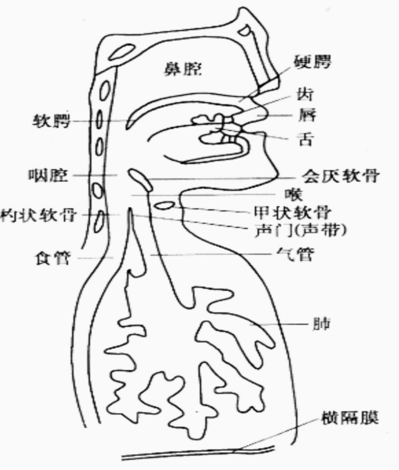
\includegraphics[width=0.6\textwidth]{human_speech_arch.png}
    \caption{人类发生机理 \label{fig:human_speech_arch}}
  \end{figure}

\subsection{语音合成的历史}
  
  语音合成系统分为两部分,分别称为前端和后端,如下图所示。

  \begin{figure}[htbp]
    \centering
    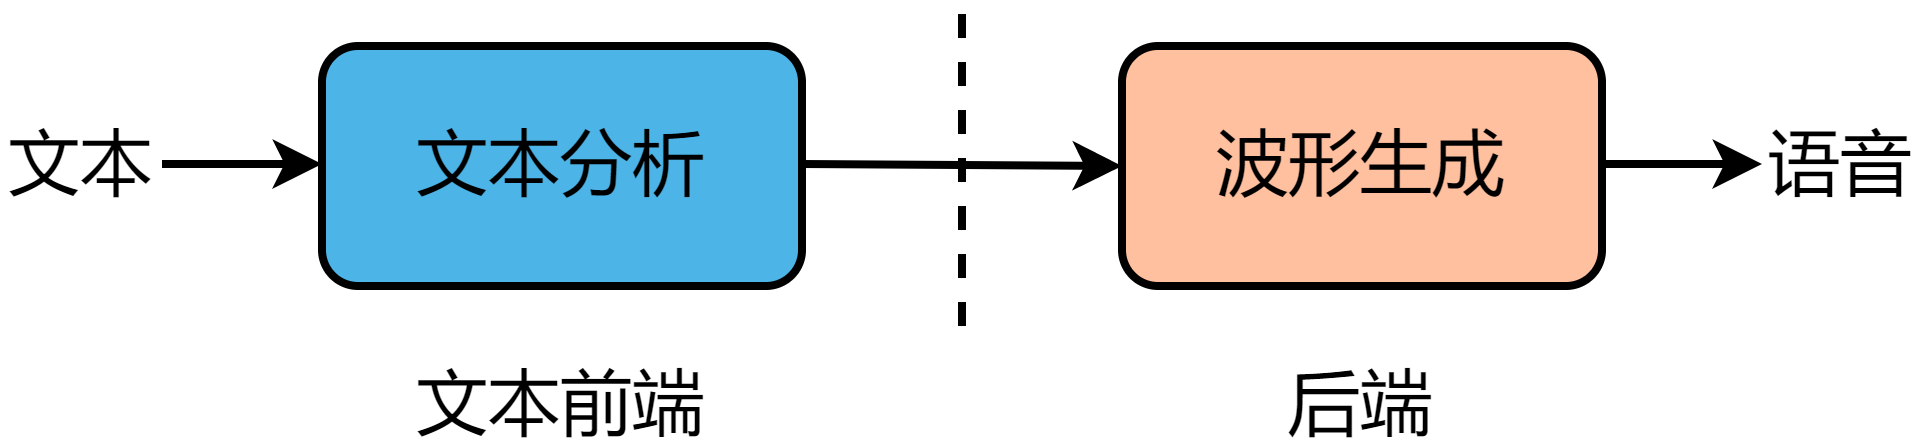
\includegraphics[width=0.6\textwidth]{text_to_speech_arch.png}
    \caption{语音合成系统框图 \label{fig:text_to_speech_arch}}
  \end{figure}

  前端主要负责在语言层、语法层、语义层对输入文本进行文本分析;后端主要是从信号处理、模式识别、机器学习等角度,在语音层面上进行韵律特征建模,声学特征建模,然后进行声学预测或者在音库中进行单元挑选,最终经过合成器或者波形拼接等方法合成语音。

  \begin{figure}[htbp]
    \centering
    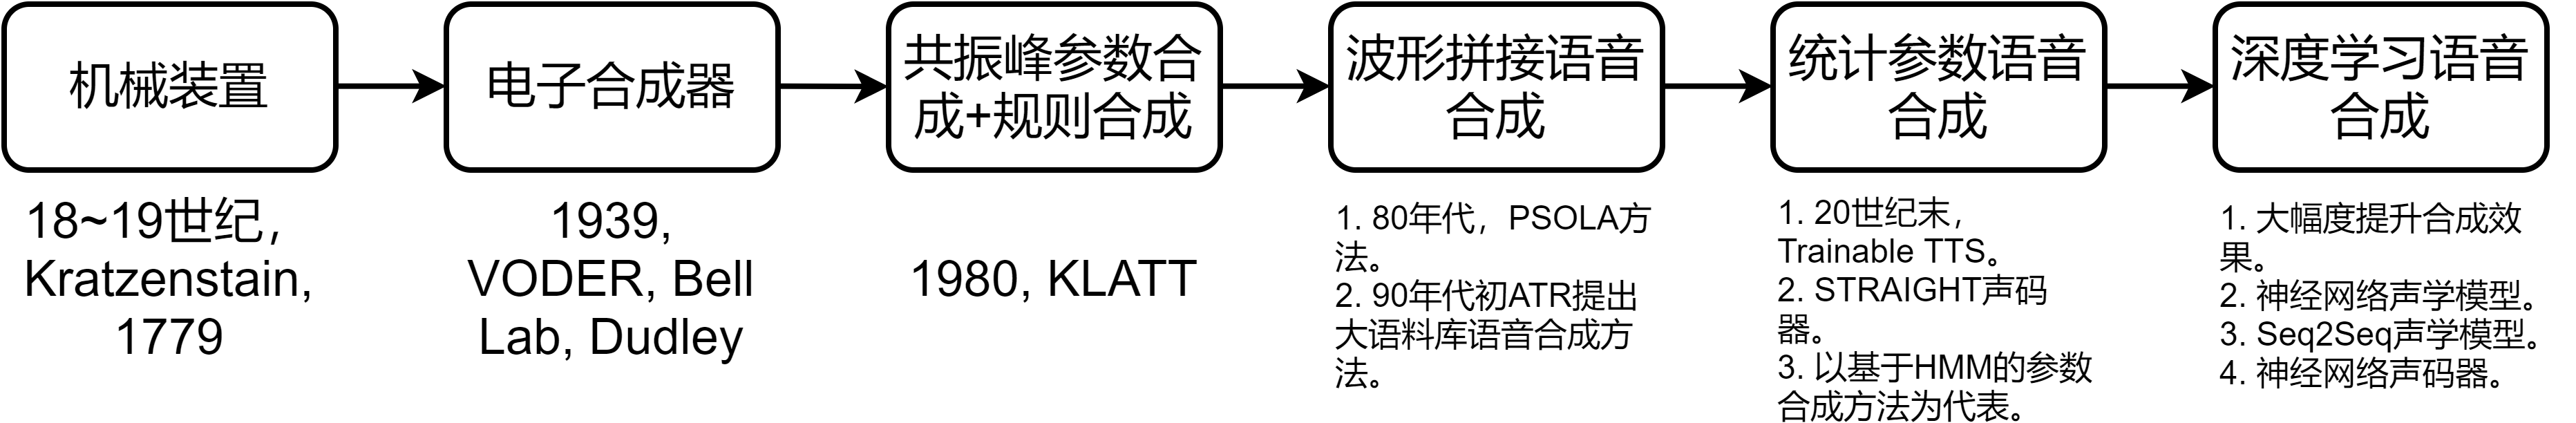
\includegraphics[width=0.9\textwidth]{text_to_speech_history.png}
    \caption{语音合成发展历史 \label{fig:text_to_speech_history}}
  \end{figure}

  根据语音合成研究的历史,如图\ref{fig:text_to_speech_history}所示,语音合成研究方法可以分为:机械式语音合成器、电子式语音合成器、共振峰参数合成器、基于波形拼接的语音合成、统计参数语音合成、以及神经网络语音合成。

  语音合成的早期工作主要是通过源-滤波器模型对语音产生的过程进行模拟。最开始的机械式语音合成器,使用风箱模拟人的肺部运动,产生激励空气流,采用振动弹簧片和皮革模拟声道系统,通过手动协调各部分运动,能够合成出五个长元音。机械式的语音合成器难以实用,随着时代的发展,贝尔实验室提出了电子式的语音合成器。不再模拟具体的生理器官,电子式语音合成器通过脉冲发射器和噪声发射器来分别产生模拟浊音和清音的激励系统,通过操作人员手动控制多个带通滤波器来模拟声道系统,最后通过放大器输出语音信号。由于电子式语音合成器使用有限个带通滤波器模拟声道系统,对自然语音的频谱特征的刻画精度有限。为了更好地刻画声道系统,共振峰参数合成器被提出。共振峰参数合成器将声道系统看成一个谐振腔,利用共振峰频率和宽度等声道的谐振特性,构建声道滤波器,以更好地刻画语音的声道特性。然而由于共振峰参数合成器结构复杂,需要大量人工分析调整参数,难以实用。

  早期的语音合成方法由于模型简单,系统复杂等原因,难以在实际场景应用。随着计算机技术的发展,基于波形拼接的语音合成被提出。基于波形拼接的语音合成的基本原理是首先构建一个音库,在合成阶段,通过对合成文本的分析,按照一定的准则,从音库中挑选出与待合成语音相似的声学单元,对这些声学单元进行少量调整,拼接得到合成的语音。早期的波形拼接系统受限于音库大小、挑选算法、拼接调整的限制,合成语音质量较低。 1990 年,基于同步叠加的时域波形修改算法被提出,解决了声学单元拼接处的局部不连续问题。更进一步,基于大语料库的波形拼接语音合成方法被提出,采用更精细的挑选策略,将语音音库极大地拓展,大幅提升了合成语音的自然度。由于直接使用发音人的原始语音,基于波形拼接的语音合成方法合成语音的音质接近自然语音,被广泛应用。但其缺点也较为明显,包括音库制作时间长、需要保存整个音库、拓展性差、合成语音自然度受音库和挑选算法影响,鲁棒性不高等。

  随着统计建模理论的完善,以及对语音信号理解的深入,基于统计参数的语音合成方法被提出。其基本原理是使用统计模型,对语音的参数化表征进行建模。在合成阶段,给定待合成文本,使用统计模型预测出对应的声学参数,经过声码器合成语音波形。统计参数语音合成方法是目前的主流语音合成方法之一。统计参数音合成方法的优点很多,包括只需要较少的人工干预,能够快速地自动构建系统,同时具有较强的灵活性,能够适应不同发音人,不同发音风格,多语种的语音合成,具有较强的鲁棒性等。由于语音参数化表示以及统计建模的平均效应,统计参数语音合成方法生成的语音自然度相比自然语音通常会有一定的差距。基于隐马尔科夫的统计参数语音合成方法是发展最为完善一种。基于 HMM 的统计参数语音合成系统能够同时对语音的基频、频谱和时长进行建模,生成出连续流畅且可懂度高的语音,被广泛应用,但其合成音质较差。

\subsection{当代语音合成框架}

和统计参数语音合成系统类似,深度学习语音合成系统也可大致分为两个部分:文本前端和声学后端。文本前端的主要作用是文本预处理,如:为文本添加韵律信息,并将文本词面转化为语言学特征序列(Linguistic Feature Sequence);声学后端又可以分为声学特征生成网络和声码器,其中声学特征生成网络根据文本前端输出的信息产生声学特征,如:将语言学特征序列映射到梅尔频谱或线性谱;声码器利用频谱等声学特征,生成语音样本点并重建时域波形,如:将梅尔频谱恢复为对应的语音。近年来,也出现了完全端到端的语音合成系统,将声学特征生成网络和声码器和合并起来,声学后端成为一个整体,直接将语言学特征序列,甚至文本词面端到端转换为语音波形。

\begin{enumerate}
  \item 文本前端
  
  文本前端的作用是从文本中提取发音和语言学信息,其任务至少包括以下四点。
  
  \begin{enumerate}
    \item 文本正则化
    
    在语音合成中,用于合成的文本存在特殊符号、阿拉伯数字等,需要把符号转换为文本。如“1.5元”需要转换成“一点五元”,方便后续的语言学分析。

    \item 韵律预测
    
    该模块的主要作用是添加句子中韵律停顿或起伏。如“在抗击新型冠状病毒的战役中,党和人民群众经受了一次次的考验”,如果停顿信息不准确就会出现:“在/抗击/新型冠状病毒/的/战役中,党/和/人民群众/经受了/一次/次/的/考验”。“一次次”的地方存在一个错误停顿,这将会导致合成语音不自然,如果严重些甚至会影响语义信息的传达。

    \item 字形转音素
    
    将文字转化为发音信息。比如“中国”是汉字表示,需要先将其转化为拼音“zhong1 guo2”,以帮助后续的声学模型更加准确地获知每个汉字的发音情况。

    \item 多音字和变调
    
    许多语言中都有多音字的现象,比如“模型”和“模样”,这里“模”字的发音就存在差异。另外,汉字中又存在变调现象,如“一个”和“看一看”中的“一”发音音调不同。所以在输入一个句子的时候,文本前端就需要准确判断出文字中的特殊发音情况,否则可能会导致后续的声学模型合成错误的声学特征,进而生成不正确的语音。
  \end{enumerate}

  \item 声学特征生成网络
  
  声学特征生成网络根据文本前端的发音信息,产生声学特征,如梅尔频谱或线性谱。近年来,基于深度学习的生成网络甚至可以去除文本前端,直接由英文等文本生成对应的频谱。但是一般来说,因为中文字形和读音关联寥寥,因此中文语音合成系统大多无法抛弃文本前端,换言之,直接将中文文本输入到声学特征生成网络中是不可行的。基于深度学习的声学特征生成网络发展迅速,比较有代表性的模型有Tacotron系列,FastSpeech系列等。近年来,也涌现出类似于VITS的语音合成模型,将声学特征生成网络和声码器融合在一起,直接将文本映射为语音波形。

  \item 声码器
  
  通过声学特征产生语音波形的系统被称作声码器,声码器是决定语音质量的一个重要因素。一般而言,声码器可以分为以下4类:纯信号处理,如Griffin-Lim、STRAIGHT和WORLD;自回归深度网络模型,如WaveNet和WaveRNN;非自回归模型,如Parallel WaveNet、ClariNet和WaveGlow;基于生成对抗网络(Generative Adversarial Network,GAN)的模型,如MelGAN、Parallel WaveGAN和HiFiGAN。

\end{enumerate}


\section{Awesome List}
\begin{enumerate}
  \item https://github.com/wenet-e2e/speech-synthesis-paper
  \item https://github.com/ddlBoJack/Speech-Resources
  \item https://github.com/sindresorhus/awesome
\end{enumerate}

\section{参考书籍}
\begin{enumerate}
  \item \href{https://nndl.github.io/}{神经网络与深度学习}
  \item Tan X, Qin T, Soong F, et al. A survey on neural speech synthesis[J]. arXiv preprint arXiv:2106.15561, 2021.
\end{enumerate}

\section{语音相关的会议、期刊、比赛和公司}
\subsection{会议}
\begin{enumerate}
  \item INTERSPEECH(Conference of the International Speech Communication Association)
  \item ICASSP(IEEE International Conference on Acoustics, Speech and Signal Processing)
  \item ASRU(IEEE Automatic Speech Recognition and Understanding Workshop)
  \item ISCSLP(International Symposium on Chinese Spoken Language Processing)
  \item ACL(Association of Computational Linguistics)
\end{enumerate}

\subsection{期刊}
\begin{enumerate}
  \item Computer Speech and Language
\end{enumerate}

\subsection{最新论文}
\begin{enumerate}
  \item \href{http://yqli.tech/page/tts_paper.html}{低调奋进TTS最新论文集}
  \item https://arxiv.org/list/eess.AS/recent
  \item https://arxiv.org/list/cs.SD/recent
  \item https://arxiv.org/list/cs.CL/recent
  \item https://arxiv.org/list/cs.MM/recent
\end{enumerate}

\subsection{比赛}
\begin{enumerate}
  \item Blizzard Challenge
  \item CHiME: Computational Hearing in Multisource Environment
  \item NIST
\end{enumerate}

\subsection{公司}
\begin{enumerate}
  \item \href{https://azure.microsoft.com/en-us/services/cognitive-services/text-to-speech/#features}{微软}
  \item \href{https://cloud.google.com/text-to-speech/docs/voices?hl=zh-cn}{谷歌云}
  \item \href{https://www.aicloud.com/dev/ability/index.html?key=tts#ability-experience}{捷通华声}
  \item \href{https://www.nuance.com/omni-channel-customer-engagement/voice-and-ivr/text-to-speech.html#!}{Nuance}
  \item \href{https://aws.amazon.com/cn/polly/}{Amazon polly}
  \item \href{https://fanyi.baidu.com/}{百度(翻译)}
  \item \href{https://ai.sogou.com/product/audio_composition/}{搜狗开发平台}
  \item \href{https://fanyi.sogou.com/}{搜狗(翻译)}
  \item \href{https://ai.youdao.com/product-tts.s}{有道开放平台}
  \item \href{http://fanyi.youdao.com}{有道(翻译)}
  \item \href{https://cn.bing.com/translator}{微软(翻译)}
  \item \href{https://translate.google.cn/}{Google翻译}
\end{enumerate}

\subsection{微信公众号}

\subsection{CCF语音对话与听觉专业组}
\begin{enumerate}
  \item https://history.ccf.org.cn/tfsdap/index.html
\end{enumerate}

\section{数据集}
\subsection{中文数据集}
\begin{enumerate}
  \item \href{https://www.data-baker.com/open_source.html}{标贝中文标准女声音库}: 中文单说话人语音合成数据集,质量高。
  \item \href{https://www.openslr.org/18/}{THCHS-30}: 中文多说话人数据集,原为语音识别练手级别的数据集,也可用于多说话人中文语音合成。
  \item \href{https://www.openslr.org/38/}{Free ST Chinese Mandarin Corpus}: 855个说话人,每个说话人120句话,有对应人工核对的文本,共102600句话。
  \item \href{https://github.com/KuangDD/zhvoice}{zhvoice}: zhvoice语料由8个开源数据集,经过降噪和去除静音处理而成,说话人约3200个,音频约900小时,文本约113万条,共有约1300万字。
  \item \href{https://arxiv.org/abs/2010.09275}{滴滴800+小时DiDiSpeech语音数据集}: DiDi开源数据集,800小时,48kHz,6000说话人,存在对应文本,背景噪音干净,适用于音色转换、多说话人语音合成和语音识别,参见:https://zhuanlan.zhihu.com/p/268425880。
  \item \href{https://github.com/khiajohnson/SpiCE-Corpus}{SpiCE-Corpus}: SpiCE是粤语和英语会话双语语料库。
\end{enumerate}

\subsection{英文数据集}
\begin{enumerate}
  \item \href{https://keithito.com/LJ-Speech-Dataset/}{LJSpeech}: 英文单说话人语音合成数据集,质量较高。
  \item \href{https://datashare.is.ed.ac.uk/handle/10283/2651}{VCTK}: 英文多说话人语音数据集,109个说话人,每人400句话,采样率48kHz,位深16bits。
  \item \href{https://catalog.ldc.upenn.edu/LDC93S1}{TIMIT}: 630个说话人,8个美式英语口音,每人10句话,采样率16kHz,位深16bits。\href{http://academictorrents.com/details/34e2b78745138186976cbc27939b1b34d18bd5b3}{这里是具体下载地址},下载方法:首先下载种子,然后执行:
  \begin{lstlisting}
    ctorrent *.torrent
  \end{lstlisting}

  \item \href{http://festvox.org/cmu_arctic/packed/}{CMU ARCTIC}: 共18个说话人。语音质量较高,可以用于英文多说话人的训练。

\end{enumerate}

\subsection{情感数据集}
\begin{enumerate}
  \item \href{https://github.com/HLTSingapore/Emotional-Speech-Data}{ESD}: 用于语音合成和语音转换的情感数据集。
  \item \href{https://github.com/Emotional-Text-to-Speech/dl-for-emo-tts}{情感数据和实验总结}: 实际是情感语音合成的实验总结,包含了一些情感数据集的总结。
\end{enumerate}

\subsection{其它数据集}
\begin{enumerate}
  \item \href{https://wenet.org.cn/opencpop}{Opencpop}: 高质量歌唱合成数据集。
  \item \href{https://ai.100tal.com/dataset}{好未来开源数据集}: 目前主要开源了3个大的语音数据集,分别是语音识别数据集,语音情感数据集和中英文混合语音数据集,都是多说话人教师授课音频。
  \item \href{http://www.aishelltech.com/aishell_2}{AISHELL-2}: 希尔贝壳开源了不少中文语音数据集,AISHELL-2是最近开源的一个1000小时的语音数据库,禁止商用。官网上还有其它领域,比如用于语音识别的4个开源数据集。
  \item \href{https://github.com/Kyubyong/css10}{CSS10}: 十个语种的单说话人语音数据的集合。
  \item \href{https://www.openslr.org/resources.php}{OpenSLR}: OpenSLR是一个专门托管语音和语言资源的网站,例如语音识别训练语料库和与语音识别相关的软件。迄今为止,已经有100+语音相关的语料。
  \item \href{https://github.com/jim-schwoebel/voice_datasets}{voice datasets}: Github上较为全面的开源语音和音乐数据集列表,包括语音合成、语音识别、情感语音数据集、语音分离、歌唱等语料,找不到语料可以到这里看看。
  \item \href{https://github.com/JRMeyer/open-speech-corpora}{Open Speech Corpora}: 开放式语音数据库列表,特点是包含多个语种的语料。
  \item \href{https://www.emime.org/participate.html}{EMIME}: 包含一些TTS和ASR模型,以及一个中文/英语,法语/英语,德语/英语双语数据集。
  \item \href{https://github.com/celebrity-audio-collection/videoprocess}{Celebrity Audio Extraction}: 中国名人数据集,包含中国名人语音和图像数据。
\end{enumerate}

\subsection{开源工具}
\begin{enumerate}
  \item \href{https://github.com/waywardgeek/sonic}{sonic}: 语音升降速工具。
  \item \href{https://github.com/MontrealCorpusTools/Montreal-Forced-Aligner/releases/download/v1.0.1/montreal-forced-aligner_linux.tar.gz}{MFA}: 从语音识别工具Kaldi中提取出来的音素-音频对齐工具,可以利用MFA获取每一个音素的时长,供预标注或时长模型使用。
  \item \href{https://github.com/jaekookang/p2fa_py3}{宾西法尼亚大学强制对齐标注软件(P2FA)}:\href{https://blog.csdn.net/jojozhangju/article/details/51951622}{这里}有相关的介绍,对于噪音数据鲁棒性差。
  \item \href{https://github.com/bootphon/ABXpy}{ABXpy}: 语音等测评ABX测试网页。
  \item \href{https://github.com/bigpon/SpeechSubjectiveTest}{SpeechSubjectiveTest}: 主观测评工具,包括用于语音合成和转换的MOS、PK(倾向性测听)、说话人相似度测试和ABX测试。
  \item \href{https://github.com/matpool/matools}{Matools}: 机器学习环境配置工具库
  \item \href{https://github.com/Alinshans/MyTinySTL}{MyTinySTL}: 基于C++11的迷你STL。
  \item \href{https://github.com/applenob/Cpp_Primer_Practice}{CppPrimerPractice}: 《C++ Primer 中文版(第 5 版)》学习仓库。
  \item \href{https://github.com/521xueweihan/git-tips}{git-tips}: Git的奇技淫巧。
\end{enumerate}

\subsection{开源项目}
\begin{enumerate}
  \item \href{https://github.com/coqui-ai/TTS}{coqui-ai TTS}: 采用最新研究成果构建的语音合成后端工具集。
  \item \href{https://github.com/espnet/espnet}{ESPNet}: 语音合成和识别工具集,主要集成声学模型、声码器等后端模型。
  \item \href{https://github.com/pytorch/fairseq}{fairseq}: 序列到序列建模工具,包含语音识别、合成、机器翻译等模型。
  \item \href{https://github.com/espeak-ng/espeak-ng}{eSpeak NG Text-to-Speech}: 共振峰生成的语音合成模型,集成超过100个语种和口音的语音合成系统,特别地,可借鉴该项目中的多语种文本前端。
  \item \href{https://github.com/dmort27/epitran}{Epitran}: 将文本转换为IPA的工具,支持众多语种。
  \item \href{https://github.com/Rayhane-mamah/Tacotron-2}{Tacotron-2}: Tensorflow版本的Tacotron-2.
  \item \href{https://github.com/as-ideas/TransformerTTS}{Transformer TTS}: TensorFlow 2实现的FastSpeech系列语音合成。
  \item \href{https://github.com/syoyo/tacotron-tts-cpp}{Text-to-speech in (partially) C++ using Tacotron model + Tensorflow}: 采用TensorFlow C++ API运行Tacotron模型。
  \item \href{https://github.com/microsoft/muzic}{muzic}: 微软AI音乐的开源项目,包括乐曲理解、音乐生成等多种工作。
  \item \href{https://github.com/CSTR-Edinburgh/merlin}{merlin}: CSTR开发的统计参数语音合成工具包,需要与文本前端(比如Festival)和声码器(比如STRAIGHT或WORLD)搭配使用。
\end{enumerate}

\section{语音合成评价指标}
对合成语音的质量评价,主要可以分为主观和客观评价。主观评价是通过人类对语音进行打分,比如平均意见得分(Mean Opinion Score,MOS)、众包平均意见得分(CrowdMOS,CMOS)和ABX测试。客观评价是通过计算机自动给出语音音质的评估,在语音合成领域研究的比较少,论文中常常通过展示频谱细节,计算梅尔倒谱失真(Mel Cepstral Distortion,MCD)等方法作为客观评价。客观评价还可以分为有参考和无参考质量评估,这两者的主要判别依据在于该方法是否需要标准信号。有参考评估方法除了待评测信号,还需要一个音质优异的,可以认为没有损伤的参考信号。常见的有参考质量评估主要有ITU-T P.861 (MNB)、ITU-T P.862 (PESQ)、ITU-T P.863 (POLQA)、STOI和BSSEval。无参考评估方法则不需要参考信号,直接根据待评估信号,给出质量评分,无参考评估方法还可以分为基于信号、基于参数以及基于深度学习的质量评估方法。常见的基于信号的无参考质量评估包括ITU-T P.563和ANIQUE+,基于参数的方法有ITU-T G.107(E-Model)。近年来,深度学习也逐步应用到无参考质量评估中,如:AutoMOS、QualityNet、NISQA和MOSNet。

主观评价中的MOS评测是一种较为宽泛的说法,由于给出评测分数的主体是人类,因此可以灵活测试语音的不同方面。比如在语音合成领域,主要有自然度MOS(MOS of Naturalness)和相似度MOS(MOS of Similarity)。但是人类给出的评分结果受到的干扰因素较多,谷歌对合成语音的主观评估方法进行了比较,在评估较长语音中的单个句子时,音频样本的呈现形式会显著影响参与人员给出的结果。比如仅提供单个句子而不提供上下文,与相同句子给出语境相比,被测人员给出的评分差异显著。国际电信联盟(International Telecommunication Union,ITU)将MOS评测规范化为ITU-T P.800,其中绝对等级评分(Absolute Category Rating,ACR)应用最为广泛,同时也是本文中采用的语音质量评估标准,ACR的详细评估标准如下表所示。

\begin{table}[htbp]
  \centering
  \caption{主观意见得分的评估标准}
    \begin{tabular}{llll}
    \toprule
    音频级别 & 平均意见得分 & 评价标准 \\
    \midrule
    优 & 5.0 & 很好,听得清楚;延迟小,交流流畅 \\
    良 & 4.0 & 稍差,听得清楚;延迟小,交流欠流畅,有点杂音 \\
    中 & 3.0 & 还可以,听不太清;有一定延迟,可以交流 \\
    差 & 2.0 & 勉强,听不太清;延迟较大,交流需要重复多遍 \\
    劣 & 1.0 & 极差,听不懂;延迟大,交流不通畅 \\
    \bottomrule
    \end{tabular}%
\end{table}%

在使用ACR方法对语音质量进行评价时,参与评测的人员(简称被试)对语音整体质量进行打分,分值范围为1~5分,分数越大表示语音质量越好。MOS大于4时,可以认为该音质受到大部分被试的认可,音质较好;若MOS低于3,则该语音有比较大的缺陷,大部分被试并不满意该音质。

\section{平均意见得分的测评要求与方法}
语音合成的最终目标是,合成语音应尽可能接近真实发音,以至于人类无法区分合成和真实语音。因此让人类对合成语音进行评价打分是最为直观的评价方法,评分经处理之后即可获得平均意见得分。平均意见得分是语音合成系统最重要的性能指标之一,能够直接反映合成语音的自然度、清晰度以及可懂度。
\subsection{实验要求}
获取多样化且数量足够大的音频样本,以确保结果在统计上的显著,测评在具有特定声学特性的设备上进行,控制每个被试遵循同样的评估标准,并且确保每个被试的实验环境保持一致。
\subsection{实验方法}
为了达到实验要求,可以通过两种方法获得足够精确的测评结果。第一种是实验室方式,该方式让被试在实验室环境中进行测评,在试听过程中环境噪音必须低于35dB,测试语音数量至少保持30个以上,且覆盖该语种所有音素和音素组合,参与评测的被试应尽可能熟练掌握待测合成语音的语种,最好以合成语音的语种为母语。该方法的优点是测试要素容易控制,能够稳定保证实验环境达到测评要求;缺点则主要是需要被试在固定场所完成试听,人力成本高。第二种是众包,也就是将任务发布到网络上,让具有条件的被试在任何地方进行测评。该方法主要优点是易于获得较为有效的评估结果;而缺点则体现在无法确保试听条件。
\subsection{实验步骤}
\begin{enumerate}
  \item 收集合成语音和录制的真实语音;
  \item 确保文本和语音一一对应,去除发音明显错误的音频样本;
  \item 生成问卷,将合成语音和真实语音交叉打乱,确保打乱的顺序没有规律,合成语音和真实语音不可让被试提前探知到;
  \item 开始任务前,被试试听示例语音,并告知其对应的大致得分;
  \item 被试开始对给定音频打分,前三条语音可以作为被试进入平稳打分状态的铺垫,不计入最终结果;
  \item 回收问卷,舍弃有明显偏差的评价数据,统计最终得分。
\end{enumerate}

\subsection{实验设计}
\begin{enumerate}
  \item 准备测试语音数据。(1)从各领域和语音合成系统实际应用场景中,摘选常规文本作为测试语料,选取的语句一般尽可能排除生僻字;(2)用于测试的句子一般是未出现在训练集中的;(3)	被试必须使用耳机试听语音,以便于判断更为细微的差别;(4)为了避免被试的疲惫,待测评系统和语料数量不可太多,需要控制测评时间;(5)一个句子需要由多个被试打分。
  \item 设置实验参数。在准备测试语音时,需要提前设置好训练语料、待测系统、参与测试的句子数量、每个句子被试听的次数等。以中文语音合成系统的语音评估为例,测评设置如下表所示。
  \begin{table}[htbp]
    \centering
    \caption{语音测评设置}
      \begin{tabular}{llll}
      \toprule
      训练集 & 待测系统 & 句子数量 & 每个句子被测次数 \\
      \midrule
      内部数据集 & 真实语音 & 40 & 12 \\
      内部数据集 & Tacotron-2 & 40 & 12 \\
      内部数据集 & FastSpeech-2 & 40 & 12 \\
      \bottomrule
      \end{tabular}%
  \end{table}%

  \item 准备HTML文档等展示材料,向被试介绍该测试。该HTML文档至少包括:(1)测试注意事项,如被试应该使用何种设备,在何种环境下试听,试听时应该排除的干扰因素等;(2)测试任务,向被试介绍本次试听的测试目标,应关注的侧重点,如:可懂度、相似度、清晰度等方面;(3)参考音频,可以放置一些示例音频,如MOS=5的优质语音,MOS=1的低劣音频,以便被试更好地对音频打分;(4)	测试音频,根据不同任务,放置合理的测试音频,真实和合成音频应提前打乱,并且不可告知被试打乱的顺序。
  
\end{enumerate}

\subsection{实验数据处理}
\begin{enumerate}
  \item 数据筛选。由于被试有可能没有受到监督,因此需要对收集到的评分进行事后检查,如删除使用扬声器试听的评分。另外,为了控制个体因素对整体结果的影响,减少偏离整体数据的异常值,需要计算每个人的评分与总体得分序列的相关性,相关性的度量使用相关系数来实现,如果相关系数r大于0.25,则保留;否则拒绝该被试的所有评分。相关系数r的计算方法如下:
  \begin{equation}
    r=\frac{\mathop{cov}(\mu_{1n},...,\mu_{Mn};\mu_1,...,\mu_M)}{\sqrt{\mathop{var}(\mu_{1n},...,\mu_{Mn})}\cdot \sqrt{\mathop{var}(\mu_1,...,\mu_M)}}
  \end{equation}
\end{enumerate}

其中, $M$ 为句子数量,$N$为被试数量, $\mu_{mn}$ 为被试 $n$ 对句子 $m$ 给出的评分,$1\leq m\leq M$ ,$1\leq n\leq N$, $\mu_m=1/N\sum_{n=1}^N\mu_{mn}$ 为句子 $m$ 的总体平均分, $\mathop{cov}$ 为协方差, $\mathop{var}$ 为方差。

\chapter{语音信号基础}

\section{参考资料}

\begin{enumerate}
  \item \href{http://labrosa.ee.columbia.edu/~dpwe/pubs/Ellis10-introspeech.pdf}{An Introduction to Signal Processing for Speech}
  \item \href{https://www.inf.ed.ac.uk/teaching/courses/asr/2020-21/asr02-signal.pdf}{爱丁堡大学课件}
  
\end{enumerate}

\section{基本概念}
声波通过空气传播,被麦克风接收,通过 \lstinline{采样}、 \lstinline{量化}、 \lstinline{编码}转换为离散的数字信号,即波形文件。

\begin{enumerate}
  \item 波形(waveform): 声音是由声源振动产生的波
  \item 音高(pitch): 与频率(frequency)有关,是频谱上的第一共振峰。音高(pitch)是稀疏离散化的基频(f0)。
  \item 响度: 与振幅(amplitude)有关。
  \item 音色: 由频谱上的谐波决定。音高、响度和音色被称作声音的三要素。
  \item 信道: 通信的通道Channel,是信号传输的媒介。
  \item 声道: 声音在录制和播放时,在不同空间位置采集或回放相互独立的音频信号,因此声道数也就是声音录制时的音源数量或回放时相应的扬声器数量。
  \item 采样率:单位时间内从连续信号中提取并组成离散信号的采样个数,音频常用单位kHz。
  \item 采样位数/采样深度:数字信号的二进制位数,与每次采样的可能值个数有关,音频常用单位bit。常见的音频格式: \lstinline{16kHz,16bit}中16kHz指的是采样率,16bit表示采样位深。
  \item 信噪比(SNR):和声压级类似,单位仍采用分贝,数值越高,表示声音越干净,噪音比例越小。
  \item 音素(phoneme):声音的最小单位,同一音素由不同人/环境阅读,可以形成不同的发音。
  \item 字素(grapheme):音素对应的文本。具体的区别参见:\href{https://www.youtube.com/watch?v=25r1fyoorko}{Phonemes, Graphemes, and Morphemes!}
  \item phone: 某个音素的具体发音。
  \item 过零率
  \item 短时能量
  \item LPC。线性预测系数。LPC的基本思想是,当前时刻的信号可以用若干历史时刻信号的线性组合来估计,通过使实际语音的采样值和线性预测的采样值之间达到均方差最小,即可得到一组线性预测系数。求解LPC系数可以采用自相关法、协方差法、格型法等快速算法。
  \begin{note}
    语音信号的数字表示可以分为两类:\lstinline{波形表示}和\lstinline{参数表示},波形表示仅通过采样和量化保存模拟信号的波形;而参数表示将语音信号表示为某种语音产生模型的输出,是对数字化语音进行分析和处理之后得到的。
  \end{note}

  \begin{note}
    利用同态处理方法,对语音信号求离散傅里叶变换之后取对数,再求反变换就可以得到倒谱系数。其中,LPC倒谱(LPCCEP)是建立在LPC谱上的,而梅尔倒谱系数(Mel Frequency Cepstrum Coefficient,MFCC)则是基于梅尔频谱的。
  \end{note}

  \item LPCC。LPCC特征假定信号存在一种线性预测的结构,这对于周期特性的浊音描述比较准确,而对于辅音则相当于强加了一种错误的结构。MFCC相邻帧特征近乎独立,所以能够比较好地描述辅音,但忽略了信号可能的内在结构,如相邻帧之间的关联,经验表明MFCC更好用,并且经常会加入差分特征以减弱其独立性。
  \begin{note}
    线性预测倒谱系数(LPCC)是根据声管模型建立的特征参数,是对声道响应的特征表征。梅尔频谱倒谱系数(MFCC)是基于人类听觉机理提取出的特征参数,是对人耳听觉的特征表征。
  \end{note}
\end{enumerate}

对于一段1秒的波形,假设采样率16kHz,采样位深16bit,则包含样本点 $1\times 16000=16000$ 个,所占容量 $1\times 16000\times 16 /8=32000$ 字节(B)。

\section{音频格式}
\begin{enumerate}
  \item *.wav: 波形无损压缩格式,是语音合成中音频语料的常用格式,主要的三个参数:采样率,量化位数和通道数。一般来说,合成语音的采样率采用16kHz、22050Hz、24kHz,对于歌唱合成等高质量合成场景采样率可达到48kHz;量化位数采用16bit;通道数采用1.
  \item *.flac: Free Lossless Audio Codec,无损音频压缩编码。
  \item *.mp3: Moving Picture Experts Group Audio Player III,有损压缩。
  \item *.wma: Window Media Audio,有损压缩。
  \item *.avi: Audio Video Interleaved,avi文件将音频和视频包含在一个文件容器中,允许音视频同步播放。
\end{enumerate}

\section{发音学}

\section{数字信号处理}
\subsection{模数转换}

模拟信号到数字信号的转换(Analog to Digital Converter,ADC)称为模数转换。

奈奎斯特采样定理:要从抽样信号中无失真地恢复原信号,抽样频率应大于2倍信号最高频率。抽样频率小于2倍频谱最高频率时,信号的频谱有混叠。抽样频率大于2倍频谱最高频率时,信号的频谱无混叠。如果对语音模拟信号进行采样率为16000Hz的采样,得到的离散信号中包含的最大频率为8000Hz。

\subsection{傅里叶变换}

\subsection{频谱泄露}

音频处理中,经常需要利用傅里叶变换将时域信号转换到频域,而一次快速傅里叶变换(FFT)只能处理有限长的时域信号,但语音信号通常是长的,所以需要将原始语音截断成一帧一帧长度的数据块。这个过程叫\lstinline{信号截断},也叫\lstinline{分帧}。分完帧后再对每帧做FFT,得到对应的频域信号。FFT是离散傅里叶变换(DFT)的快速计算方式,而做DFT有一个先验条件:分帧得到的数据块必须是整数周期的信号,也即是每次截断得到的信号要求是周期主值序列。

但做分帧时,很难满足\lstinline{周期截断},因此就会导致\lstinline{频谱泄露}。要解决非周期截断导致的频谱泄露是比较困难的,可以通过\lstinline{加窗}尽可能减少频谱泄露带来的影响。窗类型可以分为汉宁窗、汉明窗、平顶窗等。虽然加窗能够减少频谱泄露,但加窗衰减了每帧信号的能量,特别是边界处的能量,这时加一个合成窗,且overlap-add,便可以补回能量。参见:\href{https://zhuanlan.zhihu.com/p/339692933}{频谱泄露和加窗}。

\subsection{频率分辨率}
频率分辨率是指将两个相邻谱峰分开的能力,在实际应用中是指分辨两个不同频率信号的最小间隔。


\chapter{语音特征提取}
原始信号是不定长的时序信号,不适合作为机器学习的输入。因此一般需要将原始波形转换为特定的特征向量表示,该过程称为语音特征提取。

\section{预处理}
包括预加重、分帧和加窗。

\subsection{预加重}
语音经过说话人的口唇辐射发出,受到唇端辐射抑制,高频能量明显降低。一般来说,当语音信号的频率提高两倍时,其功率谱的幅度下降约6dB,即语音信号的高频部分受到的抑制影响较大。在进行语音信号的分析和处理时,可采用预加重(pre-emphasis)的方法补偿语音信号高频部分的振幅,本质是施加低通滤波器。假设输入信号第 $n$ 个采样点为 $x[n]$ ,则预加重公式如下:

\begin{equation}
  x'[n]=x[n]-a\times x[n-1]
\end{equation}

其中, $a$ 是预加重系数,一般取 $a=0.97$。

\subsection{分帧}
语音信号是非平稳信号,考虑到发浊音时声带有规律振动,即基音频率在短时范围内时相对固定的,因此可以认为语音信号具有短时平稳特性,一般认为10ms~50ms的语音信号片段是一个准稳态过程。短时分析采用分帧方式,一般每帧帧长为20ms或50ms。假设语音采样率为16kHz,帧长为20ms,则一帧有 $16000\times 0.02=320$ 个样本点。

相邻两帧之间的基音有可能发生变化,如两个音节之间,或者声母向韵母过渡。为确保声学特征参数的平滑性,一般采用重叠取帧的方式,即相邻帧之间存在重叠部分。一般来说,帧长和帧移的比例为 $1:4$ 或 $1:5$ 。

\subsection{加窗}
分帧相当于对语音信号加矩形窗,矩形窗在时域上对信号进行截断,在边界处存在多个旁瓣,会发生频谱泄露。为了减少频谱泄露,通常对分帧之后的信号进行其它形式的加窗操作。常用的窗函数有:汉明(Hamming)窗、汉宁(Hanning)窗和布莱克曼(Blackman)窗等。

汉明窗的窗函数为:

\begin{equation}
  W_{ham}[n]=0.54-0.46\mathop{cos}(\frac{2\pi n}{N}-1)
\end{equation}

其中, $0\leq n\leq N-1$ ,$N$ 是窗的长度。

汉宁窗的窗函数为:

\begin{equation}
  W_{han}[n]=0.5[1-\mathop{cos}(\frac{2\pi n}{N}-1)]
\end{equation}

其中, $0\leq n\leq N-1$ , $N$ 是窗的长度。

\section{短时傅里叶变换}

人类听觉系统与频谱分析紧密相关,对语音信号进行频谱分析,是认识和处理语音信号的重要方法。声音从频率上可以分为纯音和复合音,纯音只包含一种频率的声音(基音),而没有倍音。复合音是除了基音之外,还包含多种倍音的声音。大部分语音都是复合音,涉及多个频率段,可以通过傅里叶变换进行频谱分析。

每个频率的信号可以用正弦波表示,采用正弦函数建模。基于欧拉公式,可以将正弦函数对应到统一的指数形式:

\begin{equation}
  e^{jwn}=\mathop{cos}(wn)+j\mathop{sin}(wn)
\end{equation}

正弦函数具有正交性,即任意两个不同频率的正弦波乘积,在两者的公共周期内积分等于零。正交性用复指数运算表示如下:

\begin{equation}
  \int_{-\infty}^{+\infty}e^{j\alpha t}e^{-j\beta t}dt=0,\quad if\ \alpha\neq \beta
\end{equation}

基于正弦函数的正交性,通过相关处理可以从语音信号分离出对应不同频率的正弦信号。对于离散采样的语音信号,可以采用离散傅里叶变换(DFT)。DFT的第 $k$ 个点计算如下:

\begin{equation}
  X[k]=\sum_{n=0}^{N-1} x[n]e^{-\frac{j2\pi kn}{K}},\quad k=0,1,...,K-1
\end{equation}

其中, $x[n]$ 是时域波形第 $n$ 个采样点值, $X[k]$ 是第 $k$ 个傅里叶频谱值, $N$ 是采样点序列的点数, $K$ 是频谱系数的点数,且 $K\geq N$ 。利用DFT获得的频谱值通常是复数形式,这是因为上式中,

\begin{equation}
  e^{-\frac{j2\pi kn}{K}}=\mathop{cos}(\frac{2\pi kn}{K})-j\mathop{sin}(\frac{2\pi kn}{K})
\end{equation}

则

\begin{equation}
  X[k]=X_{real}[k]-jX_{imag}[k]
\end{equation}

其中,

\begin{equation}
  X_{real}[k]=\sum_{n=0}^{N-1}x[n]\mathop{cos}(\frac{2\pi kn}{K})
\end{equation}

\begin{equation}
  X_{imag}[k]=\sum_{n=0}^{N-1}x[n]\mathop{sin}(\frac{2\pi kn}{K})
\end{equation}

$N$ 个采样点序列组成的时域信号经过DFT之后,对应 $K$ 个频率点。经DFT变换得到信号的频谱表示,其频谱幅值和相位随着频率变化而变化。

在语音信号处理中主要关注信号的频谱幅值,也称为振幅频谱/振幅谱:

\begin{equation}
  X_{magnitude}[k]=\sqrt{X_{real}[k]^2+X_{imag}[k]^2}
\end{equation}

能量频谱/能量谱是振幅频谱的平方:

\begin{equation}
  X_{power}[k]=X_{real}[k]^2+X_{imag}[k]^2
\end{equation}

各种声源发出的声音大多由许多不同强度、不同频率的声音组成复合音,在复合音中,不同频率成分与能量分布的关系称为声音的频谱,利用频谱图表示各频率成分与能量分布之间的关系,频谱图横轴是频率(Hz),纵轴是幅度(dB)。

通过对频域信号进行逆傅里叶变换(IDFT),可以恢复时域信号:

\begin{equation}
  x[n]=\frac{1}{K}\sum_{k=0}^{K-1}X[k]e^{\frac{j2\pi kn}{N}},\quad n=0,1,...,N-1
\end{equation}

离散傅里叶变换(DFT)的计算复杂度为 $O(N^2)$ ,可以采用快速傅里叶变换(FFT),简化计算复杂度,在 $O(N\mathop{log}_2 N)$ 的时间内计算出DFT。在实际应用中,对语音信号进行分帧加窗处理,将其分割成一帧帧的离散序列,可视为短时傅里叶变换(STFT):

\begin{equation}
  X[k,l]=\sum_{n=0}^{N-1} x_l[n]e^{-\frac{j2\pi nk}{K}}=\sum_{n=0}^{N-1} w[n]x[n+lL]e^{-\frac{j2\pi nk}{K}}
\end{equation}

其中, $K$ 是DFT后的频率点个数, $k$ 是频率索引, $0\leq k< K$ 。$X[k,l]$ 建立起索引为 $lL$ 的时域信号,与索引为 $k$ 的频域信号之间的关系。

\section{听觉特性}

\subsection{梅尔滤波}

人类对不同频率的语音有不同的感知能力:

\begin{enumerate}
  \item 1kHz以下,人耳感知与频率成线性关系。
  \item 1kHz以上,人耳感知与频率成对数关系。
\end{enumerate}

因此,人耳对低频信号比高频信号更为敏感。因此根据人耳的特性提出了一种mel刻度,即定义1个mel刻度相当于人对1kHz音频感知程度的千分之一,mel刻度表达的是,从线性频率到“感知频率”的转换关系:

\begin{equation}
  mel(f)=2595\mathop{lg}(1+\frac{f}{700})
\end{equation}

\begin{lstlisting}
  from matplotlib import pyplot as plt
  import numpy as np

  x = np.linspace(0, 5000, 50000)
  y = 2595*np.log10(1+x/700)
  x0 = 1000
  y0 = 2595*np.log10(1+x0/700)
  plt.plot(x, y)
  plt.scatter(x0, y0)
  plt.plot([x0, x0], [0, y0], 'k--')
  plt.plot([0, x0], [x0, y0], 'k--')
  plt.xlabel('f (Hz)')
  plt.ylabel('Mel(f)')
  plt.title('relationship between linear and mel scale')
  plt.xlim(0, x[-1])
  plt.ylim(0, y[-1])
  plt.savefig('mel_vs_f.png')
  plt.show()
\end{lstlisting}

\begin{figure}[htbp]
  \centering
  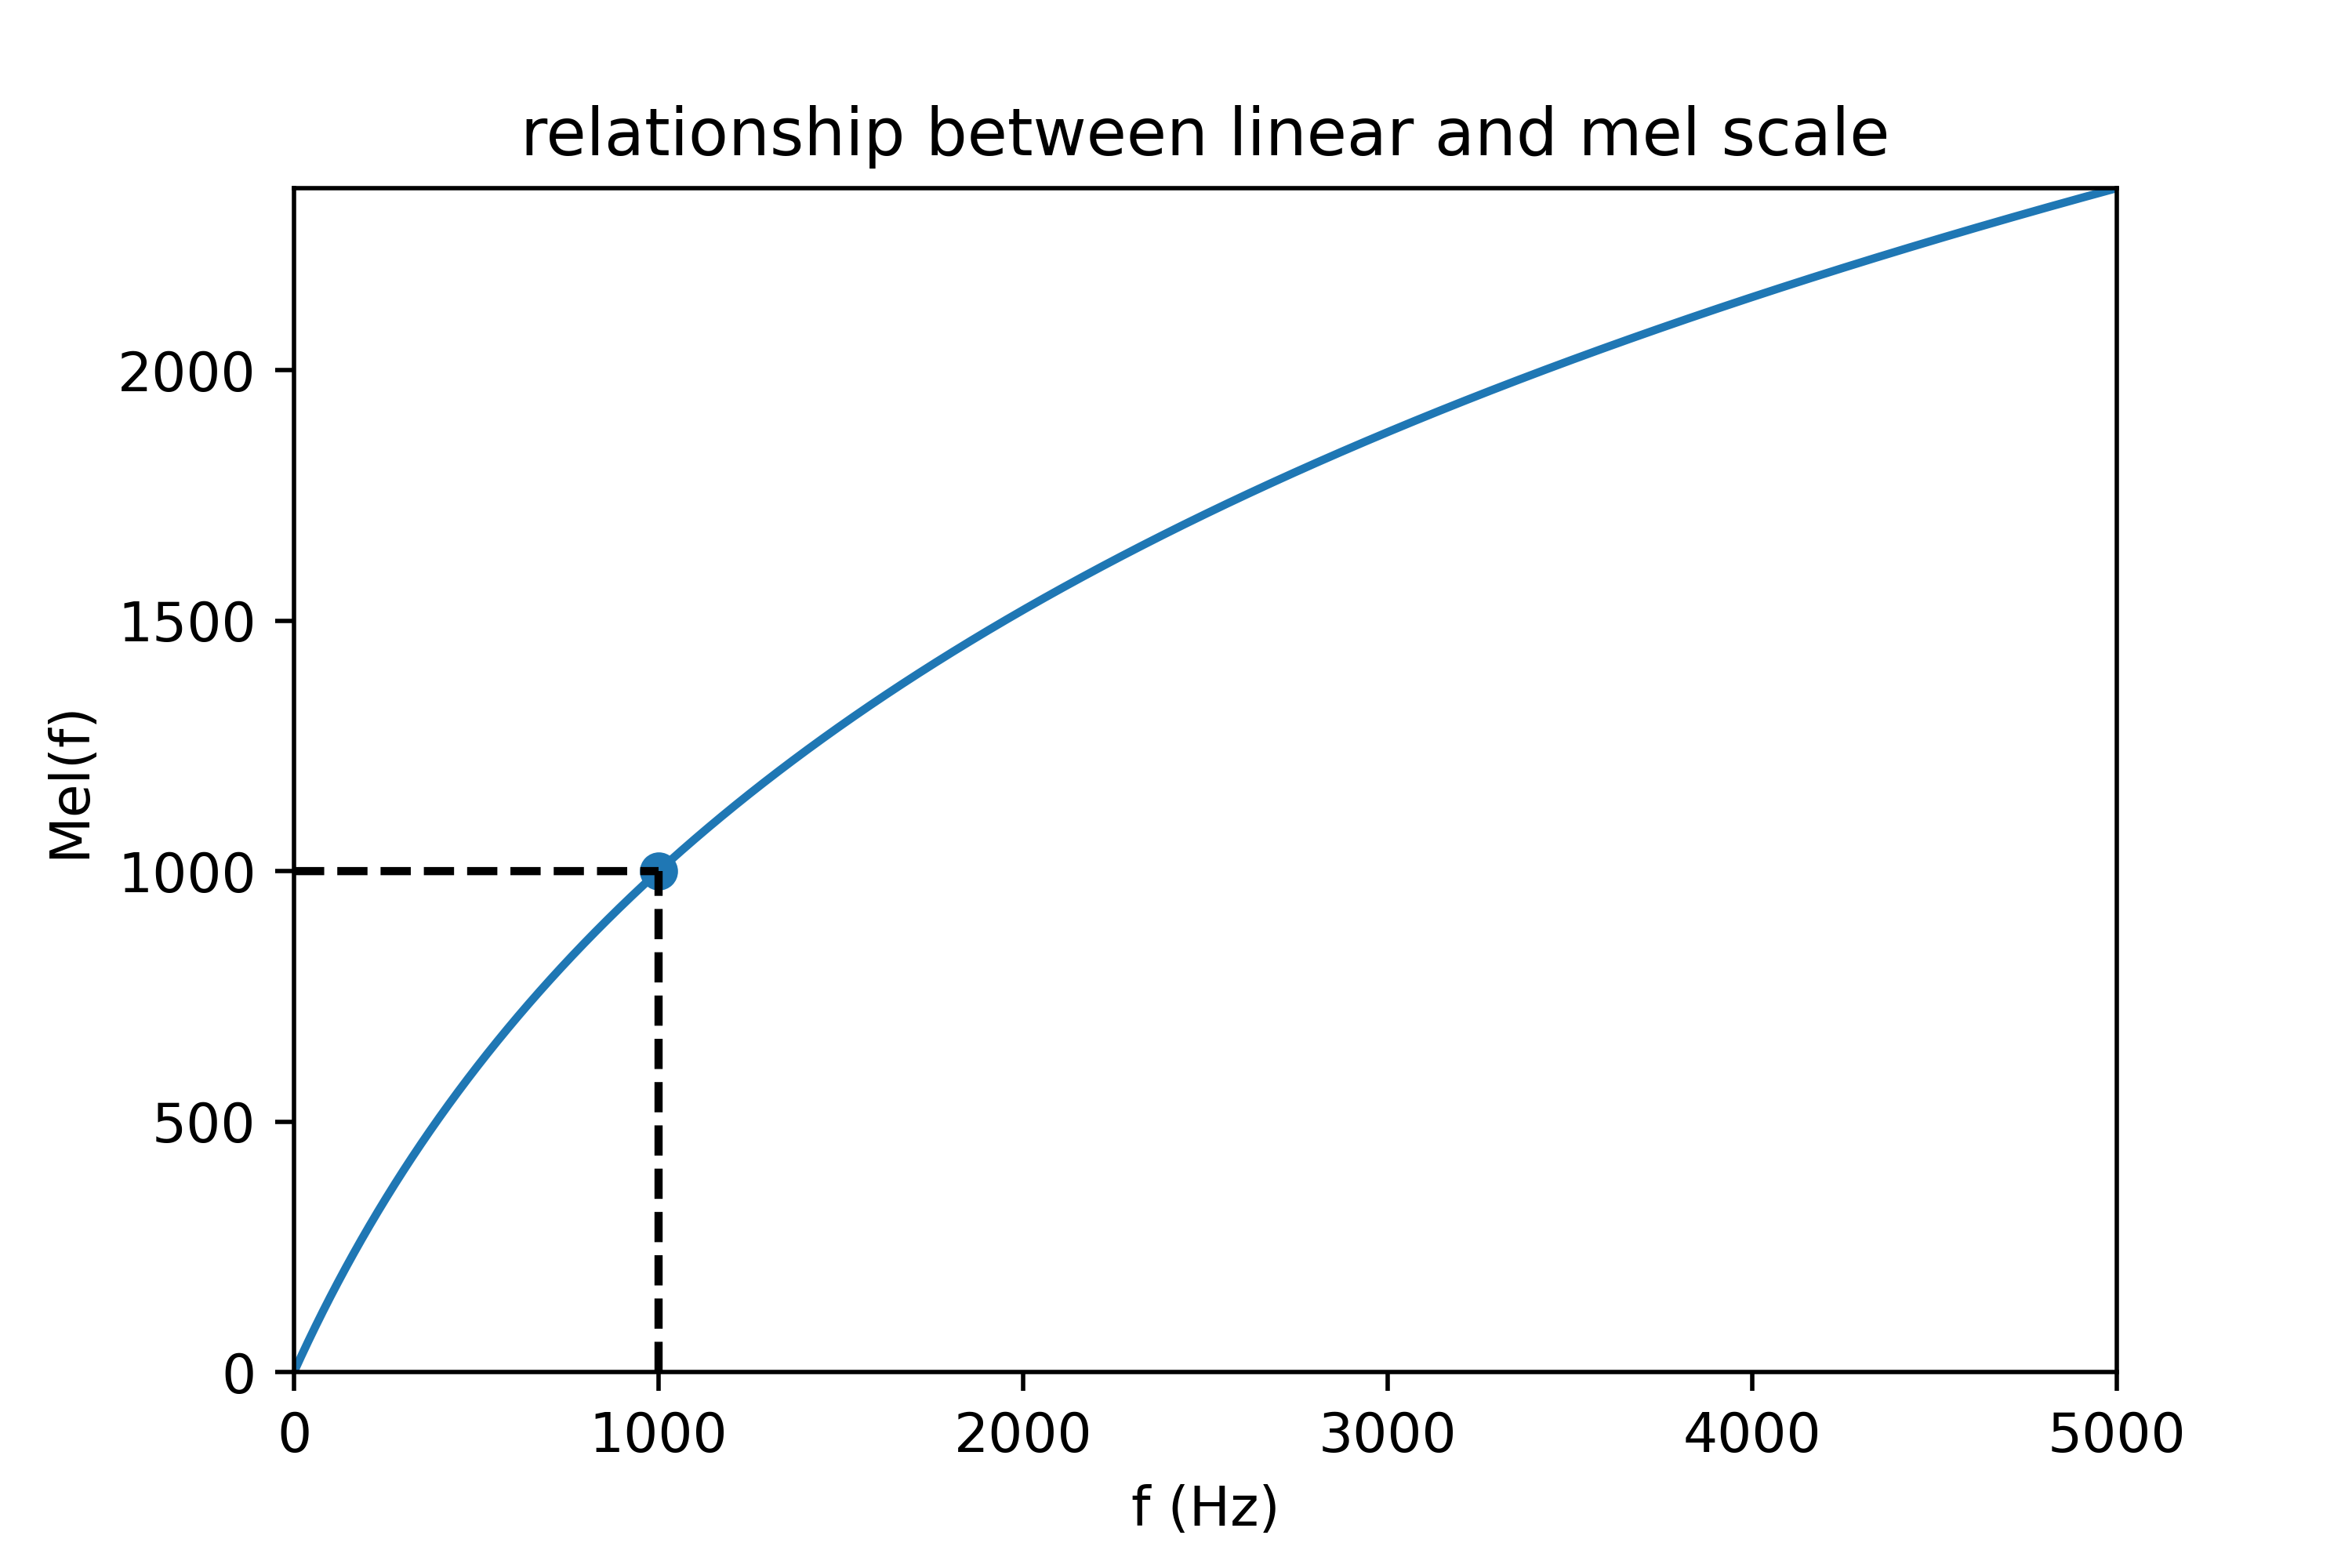
\includegraphics[width=0.6\textwidth]{mel_vs_f.png}
  \caption{mel刻度和频率之间的关系 \label{fig:mel_vs_f}}
\end{figure}

人们根据一系列心理声学实验得到了类似耳蜗作用的滤波器组,用于模拟人耳不同频段声音的感知能力,也就是多个三角滤波器组成的mel频率滤波器组。每个滤波器带宽不等,线性频率小于1000Hz的部分为线性间隔,而线性频率大于1000Hz的部分为对数间隔。同样地,将梅尔频率转换到线性频率的公式为:

\begin{equation}
  f_{mel}^{-1}=700\cdot (10^{\frac{f_{mel}}{2595}}-1)
\end{equation}

\subsection{Bark滤波}

声音的响度,反映人对不同频率成分声强/声音强弱的主观感受。响度与声强、频率的关系可以用\lstinline{等响度轮廓曲线}表示。

人耳对响度的感知有一个范围,当声音低于某个响度时,人耳是无法感知到的,这个响度值称为听觉阈值,或称听阈。在实际环境中,但一个较强信号(掩蔽音)存在时,听阈就不等于安静时的阈值,而是有所提高。这意味着,邻近频率的两个声音信号,弱响度的声音信号会被强响度的声音信号所掩蔽(Mask),这就是\lstinline{频域掩蔽}。

根据听觉频域分辨率和频域掩蔽的特点,定义能够引起听觉主观变化的频率带宽为一个\lstinline{临界频带}。一个临界频带的宽度被称为一个Bark,Bark频率 $Z(f)$ 和线性频率 $f$ 的对应关系定义如下:

\begin{equation}
  Z(f)=6\mathop{ln}(\frac{f}{600}+((\frac{f}{600})^2+1)^{\frac{1}{2}})
\end{equation}

其中,线性频率 $f$ 的单位为Hz,临界频带 $Z(f)$ 的单位为Bark。

\section{倒谱分析}

语音信号的产生模型包括发生源(Source)和滤波器(Filter)。人在发声时,肺部空气受到挤压形成气流,气流通过声门(声带)振动产生声门源激励 $e[n]$ 。对于浊音,激励 $e[n]$ 是以基音周期重复的单位冲激;对于清音, $e[n]$ 是平稳白噪声。该激励信号 $e[n]$ 经过咽喉、口腔形成声道的共振和调制,特别是舌头能够改变声道的容积,从而改变发音,形成不同频率的声音。气流、声门可以等效为一个激励源,声道等效为一个时变滤波器,语音信号 $x[n]$ 可以被看成激励信号 $e[n]$ 与时变滤波器的单位响应 $v[n]$ 的卷积:

\begin{equation}
  x[n]=e[n]*v[n]
\end{equation}

已知语音信号 $x[n]$ ,待求出上式中参与卷积的各个信号分量,也就是解卷积处理。除了线性预测方法外,还可以采用\lstinline{倒谱分析}实现解卷积处理。倒谱分析,又称为\lstinline{同态滤波},采用时频变换,得到对数功率谱,再进行逆变换,分析出倒谱域的倒谱系数。

同态滤波的处理过程如下:

\begin{enumerate}
  \item 傅里叶变换。将时域的卷积信号转换为频域的乘积信号:
  \begin{equation}
    {\rm DFT}(x[n])=X[z]=E[z]V[z]
  \end{equation}
  \item 对数运算。将乘积信号转换为加性信号:
  \begin{equation}
    {\rm log} X[z]={\rm log}E[z]+{\rm log}V[z]=\hat{E}[z]+\hat{V}[z]=\hat{X}[z]
  \end{equation}
  \item 傅里叶反变换。得到时域的语音信号\lstinline{倒谱}。
  \begin{equation}
    Z^{-1}(\hat{X}[z])=Z^{-1}(\hat{E}[z]+\hat{V}[z])=\hat{e}[n]+\hat{v}[z]\approx \hat{x}[n]
  \end{equation}
\end{enumerate}

在实际应用中,考虑到离散余弦变换(DCT)具有最优的去相关性能,能够将信号能量集中到极少数的变换系数上,特别是能够将大多数的自然信号(包括声音和图像)的能量都集中在离散余弦变换后的低频部分。一般采用DCT反变换代替傅里叶反变换,上式可以改写成:

\begin{equation}
  \hat{c}[m]=\sum_{k=1}^N{\rm log}X[k]{\rm cos}(\frac{\pi (k-0.5)m}{N}),\quad m=1,2,...,M
\end{equation}

其中,$X[k]$是DFT变换系数, $N$ 是DFT系数的个数, $M$ 是DCT变换的个数。

此时, $\hat{x}[n]$ 是复倒谱信号,可采用逆运算,恢复出语音信号,但DCT不可逆,从倒谱信号 $\hat{c}[m]$ 不可还原出语音 $x[n]$ 。

\section{常见的声学特征}

在语音合成中,常用的声学特征有梅尔频谱(Mel-Spectrogram)/滤波器组(Filter-bank,Fank),梅尔频率倒谱系数(Mel-Frequency Cepstral Coefficient,MFCC)等。

\begin{figure}[htbp]
  \centering
  
\includegraphics[width=0.6\textwidth]{text_to_speech_acoustic_feature.png}
  \caption{常用的声学特征 \label{fig:acoustic_feature}}
\end{figure}

接下来重点介绍FBank和MFCC的计算过程。

\subsection{FBank}

FBank的特征提取过程如下:

\begin{enumerate}
  \item 将信号进行预加重、分帧、加窗,然后进行短时傅里叶变换(STFT)获得对应的\lstinline{频谱}。
  \item 求频谱的平方,即\lstinline{能量谱}。进行梅尔滤波,即将每个滤波频带内的能量进行叠加,第 $k$ 个滤波器输出功率谱为 $X[k]$ 。
  \item 将每个滤波器的输出取对数,得到相应频带的对数功率谱。
  
  \begin{equation}
    Y_{\rm FBank}[k]={\rm log}X[k]
  \end{equation}
\end{enumerate}

FBank特征本质上是对数功率谱,包括低频和高频信息。相比于语谱图,FBank经过了梅尔滤波,依据人耳听觉特性进行了压缩,抑制了一部分人耳无法感知的冗余信息。

\subsection{MFCC}

MFCC和FBank唯一的不同就在于,获得FBank特征之后,再经过反离散余弦变换,就得到 $L$ 个MFCC系数。在实际操作中,得到的 $L$ 个MFCC特征值可以作为\lstinline{静态特征},再对这些静态特征做一阶和二阶差分,得到相应的静态特征。

\section{具体操作}

\subsection{利用librosa读取音频}

\begin{lstlisting}
  from matplotlib import pyplot as plt
  import numpy as np
  import librosa

  # 利用librosa读取音频
  input_wav_path = r'test.wav'
  y, sr = librosa.load(input_wav_path)
  y_num = np.arange(len(y))
  
  # 截取前0.3s的音频
  sample_signal = y[0:int(sr*0.3)]
  sample_num = np.arange(len(sample_signal))
  
  plt.figure(figsize=(11, 7), dpi=500)
  plt.subplot(211)
  plt.plot(y_num/sr, y, color='black')
  plt.plot(sample_num/sr, sample_signal, color='blue')
  plt.xlabel('Time (sec)')
  plt.ylabel('Amplitude')
  plt.title('Waveform')
  
  plt.subplot(212)
  plt.plot(sample_num/sr, sample_signal, color='blue')
  plt.xlabel('Time (sec)')
  plt.ylabel('Amplitude')
  plt.title('0~0.3s waveform')
  plt.tight_layout()
  plt.savefig('waveform.png', dpi=500)
  plt.show()
\end{lstlisting}

\begin{figure}[htbp]
  \centering
  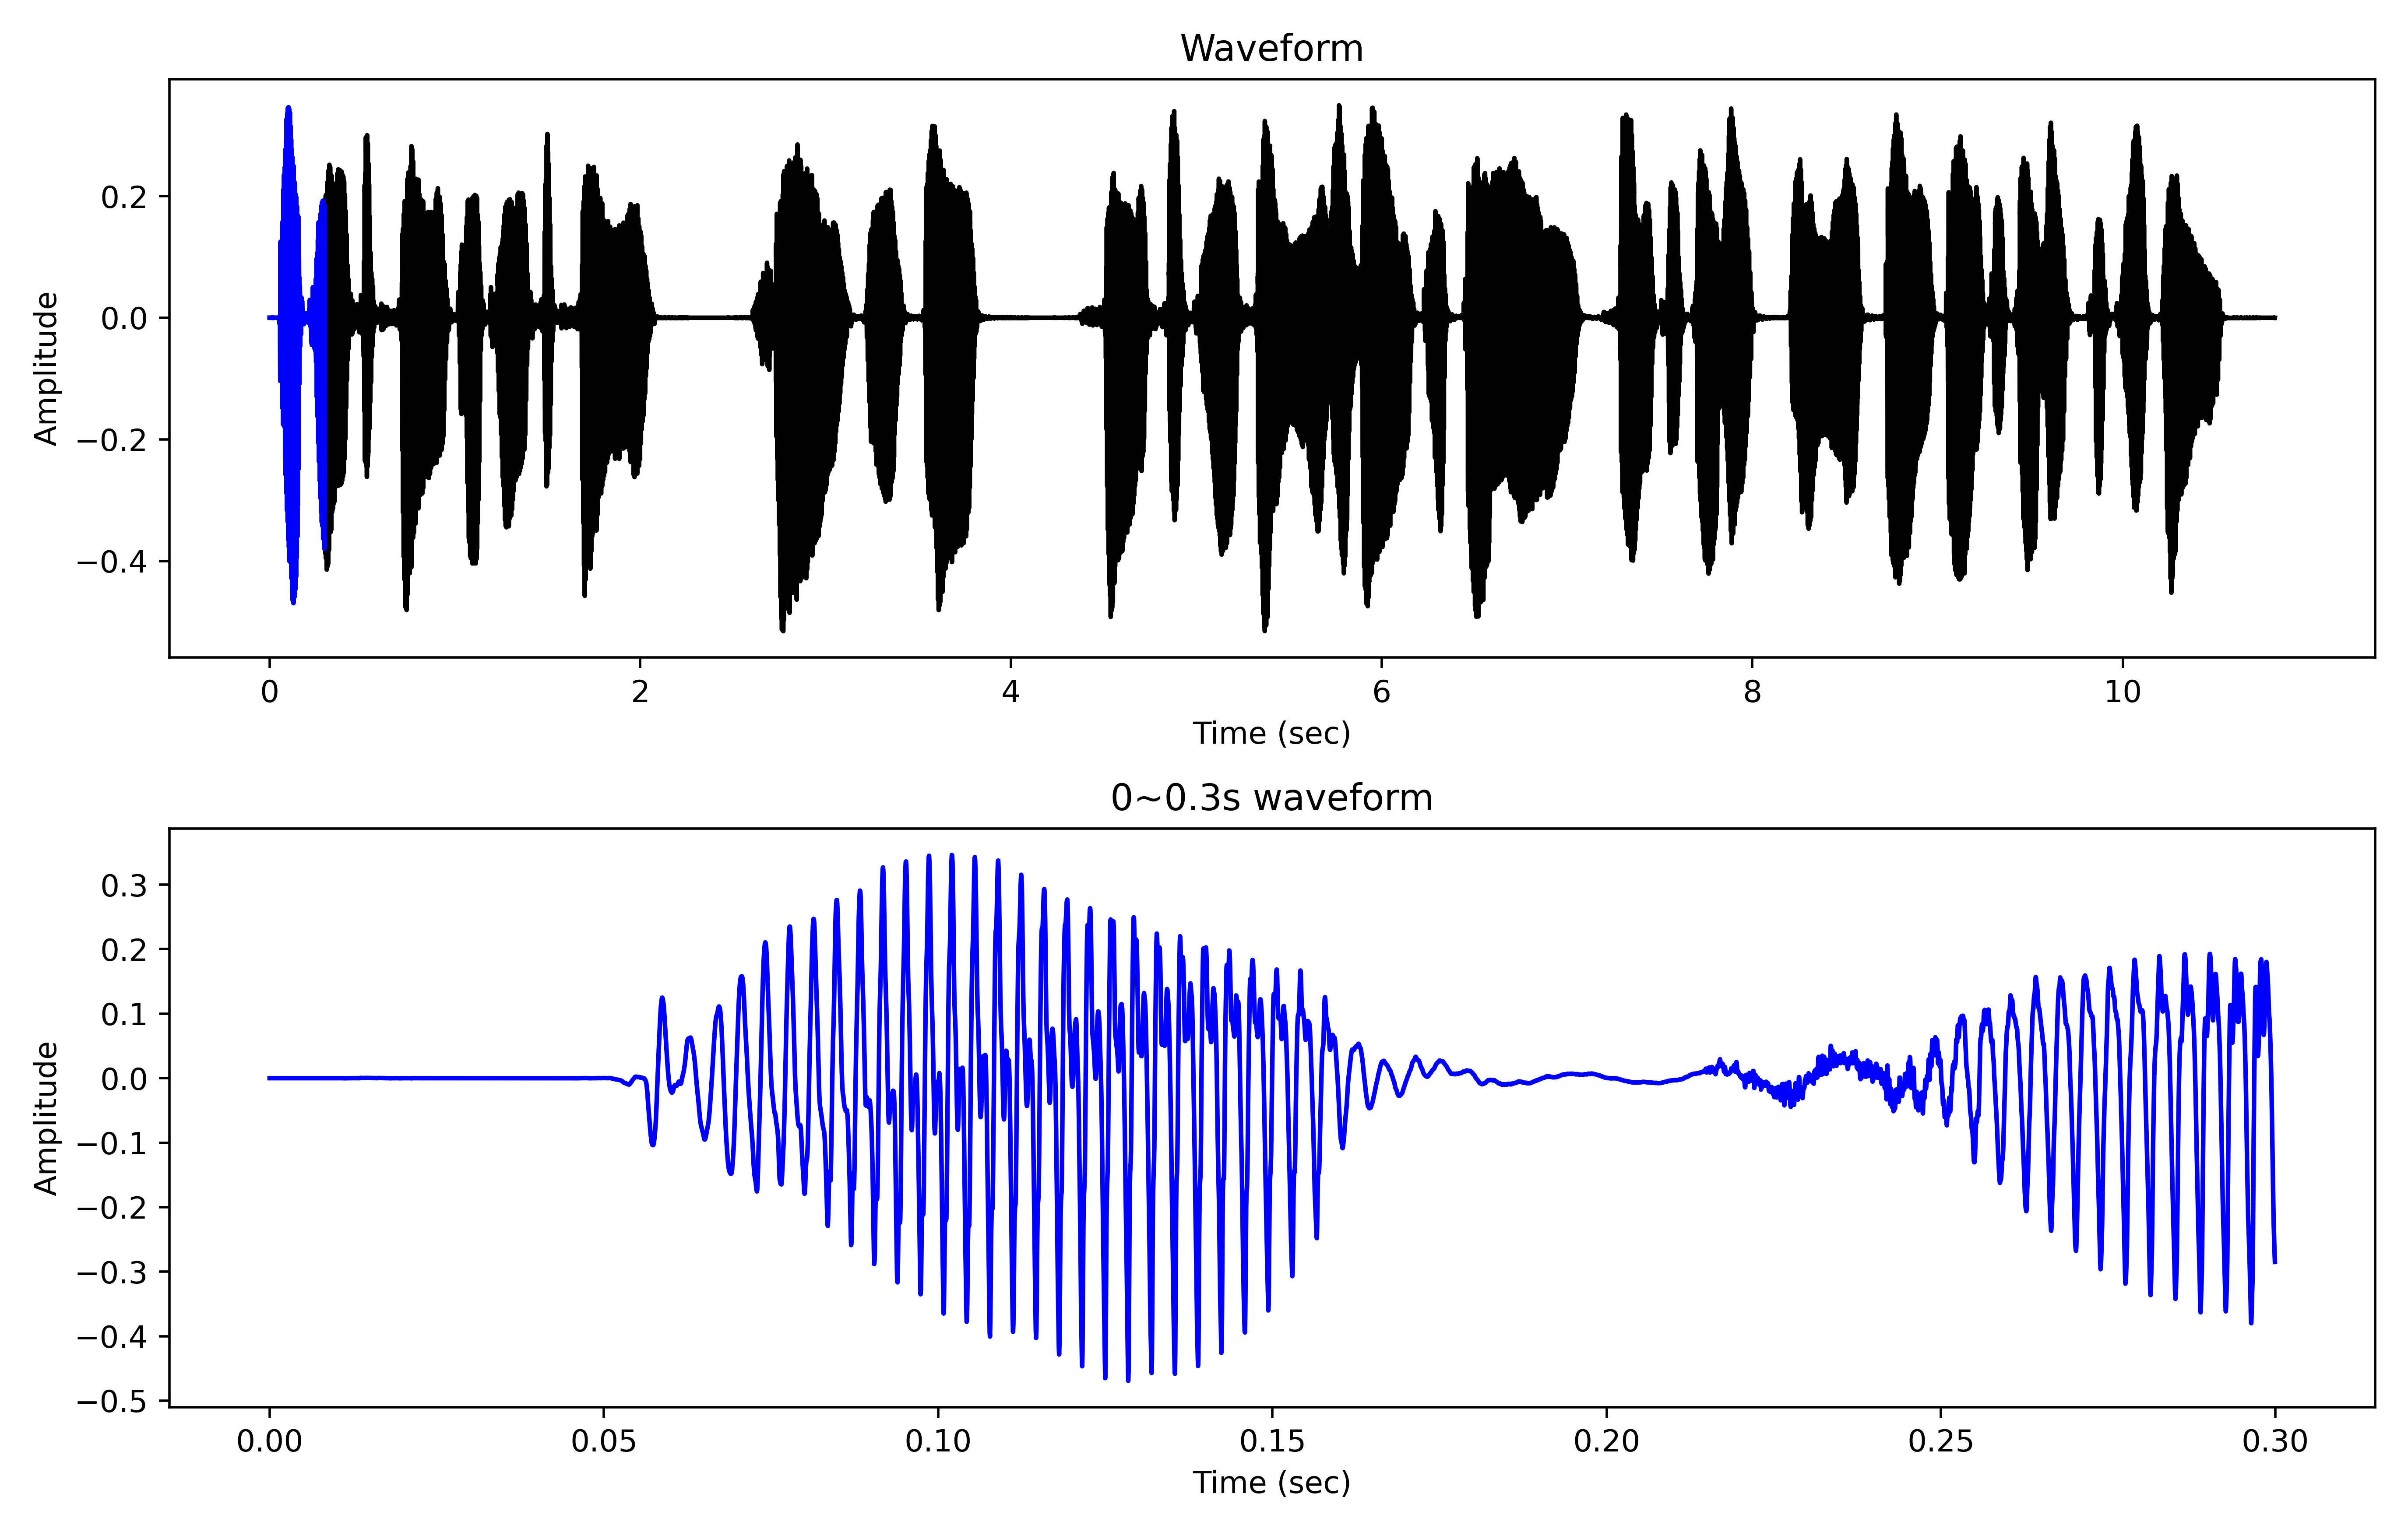
\includegraphics[width=0.6\textwidth]{waveform.png}
  \caption{波形图 \label{fig:waveform}}
\end{figure}


音频有不同的编码类型,librosa默认采取浮点格式读取,即读取的样本点均是 $[-1,-1]$ 之间的浮点值。更详细的文档参见\href{http://sox.sourceforge.net/sox.html}{SoX}的\lstinline{Input & Output File Format Options}部分。

\begin{table}[htbp]
  \centering
  \caption{SoX音频个数}
    \begin{tabular}{llll}
    \toprule
    选项 & 描述 & 常见可选项 \\
    \midrule
    b & 每个编码样本所占的数据位数(位深) & 8/16/32 \\
    c & 音频文件包含的通道数 & 1/2 \\
    e & 音频文件的编码类型 & signed-integer/unsigned-integer/floating-point \\
    r & 音频文件的采样率 & 16k/16000/22050 \\
    t & 音频文件的文件类型 & raw/mp3 \\
    \bottomrule
    \end{tabular}%
\end{table}%

\subsection{提取梅尔频谱}

\begin{lstlisting}
  sample_rate = 16000
  preemphasis = 0.97
  n_fft = 1024
  frame_length = 0.05  # ms
  frame_shift = 0.01  # ms
  fmin = 0
  fmax = sample_rate/2
  eps = 1e-10
  n_mel = 80
  win_length = int(sample_rate*frame_length)
  hop_length = int(sample_rate*frame_shift)
  mel_basis = librosa.filters.mel(
      sample_rate, n_fft, n_mel, fmin=fmin, fmax=fmax)
  
  
  def get_spectrogram(input_wav_path):
      y, sr = librosa.load(input_wav_path)
      y = np.append(y[0], y[1:]-preemphasis*y[:-1])
      linear = librosa.stft(
          y=y, n_fft=n_fft, hop_length=hop_length, win_length=win_length)
      mag = np.abs(linear)
      mel = np.dot(mel_basis, mag)
      mel = np.log10(np.maximum(eps, mel))
      mel = mel.T.astype(np.float32)  # (T,n_mels)
      return mel
  
  # plt.switch_backend('agg')
  
  
  def plot_spectrogram(spectrogram, file_path):
      spectrogram = spectrogram.T
      fig = plt.figure(figsize=(16, 9))
      plt.imshow(spectrogram, aspect='auto', origin='lower')
      plt.colorbar()
      plt.xlabel('frames')
      plt.tight_layout()
      plt.savefig(file_path, dpi=500)
      plt.show()
  
  
  mel_spec = get_spectrogram(input_wav_path)
  plot_spectrogram(mel_spec, 'mel_spectrogram.png')
\end{lstlisting}

\begin{figure}[htbp]
  \centering
  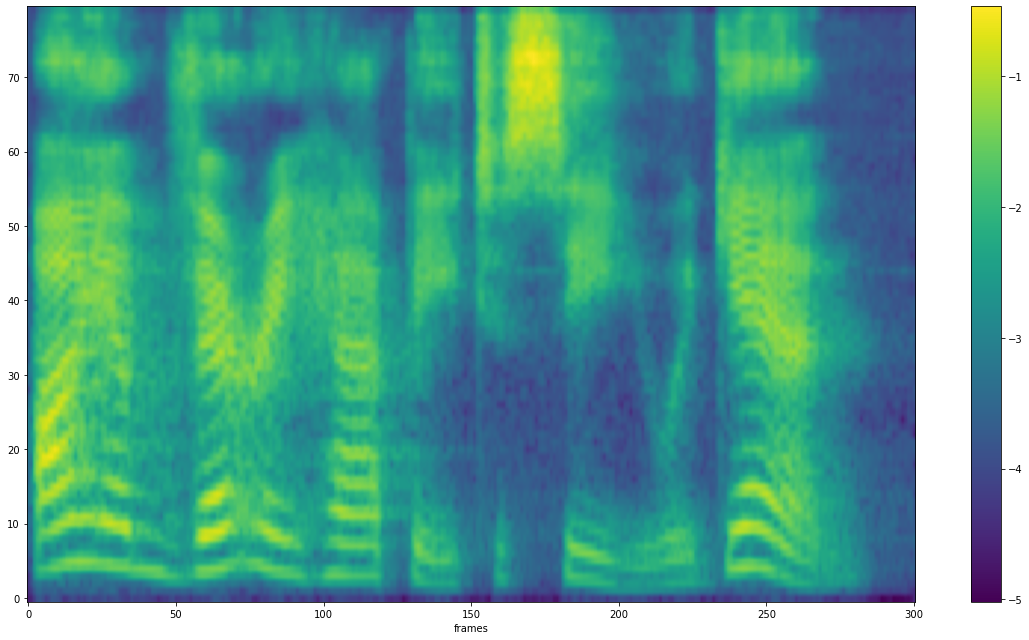
\includegraphics[width=0.6\textwidth]{mel_spectrogram.png}
  \caption{梅尔频谱 \label{fig:mel_spectrogram}}
\end{figure}

\subsection{提取MFCC}

\begin{lstlisting}
  mfcc = dct(mel_spec)
  plot_spectrogram(mfcc, 'mfcc.png')
\end{lstlisting}

\begin{figure}[htbp]
  \centering
  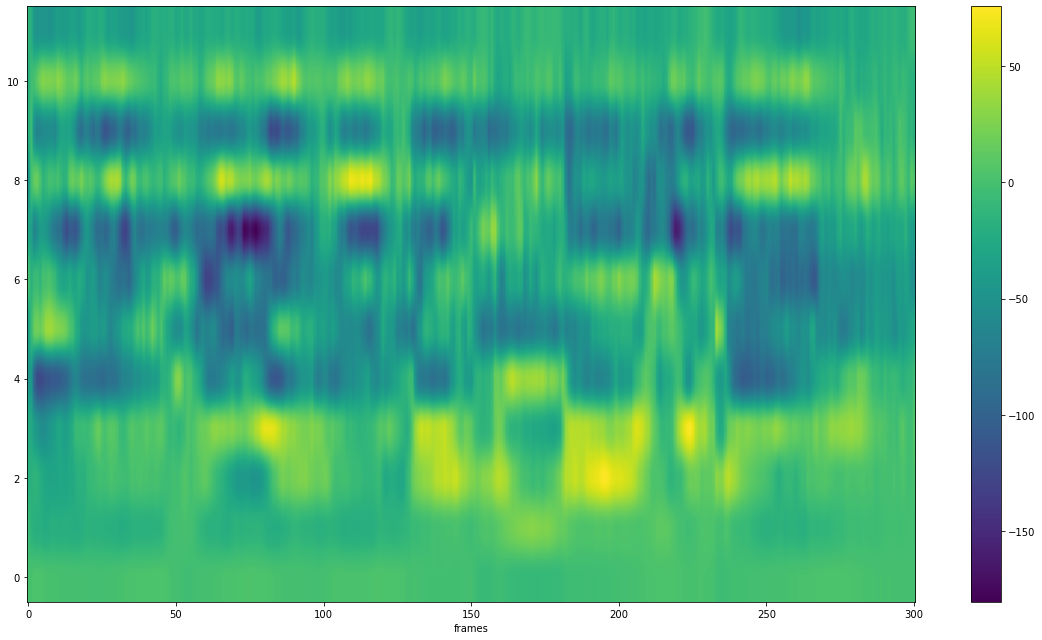
\includegraphics[width=0.6\textwidth]{mfcc.png}
  \caption{MFCC \label{fig:mfcc}}
\end{figure}






\chapter{声学模型}

现代工业级神经网络语音合成系统主要包括三个部分:文本前端、声学模型和声码器,文本输入到文本前端中,将文本转换为音素、韵律边界等文本特征。文本特征输入到声学模型,转换为对应的声学特征。声学特征输入到声码器,重建为原始波形。

\begin{figure}[htbp]
  \centering
  
\includegraphics[width=0.6\textwidth]{text_to_speech-语音合成工作流.png}
  \caption{神经网络TTS的三个主要部件 \label{fig:main_components_in_tts}}
\end{figure}

主要采用的声学模型包括Tacotron系列、FastSpeech系列等,目前同样出现了一些完全端到端的语音合成模型,也即是直接由字符/音素映射为波形。

\section{Tacotron}

以经常使用的Tacotron-2声学模型为例。原始论文参见:

\begin{enumerate}
  \item \href{https://arxiv.org/abs/1703.10135}{Tacotron: Towards End-to-End Speech Synthesis}
  \item \href{https://arxiv.org/abs/1712.05884}{Natural TTS Synthesis by Conditioning WaveNet on Mel Spectrogram Predictions}
\end{enumerate}

此外,谷歌在语音合成领域,特别是端到端语音合成领域做出了开创性的共享,该组会将最新的论文汇总在\href{https://google.github.io/tacotron/}{Tacotron (/täkōˌträn/): An end-to-end speech synthesis system by Google}.

\begin{figure}[htbp]
  \centering
  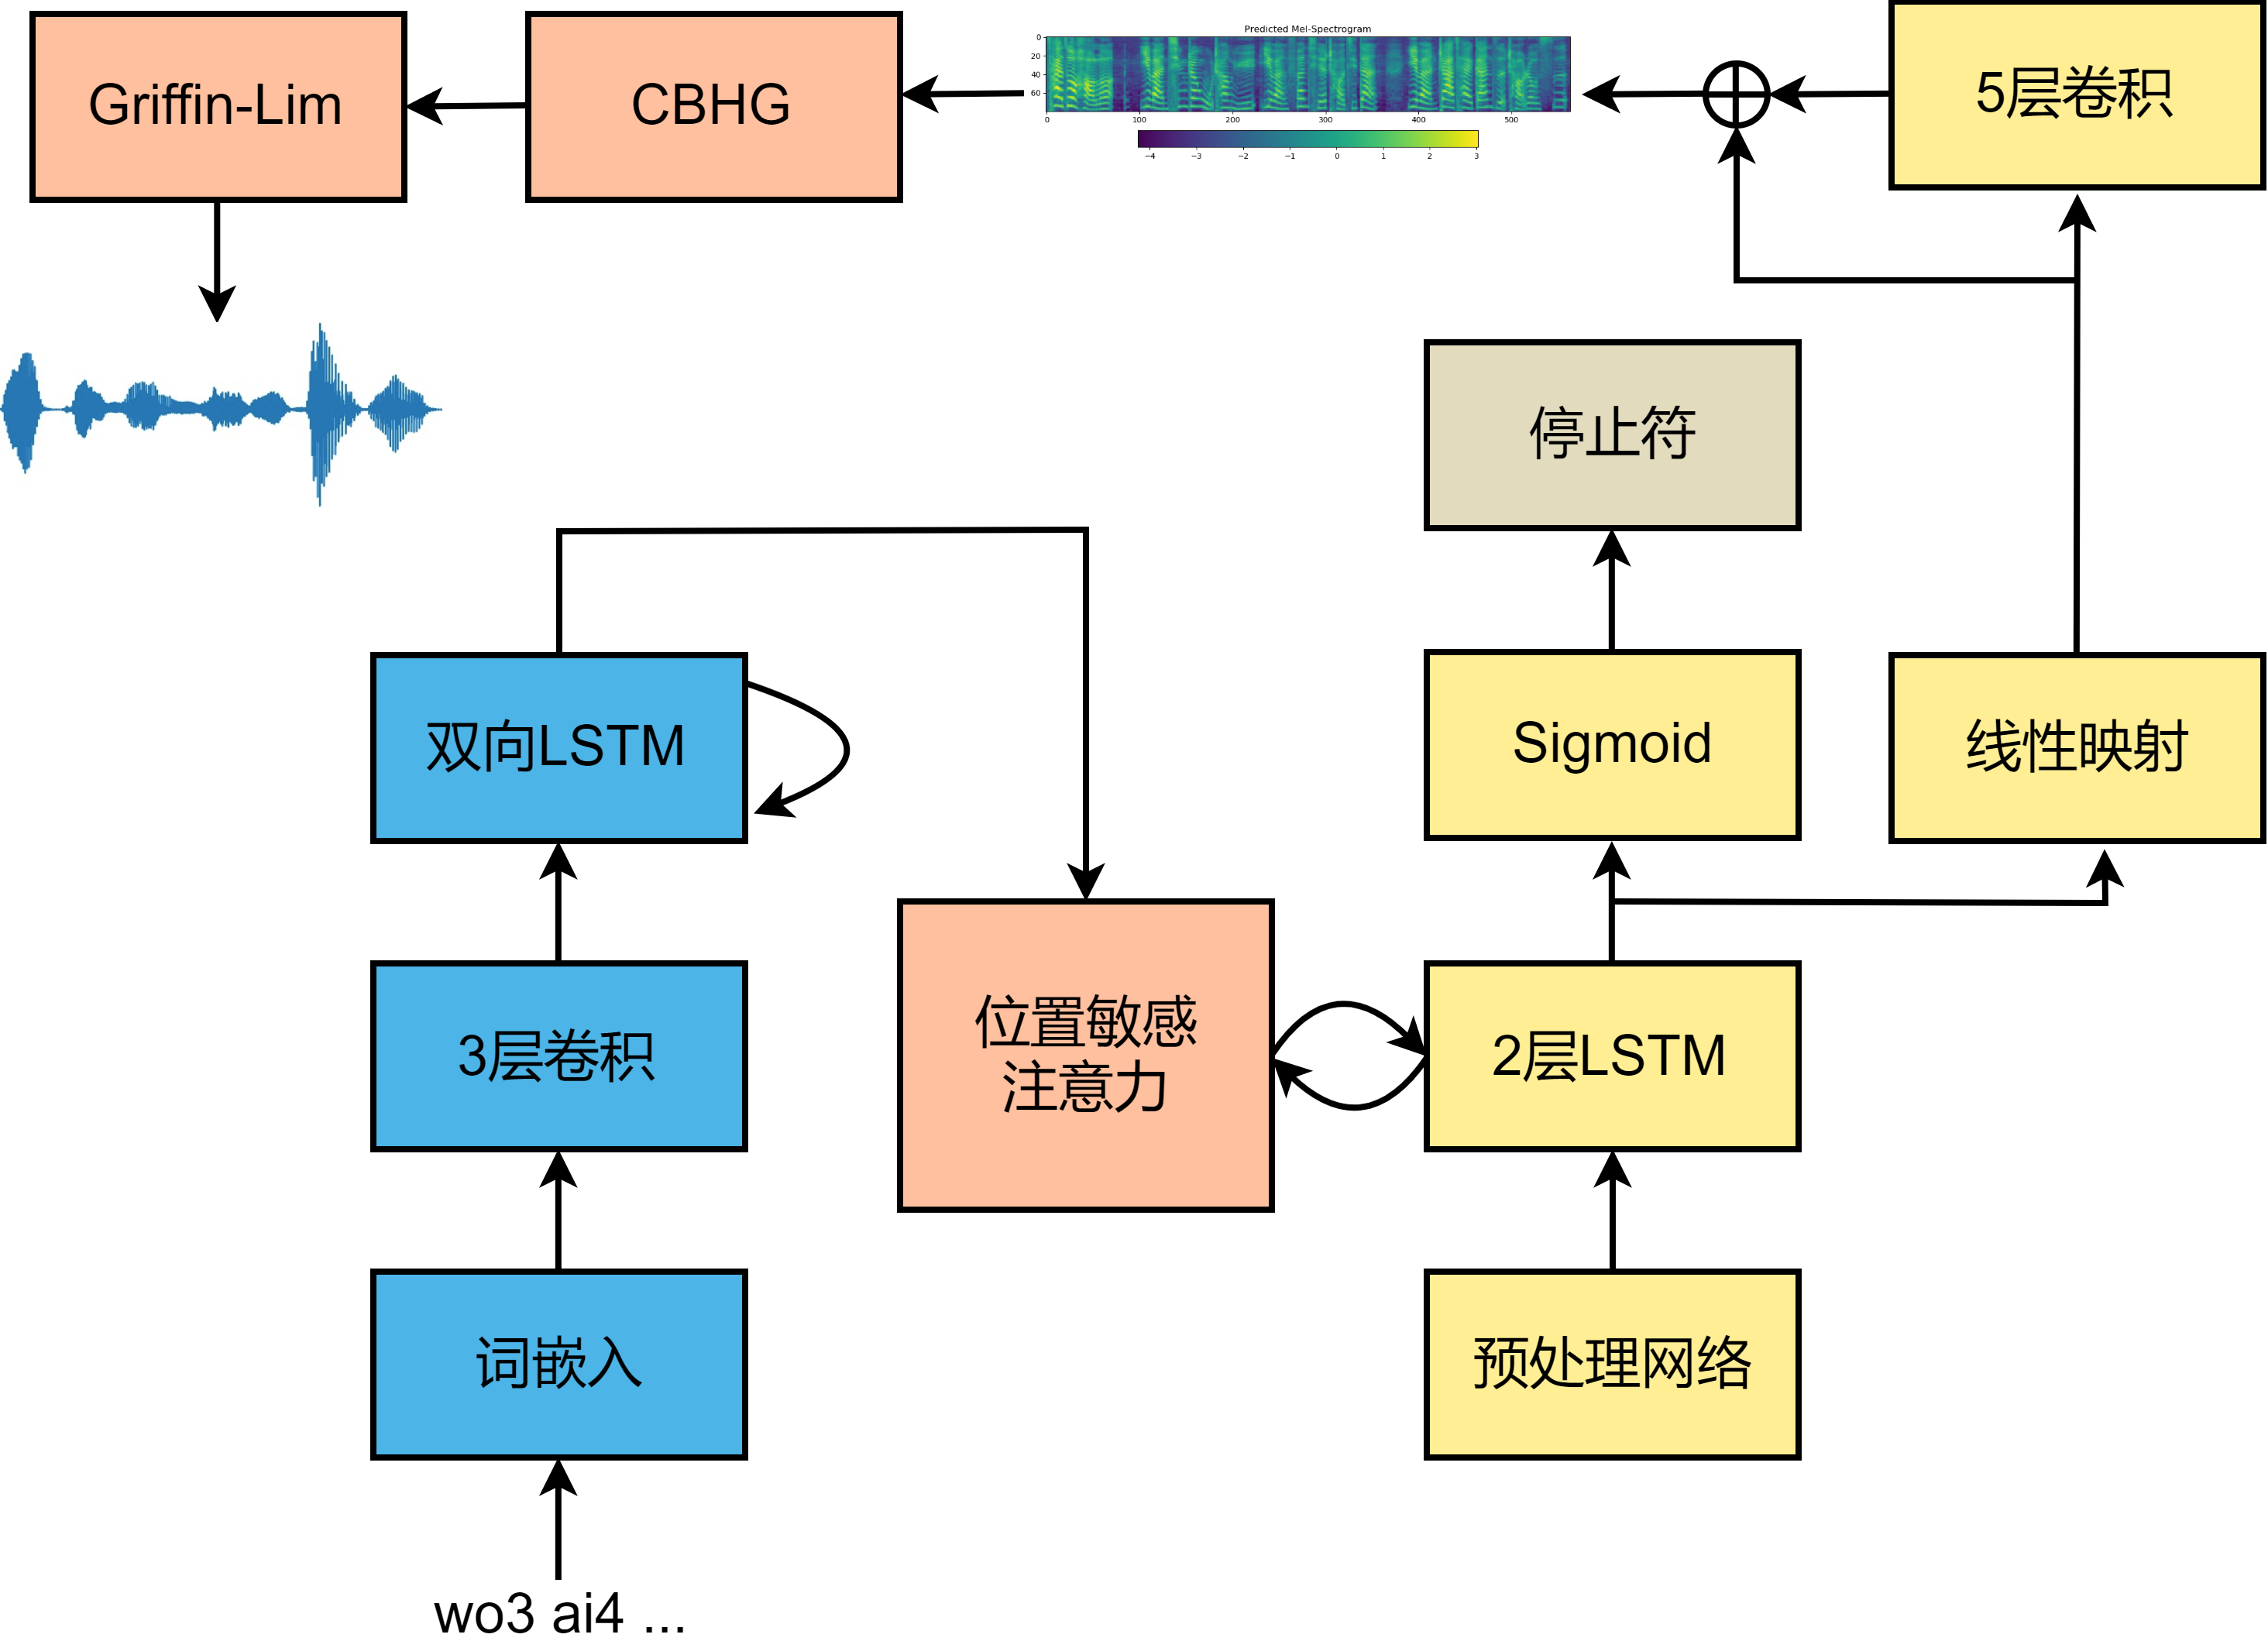
\includegraphics[width=0.6\textwidth]{tacotron2_img.png}
  \caption{Tacotron-2模型结构 \label{fig:tacotron2}}
\end{figure}

Tacotron-2的声学模型部分采用典型的序列到序列结构。编码器是3个卷积层和一个双向LSTM层组成的模块,卷积层给予了模型类似于N-gram感知上下文的能力,并且对不发音字符更加鲁棒。经词嵌入的注音序列首先进入卷积层提取上下文信息,然后送入双向LSTM生成编码器隐状态。编码器隐状态生成后,就会被送入注意力机制,以生成编码向量。我们利用了一种被称为位置敏感注意力(Location Sensitive Attention,LSA),该注意力机制的对齐函数为:

\begin{equation}
  score(s_{i-1},h_j)=v_a^T{\rm tanh}(Ws_{i-1}+Vh_j+Uf_{i,j}+b)
\end{equation}

其中, $v_a,W,V,U$为待训练参数, $b$ 是偏置值, $s_{i-1}$ 为上一时间步 $i-1$ 的解码器隐状态, $h_j$ 为当前时间步 $j$ 的编码器隐状态, $f_{i,j}$ 为上一个解码步的注意力权重 $\alpha_{i-1}$ 经卷积获得的位置特征,如下式:

\begin{equation}
  f_{i,j}=F*\alpha_{i-1}
\end{equation}

其中, $\alpha_{i-1}$ 是经过softmax的注意力权重的累加和。位置敏感注意力机制不但综合了内容方面的信息,而且关注了位置特征。解码过程从输入上一解码步或者真实音频的频谱进入解码器预处理网络开始,到线性映射输出该时间步上的频谱帧结束,模型的解码过程如下图所示。

\begin{figure}[htbp]
  \centering
  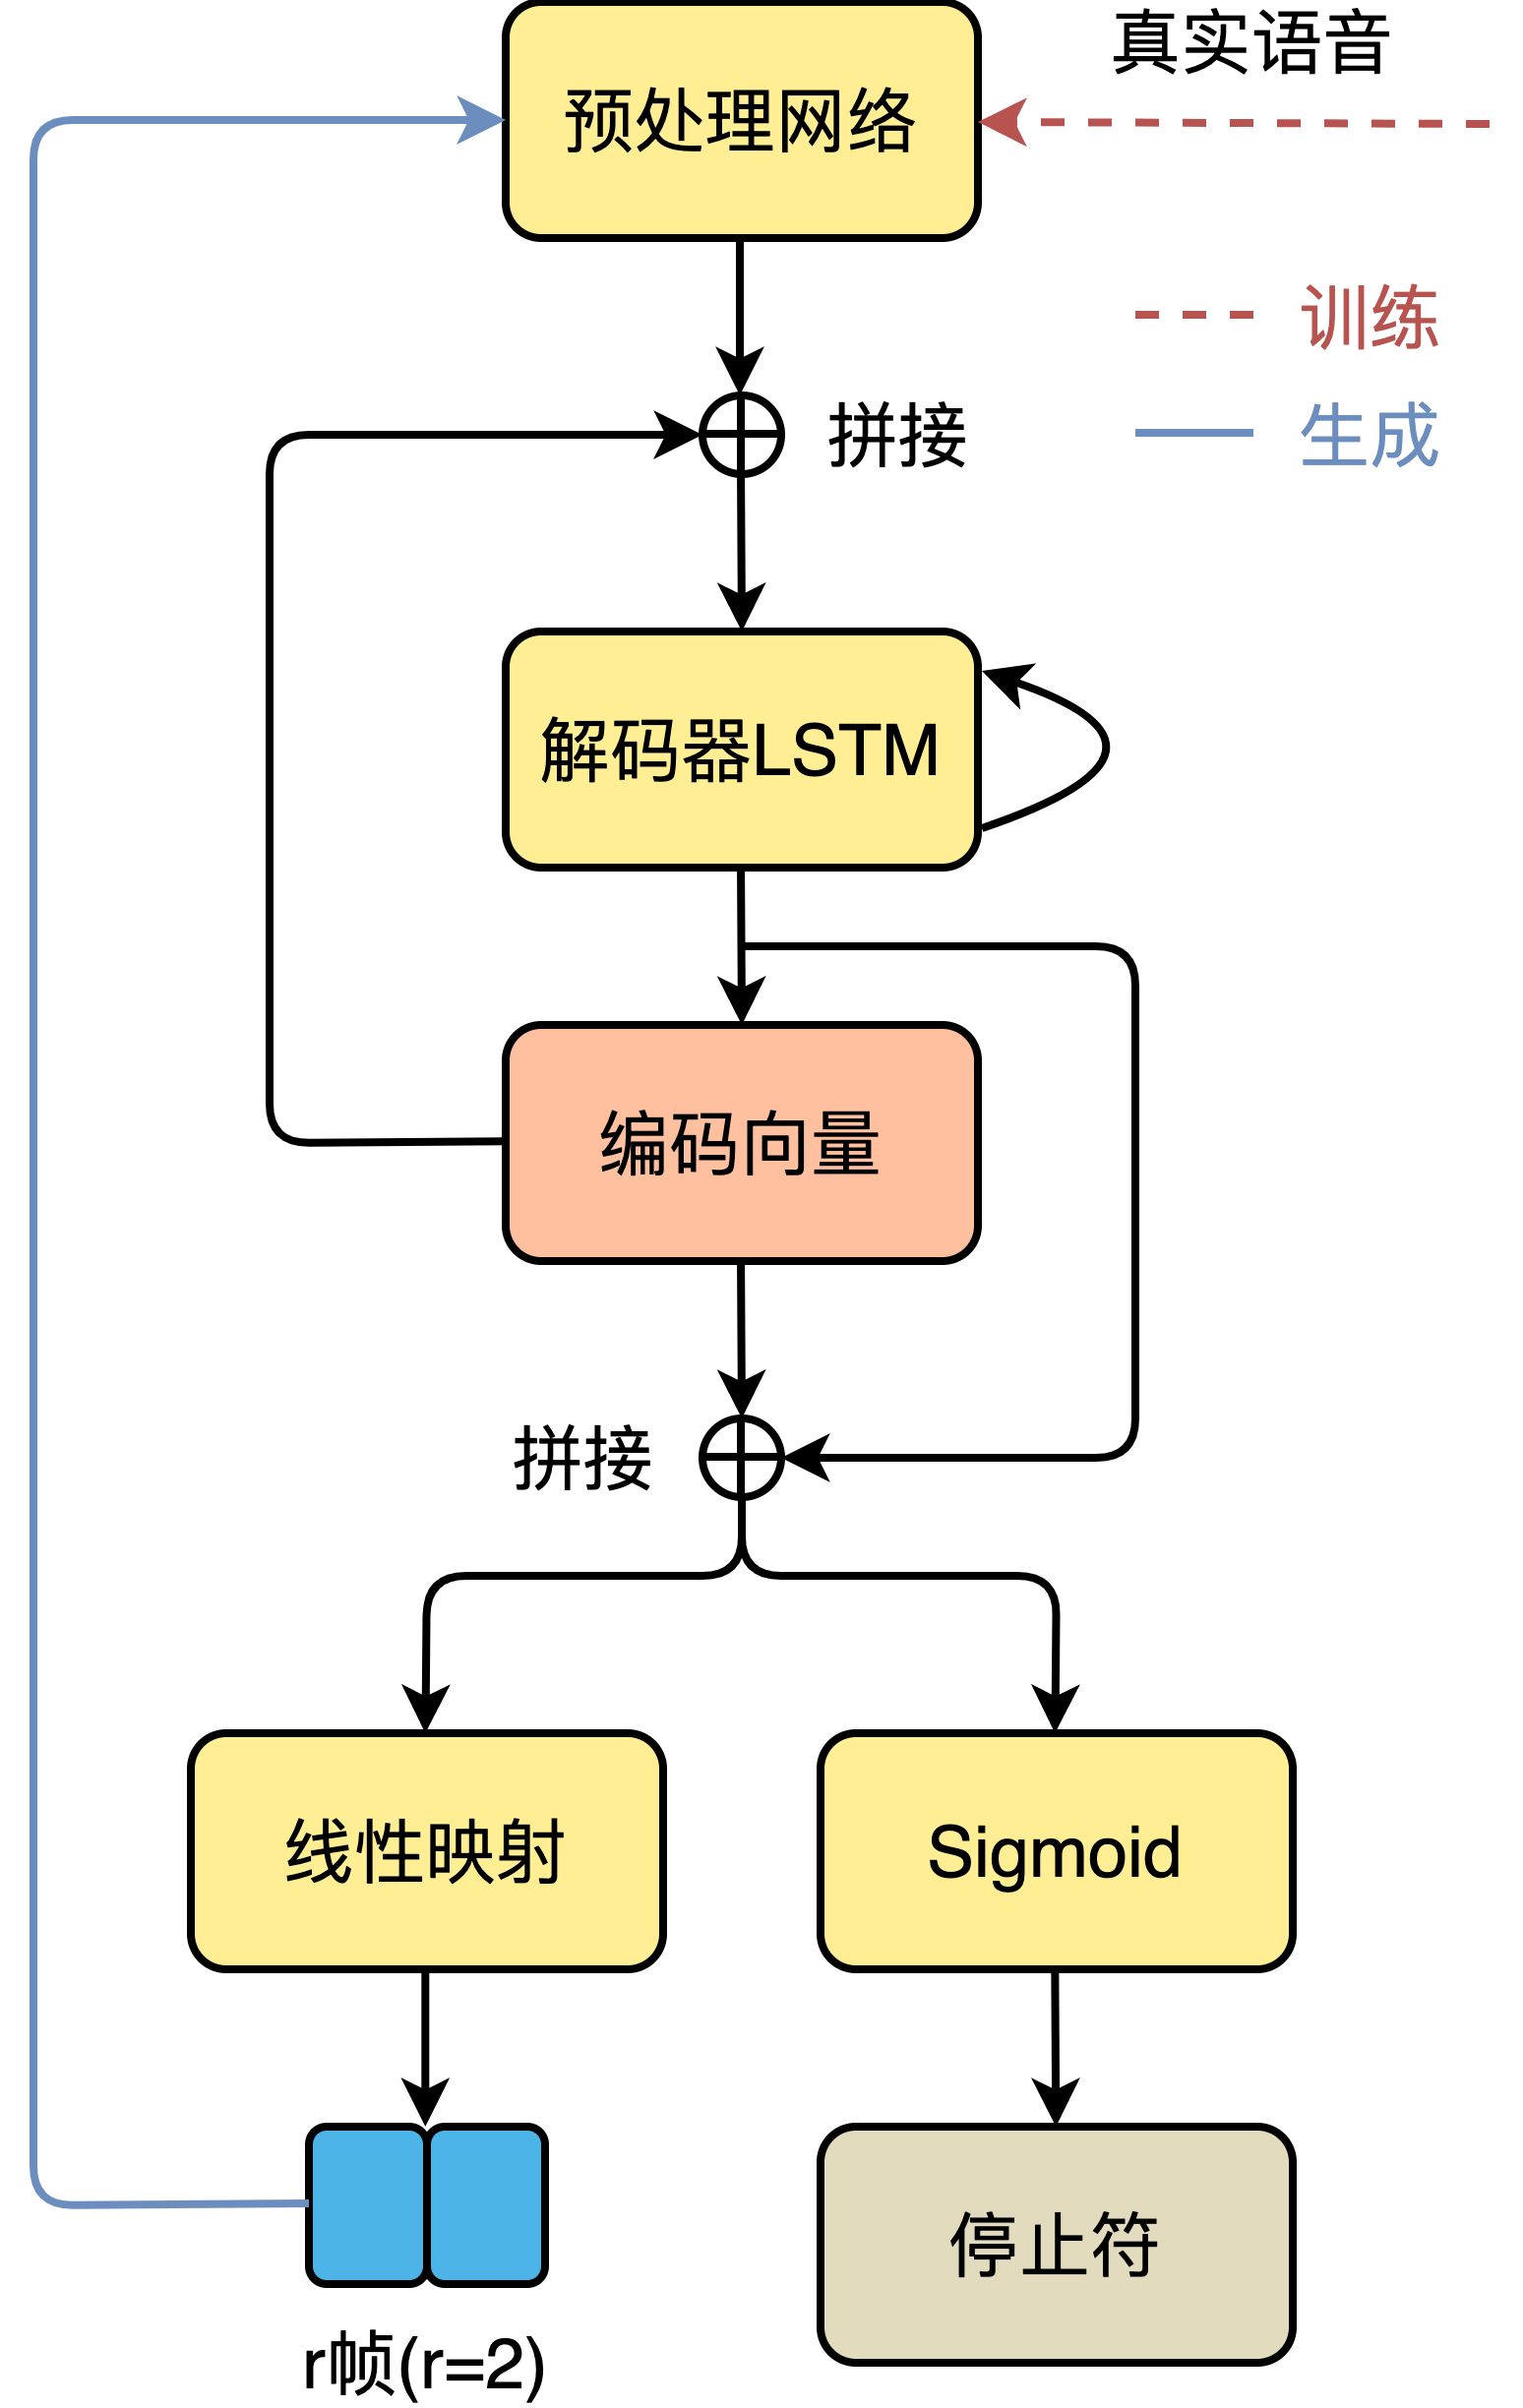
\includegraphics[width=0.6\textwidth]{tacotron2_decoder.png}
  \caption{Tacotron2解码过程 \label{fig:tacotron2_decoder}}
\end{figure}

频谱生成网络的解码器将预处理网络的输出和注意力机制的编码向量做拼接,然后整体送入LSTM中,LSTM的输出用来计算新的编码向量,最后新计算出来的编码向量与LSTM输出做拼接,送入映射层以计算输出。输出有两种形式,一种是频谱帧,另一种是停止符的概率,后者是一个简单二分类问题,决定解码过程是否结束。为了能够有效加速计算,减小内存占用,引入缩减因子r(Reduction Factor),即每一个时间步允许解码器预测r个频谱帧进行输出。解码完成后,送入后处理网络处理以生成最终的梅尔频谱,如下式所示。

\begin{equation}
  s_{final}=s_i+s_i'
\end{equation}

其中, $s_i$ 是解码器输出, $s_{final}$ 表示最终输出的梅尔频谱, $s_i'$ 是后处理网络的输出,解码器的输出经过后处理网络之后获得 $s_i'$ 。

在Tacotron-2原始论文中,直接将梅尔频谱送入声码器WaveNet生成最终的时域波形。但是WaveNet计算复杂度过高,几乎无法实际使用,因此可以使用其它声码器,比如Griffin-Lim、HiFiGAN等。

Tacotron2的损失函数主要包括以下4个方面:

\begin{enumerate}
  \item 进入后处理网络前后的平方损失。
  \begin{equation}
    {\rm MelLoss}=\frac{1}{n}\sum_{i=1}^n(y_{real,i}^{mel}-y_{before,i}^{mel})^2+\frac{1}{n}\sum_{i=1}^n(y_{real,i}^{mel}-y_{after,i}^{mel})^2
  \end{equation}
  其中, $y_{real,i}^{mel}$ 表示从音频中提取的真实频谱, $y_{before,i}^{mel},y_{after,i}^{mel}$ 分别为进入后处理网络前、后的解码器输出, $n$ 为每批的样本数。
  \item 从CBHG模块中输出线性谱的平方损失。
  \begin{equation}
    {\rm LinearLoss}=\frac{1}{n}\sum_{i=1}^{n}(y_{real,i}^{linear}-y_{i}^{linear})^2
  \end{equation}
  其中, $y_{real,i}^{linear}$ 是从真实语音中计算获得的线性谱, $y_{i}^{linear}$ 是从CBHG模块输出的线性谱。
  \item 停止符交叉熵
  \begin{equation}
    {\rm StopTokenLoss}=-[y\cdot {\rm log}(p)+(1-y)\cdot {\rm log}(1-p)]
  \end{equation}
  其中, $y$ 为停止符真实概率分布, $p$ 是解码器线性映射输出的预测分布。
  \item L2正则化
  \begin{equation}
    {\rm RegulationLoss}=\frac{1}{K}\sum_{k=1}^K w_k^2
  \end{equation}
  其中, $K$ 为参数总数, $w_k$ 为模型中的参数,这里排除偏置值、RNN以及线性映射中的参数。最终的损失函数为上述4个部分的损失之和,如下式:
  \begin{equation}
    {\rm Loss}={\rm MelLoss}+{\rm LinearLoss}+{\rm StopTokenLoss}+{\rm RegulationLoss}
  \end{equation}
\end{enumerate}

\section{FastSpeech}

FastSpeech是基于Transformer显式时长建模的声学模型,由微软和浙大提出。原始论文参见:

\begin{enumerate}
  \item \href{https://arxiv.org/abs/1905.09263}{FastSpeech: Fast, Robust and Controllable Text to Speech}
  \item \href{https://arxiv.org/abs/2006.04558}{FastSpeech 2: Fast and High-Quality End-to-End Text to Speech}
\end{enumerate}

相对应地,微软在语音合成领域的论文常常发布在\href{https://speechresearch.github.io/}{Microsoft-Speech Research}。

\begin{figure}[htbp]
  \centering
  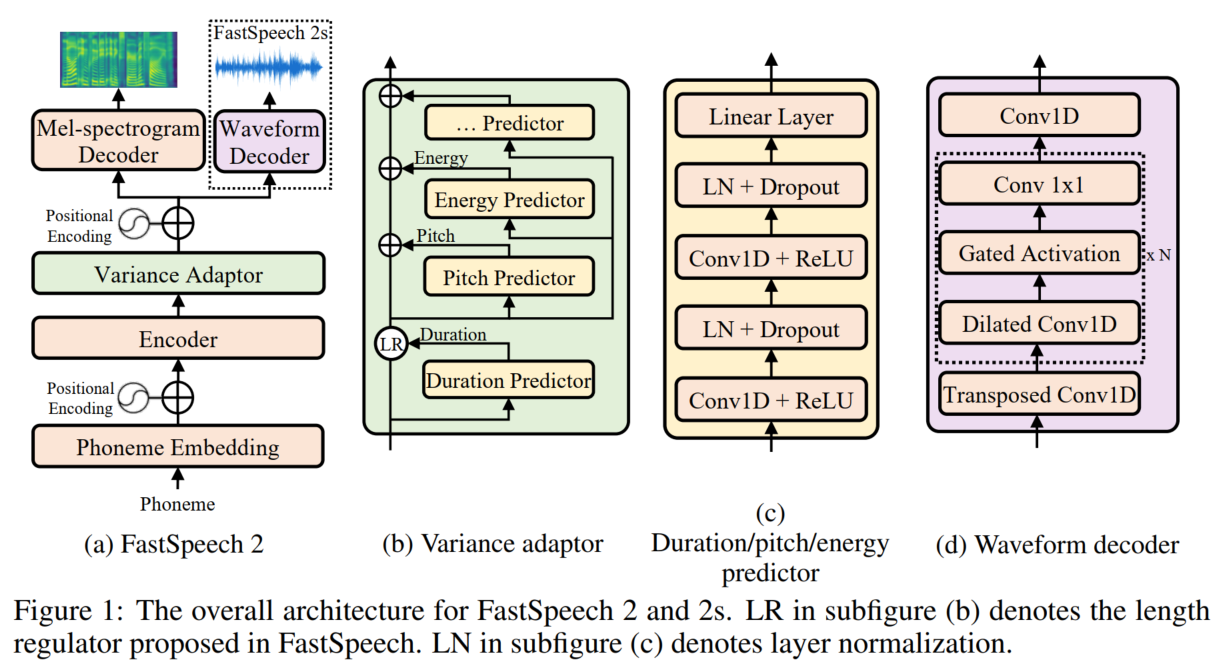
\includegraphics[width=0.6\textwidth]{fastspeech_arch_paper.png}
  \caption{FastSpeech 2整体结构 \label{fig:fastspeech_arch_paper}}
\end{figure}

\subsection{模型结构}

FastSpeech 2和上代FastSpeech的编解码器均是采用FFT(feed-forward Transformer,前馈Transformer)块。编解码器的输入首先进行位置编码,之后进入FFT块。FFT块主要包括多头注意力模块和位置前馈网络,位置前馈网络可以由若干层Conv1d、LayerNorm和Dropout组成。

论文中提到语音合成是典型的一对多问题,同样的文本可以合成无数种语音。上一代FastSpeech主要通过目标侧使用教师模型的合成频谱而非真实频谱,以简化数据偏差,减少语音中的多样性,从而降低训练难度;向模型提供额外的时长信息两个途径解决一对多的问题。在语音中,音素时长自不必说,直接影响发音长度和整体韵律;音调则是影响情感和韵律的另一个特征;能量则影响频谱的幅度,直接影响音频的音量。在FastSpeech 2中对这三个最重要的语音属性单独建模,从而缓解一对多带来的模型学习目标不确定的问题。

在对时长、基频和能量单独建模时,所使用的网络结构实际是相似的,在论文中称这种语音属性建模网络为变量适配器(Variance Adaptor)。时长预测的输出也作为基频和能量预测的输入。最后,基频预测和能量预测的输出,以及依靠时长信息展开的编码器输入元素加起来,作为下游网络的输入。变量适配器主要是由2层卷积和1层线性映射层组成,每层卷积后加ReLU激活、LayerNorm和Dropout。代码摘抄自\href{https://github.com/ming024/FastSpeech2}{FastSpeech2},添加了一些注释。

\begin{lstlisting}
class VariancePredictor(nn.Module):
  """ Duration, Pitch and Energy Predictor """
  def __init__(self):
      super(VariancePredictor, self).__init__()

      self.input_size = hp.encoder_hidden
      self.filter_size = hp.variance_predictor_filter_size
      self.kernel = hp.variance_predictor_kernel_size
      self.conv_output_size = hp.variance_predictor_filter_size
      self.dropout = hp.variance_predictor_dropout

      self.conv_layer = nn.Sequential(OrderedDict([
          ("conv1d_1", Conv(self.input_size,
                            self.filter_size,
                            kernel_size=self.kernel,
                            padding=(self.kernel-1)//2)),
          ("relu_1", nn.ReLU()),
          ("layer_norm_1", nn.LayerNorm(self.filter_size)),
          ("dropout_1", nn.Dropout(self.dropout)),
          ("conv1d_2", Conv(self.filter_size,
                            self.filter_size,
                            kernel_size=self.kernel,
                            padding=1)),
          ("relu_2", nn.ReLU()),
          ("layer_norm_2", nn.LayerNorm(self.filter_size)),
          ("dropout_2", nn.Dropout(self.dropout))
      ]))

      self.linear_layer = nn.Linear(self.conv_output_size, 1)

  def forward(self, encoder_output, mask):
      '''
      :param encoder_output: Output of encoder. [batch_size,seq_len,encoder_hidden]
      :param mask: Mask for encoder. [batch_size,seq_len]
      '''
      out = self.conv_layer(encoder_output)
      out = self.linear_layer(out)
      out = out.squeeze(-1)

      if mask is not None:
          out = out.masked_fill(mask, 0.)

      return out
\end{lstlisting}

利用该变量适配器对时长、基频和能量进行建模。

\begin{lstlisting}
class VarianceAdaptor(nn.Module):
  """ Variance Adaptor """

  def __init__(self):
      super(VarianceAdaptor, self).__init__()
      self.duration_predictor = VariancePredictor()
      self.length_regulator = LengthRegulator()
      self.pitch_predictor = VariancePredictor()
      self.energy_predictor = VariancePredictor()

      self.pitch_bins = nn.Parameter(torch.exp(torch.linspace(
          np.log(hp.f0_min), np.log(hp.f0_max), hp.n_bins-1)), requires_grad=False)
      self.energy_bins = nn.Parameter(torch.linspace(
          hp.energy_min, hp.energy_max, hp.n_bins-1), requires_grad=False)
      self.pitch_embedding = nn.Embedding(hp.n_bins, hp.encoder_hidden)
      self.energy_embedding = nn.Embedding(hp.n_bins, hp.encoder_hidden)

  def forward(self, x, src_mask, mel_mask=None, duration_target=None, pitch_target=None, energy_target=None, max_len=None, d_control=1.0, p_control=1.0, e_control=1.0):
      '''
      :param x: Output of encoder. [batch_size,seq_len,encoder_hidden]
      :param src_mask: Mask of encoder, can get src_mask form input_lengths. [batch_size,seq_len]
      :param duration_target, pitch_target, energy_target: Ground-truth when training, None when synthesis. [batch_size,seq_len]
      '''
      log_duration_prediction = self.duration_predictor(x, src_mask)
      if duration_target is not None:
          x, mel_len = self.length_regulator(x, duration_target, max_len)
      else:
          duration_rounded = torch.clamp(
              (torch.round(torch.exp(log_duration_prediction)-hp.log_offset)*d_control), min=0)
          x, mel_len = self.length_regulator(x, duration_rounded, max_len)
          mel_mask = utils.get_mask_from_lengths(mel_len)

      pitch_prediction = self.pitch_predictor(x, mel_mask)
      if pitch_target is not None:
          pitch_embedding = self.pitch_embedding(
              torch.bucketize(pitch_target, self.pitch_bins))
      else:
          pitch_prediction = pitch_prediction*p_control
          pitch_embedding = self.pitch_embedding(
              torch.bucketize(pitch_prediction, self.pitch_bins))

      energy_prediction = self.energy_predictor(x, mel_mask)
      if energy_target is not None:
          energy_embedding = self.energy_embedding(
              torch.bucketize(energy_target, self.energy_bins))
      else:
          energy_prediction = energy_prediction*e_control
          energy_embedding = self.energy_embedding(
              torch.bucketize(energy_prediction, self.energy_bins))

      x = x + pitch_embedding + energy_embedding

      return x, log_duration_prediction, pitch_prediction, energy_prediction, mel_len, mel_mask
\end{lstlisting}

同样是通过长度调节器(Length Regulator),利用时长信息将编码器输出长度扩展到频谱长度。具体实现就是根据duration的具体值,直接上采样。一个音素时长为2,就将编码器输出复制2份,给3就直接复制3份,拼接之后作为最终的输出。实现代码:

\begin{lstlisting}
class LengthRegulator(nn.Module):
  """ Length Regulator """

  def __init__(self):
      super(LengthRegulator, self).__init__()

  def LR(self, x, duration, max_len):
      '''
      :param x: Output of encoder. [batch_size,phoneme_seq_len,encoder_hidden]
      :param duration: Duration for phonemes. [batch_size,phoneme_seq_len]
      :param max_len: Max length for mel-frames. scaler

      Return:
      output: Expanded output of encoder. [batch_size,mel_len,encoder_hidden]
      '''
      output = list()
      mel_len = list()
      for batch, expand_target in zip(x, duration):
          # batch: [seq_len,encoder_hidden]
          # expand_target: [seq_len]
          expanded = self.expand(batch, expand_target)
          output.append(expanded)
          mel_len.append(expanded.shape[0])

      if max_len is not None:
          output = utils.pad(output, max_len)
      else:
          output = utils.pad(output)

      return output, torch.LongTensor(mel_len).to(device)

  def expand(self, batch, predicted):
      out = list()

      for i, vec in enumerate(batch):
          # expand_size: scaler
          expand_size = predicted[i].item()
          # Passing -1 as the size for a dimension means not changing the size of that dimension.
          out.append(vec.expand(int(expand_size), -1))
      out = torch.cat(out, 0)

      return out

  def forward(self, x, duration, max_len):
      output, mel_len = self.LR(x, duration, max_len)
      return output, mel_len
\end{lstlisting}

对于音高和能量的预测,模块的主干网络相似,但使用方法有所不同。以音高为例,能量的使用方式相似。首先对预测出的实数域音高值进行分桶,映射为一定范围内的自然数集,然后做嵌入。

\begin{lstlisting}
pitch_prediction = self.pitch_predictor(x, mel_mask)
if pitch_target is not None:
  pitch_embedding = self.pitch_embedding(
      torch.bucketize(pitch_target, self.pitch_bins))
else:
  pitch_prediction = pitch_prediction*p_control
  pitch_embedding = self.pitch_embedding(
      torch.bucketize(pitch_prediction, self.pitch_bins))
\end{lstlisting}

这里用到了Pytorch中一个不是特别常见的函数\href{https://pytorch.org/docs/master/generated/torch.bucketize.html}{torch.bucketize}。这是Pytorch中的分桶函数,boundaries确定了各个桶的边界,是一个单调递增向量,用于划分input,并返回input所属桶的索引,桶索引从0开始。

能量嵌入向量的计算方法与之类似。至此,获得了展开之后的编码器输出x,基频嵌入向量\lstinline{pitch_embedding}和能量嵌入向量\lstinline{energy_embedding}之后,元素加获得最终编解码器的输入。

\subsection{损失函数}

FastSpeech 2的目标函数由PostNet前后的频谱均方差,时长、音高和能量的均方差组成。时长映射到指数域(时长预测器输出的数值 $x$ 作为指数,最终的预测时长为 $e^x$ ),音高映射到对数域(音高预测器输出的数值 $x$ 做对数,作为最终的音高 ${\rm log} x$ ),而能量直接采用能量预测器的输出值。整体的损失函数为:

\begin{equation}
  {\rm Loss}={\rm Loss}_{mel}+{\rm Loss}_{mel}^{post}+{\rm Loss}_{duration}+{\rm Loss}_{pitch}+{\rm Loss}_{energy}
\end{equation}

频谱的损失函数形式采用均方差(MSE),时长、基频和能量采用平均绝对误差(MAE),具体的实现如下:

\begin{lstlisting}
log_d_target.requires_grad = False
p_target.requires_grad = False
e_target.requires_grad = False
mel_target.requires_grad = False

log_d_predicted = log_d_predicted.masked_select(src_mask)
log_d_target = log_d_target.masked_select(src_mask)
p_predicted = p_predicted.masked_select(mel_mask)
p_target = p_target.masked_select(mel_mask)
e_predicted = e_predicted.masked_select(mel_mask)
e_target = e_target.masked_select(mel_mask)

mel = mel.masked_select(mel_mask.unsqueeze(-1))
mel_postnet = mel_postnet.masked_select(mel_mask.unsqueeze(-1))
mel_target = mel_target.masked_select(mel_mask.unsqueeze(-1))

mel_loss = self.mse_loss(mel, mel_target)
mel_postnet_loss = self.mse_loss(mel_postnet, mel_target)

d_loss = self.mae_loss(log_d_predicted, log_d_target)
p_loss = self.mae_loss(p_predicted, p_target)
e_loss = self.mae_loss(e_predicted, e_target)

total_loss = mel_loss + mel_postnet_loss + d_loss + p_loss + e_loss
\end{lstlisting}

\subsection{小结}

FastSpeech系列的声学模型将Transformer引入语音合成领域,并且显式建模语音中的重要特征,比如时长、音高和能量等。实际上,微软首次在\href{https://arxiv.org/abs/1809.08895}{Neural Speech Synthesis with Transformer Network}将Transformer作为主干网络,实现语音合成的声学模型,这一思想同样被\href{https://arxiv.org/abs/2006.06873}{FastPitch: Parallel Text-to-speech with Pitch Prediction}采用,相关的开源代码:\href{https://github.com/as-ideas/TransformerTTS}{as-ideas/TransformerTTS}。

\section{VITS}

VITS(Variational Inference with adversarial learning for end-to-end Text-to-Speech)是一种结合变分推理(variational inference)、标准化流(normalizing flows)和对抗训练的高表现力语音合成模型。和Tacotron和FastSpeech不同,Tacotron / FastSpeech实际是将字符或音素映射为中间声学表征,比如梅尔频谱,然后通过声码器将梅尔频谱还原为波形,而VITS则直接将字符或音素映射为波形,不需要额外的声码器重建波形,真正的端到端语音合成模型。VITS通过隐变量而非之前的频谱串联语音合成中的声学模型和声码器,在隐变量上进行建模并利用随机时长预测器,提高了合成语音的多样性,输入同样的文本,能够合成不同声调和韵律的语音。VITS合成音质较高,并且可以借鉴之前的FastSpeech,单独对音高等特征进行建模,以进一步提升合成语音的质量,是一种非常有潜力的语音合成模型。

\subsection{模型整体结构}

\begin{figure}[htbp]
  \centering
  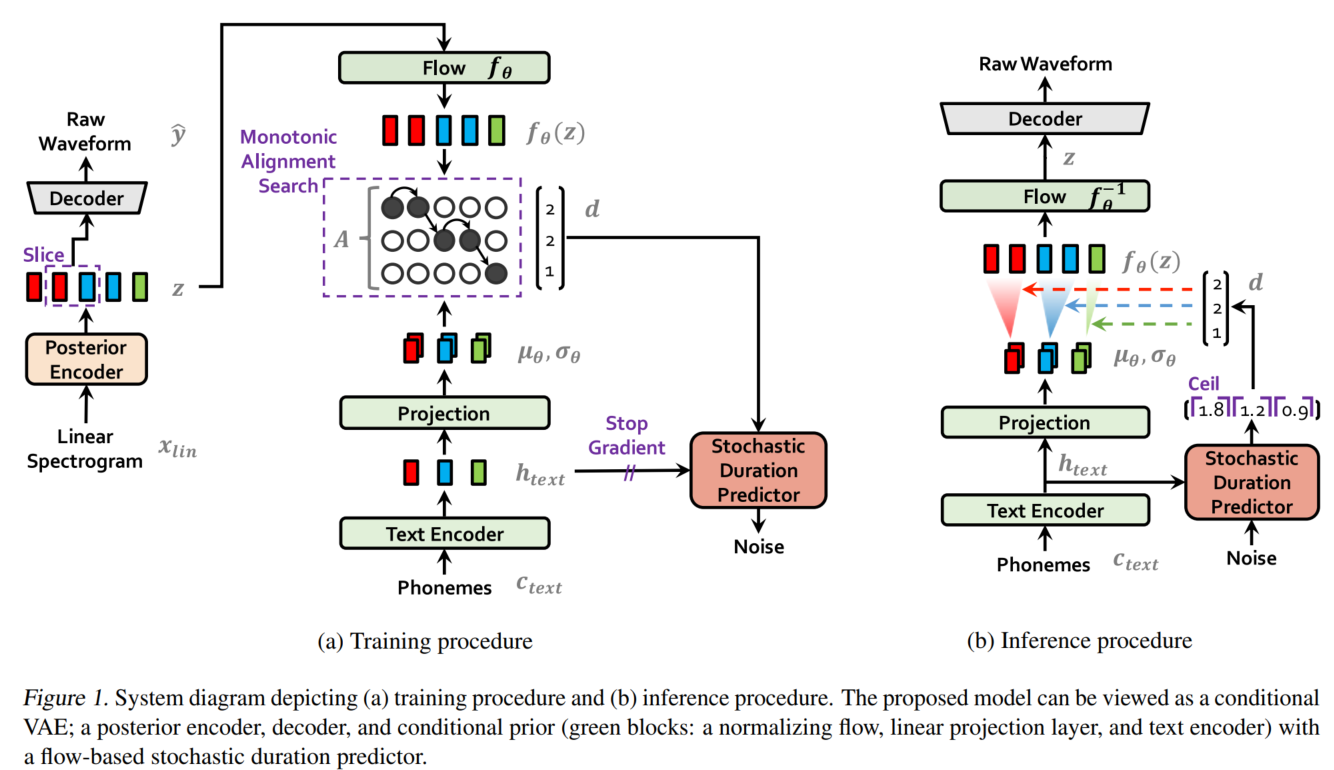
\includegraphics[width=0.6\textwidth]{vits_arch.png}
  \caption{VITS整体结构 \label{fig:vits_arch}}
\end{figure}

VITS包括三个部分:

\begin{enumerate}
  \item 后验编码器。如上图(a)的左下部分所示,在训练时输入线性谱,输出隐变量 $z$ ,推断时隐变量 $z$ 则由 $f_\theta$ 产生。VITS的后验编码器采用WaveGlow和Glow-TTS中的非因果WaveNet残差模块。应用于多人模型时,将说话人嵌入向量添加进残差模块,\lstinline{仅用于训练}。这里的隐变量 $z$ 可以理解为Tacotron / FastSpeech中的梅尔频谱。
  \item 解码器。如上图(a)左上部分所示,解码器从提取的隐变量 $z$ 中生成语音波形,这个解码器实际就是声码器HiFi-GAN V1的生成器。应用于多人模型时,在说话人嵌入向量之后添加一个线性层,拼接到 $f_\theta$ 的输出隐变量 $z$ 。
  \item 先验编码器。如上图(a)右侧部分所示,先验编码器结构比较复杂,作用类似于Tacotron / FastSpeech的声学模型,只不过VITS是将音素映射为中间表示 $z$ ,而不是将音素映射为频谱。包括文本编码器和提升先验分布复杂度的标准化流 $f_\theta$ 。应用于多人模型时,向标准化流的残差模块中添加说话人嵌入向量。
  \item 随机时长预测器。如上图(a)右侧中间橙色部分。从条件输入 $h_{text}$ 估算音素时长的分布。应用于多人模型时,在说话人嵌入向量之后添加一个线性层,并将其拼接到文本编码器的输出 $h_{text}$ 。
  \item 判别器。实际就是HiFi-GAN的多周期判别器,在上图中未画出,\lstinline{仅用于训练}。目前看来,对于任意语音合成模型,加入判别器辅助都可以显著提升表现。
\end{enumerate}

\subsection{变分推断}

VITS可以看作是一个最大化变分下界,也即ELBO(Evidence Lower Bound)的条件VAE。

\begin{enumerate}
  \item 重建损失
  
  VITS在训练时实际还是会生成梅尔频谱以指导模型的训练,重建损失中的目标使用的是梅尔频谱而非原始波形:
  \begin{equation}
    {\rm L}_{recon}=||x_{mel}-\hat{x}_{mel}||_1
  \end{equation}
  但在推断时并不需要生成梅尔频谱。在实现上,不上采样整个隐变量 $z$ ,而只是使用部分序列作为解码器的输入。

  \item KL散度
  
  先验编码器 $c$ 的输入包括从文本生成的音素 $c_{text}$ ,和音素、隐变量之间的对齐 $A$ 。所谓的对齐就是 $|c_{text}|\times |z|$ 大小的严格单调注意力矩阵,表示每一个音素的发音时长。因此KL散度是:
  \begin{equation}
    {\rm L}_{kl}={\rm log}q_{\phi}(z|x_{lin})-{\rm log}p_\theta (z|c_{text},A)
  \end{equation}
  其中, $q_{\phi}(z|x_{lin})$ 表示给定输入 $x$ 的后验分布, $p_\theta(z|c)$ 表示给定条件 $c$ 的隐变量 $z$ 的先验分布。其中隐变量 $z$ 为:
  \begin{equation}
    z\sim q_\phi(z|x_{lin})=\mathbb{N}(z;\mu_\phi(x_{lin}),\sigma_\phi(x_{lin}))
  \end{equation}
  为了给后验编码器提供更高分辨率的信息,使用线性谱而非梅尔频谱作为后验编码器 $\phi_\theta$ 的输入。同时,为了生成更加逼真的样本,提高先验分布的表达能力比较重要,因此引入标准化流,在文本编码器产生的简单分布和复杂分布间进行可逆变换。也就是说,在经过上采样的编码器输出之后,加入一系列可逆变换:
  \begin{equation}
    p_\theta(z|c)=\mathbb{N}(f_\theta(z);\mu_\theta(c),\sigma_\theta(c))|{\rm det}\frac{\partial f_\theta(z)}{\partial z}|
  \end{equation}
  其中,上式中的 $c$ 就是上采样的编码器输出:
  \begin{equation}
    c=[c_{text},A]
  \end{equation}
\end{enumerate}


\subsection{对齐估计}

由于在训练时没有对齐的真实标签,因此在训练的每一次迭代时都需要估计对齐。

\begin{enumerate}
  \item 单调对齐搜索
  
  为了估计文本和语音之间的对齐 $A$ ,VITS采用了类似于Glow-TTS中的单调对齐搜索(Monotonic Alignment Search,MAS)方法,该方法寻找一个最优的对齐路径以最大化利用标准化流 $f$ 参数化数据的对数似然:
  \begin{equation}
    A=\underset{\hat{A}}{\rm argmax}{\rm log}p(x|c_{text},\hat{A})=\underset{\hat{A}}{\rm argmax}{\rm log}\mathbb{N}(f(x);\mu(c_{text},\hat{A}),\sigma(c_{text},\hat{A}))
  \end{equation}
  MAS约束获得的最优对齐必须是单调且无跳过的。但是无法直接将MAS直接应用到VITS,因为VITS优化目标是ELBO而非确定的隐变量 $z$ 的对数似然,因此稍微改变了一下MAS,寻找最优的对齐路径以最大化ELBO:
  \begin{equation}
    \underset{\hat{A}}{\rm argmax}{\rm log}p_\theta (x_{mel}|z)-{\rm log}\frac{q_\theta(z|x_{lin})}{p_\theta (z|c_{text},\hat{A})}
  \end{equation}

  \item 随机时长预测器
  
  随机时长预测器是一个基于流的生成模型,训练目标为音素时长对数似然的变分下界:
  \begin{equation}
    {\rm log}p_\theta (d|c_{text}\geq \mathbb{E}_{q_\theta (u,v|d,c_{text})}[{\rm log}\frac{p_\theta (d-u,v|c_{text})}{q_\phi (u,v|d,c_{text})}]
  \end{equation}
  在训练时,断开随机时长预测器的梯度反传,以防止该部分的梯度影响到其它模块。音素时长通过随机时长预测器的可逆变换从随机噪音中采样获得,之后转换为整型值。

\end{enumerate}

\subsection{对抗训练}

引入判别器 $D$ 判断输出是解码器 $G$ 的输出,还是真实的波形 $y$ 。VITS用于对抗训练的损失函数包括两个部分,第一部分是用于对抗训练的最小二乘损失函数(least-squares loss function): 

\begin{equation}
  {\rm L}_{adv}(D)=\mathbb{E}_{(y,z)}[(D(y)-1)^2+(D(G(z)))^2]
\end{equation}

\begin{equation}
  {\rm L}_{adv}(G)=\mathbb{E}_z[(D(G(z))-1)^2]
\end{equation}

第二部分是仅作用于生成器的特征匹配损失(feature-matching loss):

\begin{equation}
  {\rm L}_{fm}(G)=\mathbb{E}_{(y,c)}[\sum_{l=1}^T\frac{1}{N_l}||D^l(y)-D^l(G(z))||_1]
\end{equation}

其中, $T$ 表示判别器的层数, $D^l$ 表示第 $l$ 层判别器的特征图(feature map), $N_l$ 表示特征图的数量。特征匹配损失可以看作是重建损失,用于约束判别器中间层的输出。

\subsection{总体损失}

VITS可以看作是VAE和GAN的联合训练,因此总体损失为:

\begin{equation}
  {\rm L}_{vae}={\rm L}_{recon}+{\rm L}_{kl}+{\rm L}_{dur}+{\rm L}_{adv}+{\rm L}_{fm}(G)
\end{equation}

\subsection{总结}

VITS是一种由字符或音素直接映射为波形的端到端语音合成模型,该语音合成模型采用对抗训练的模式,生成器多个模块基于标准化流。模型较大,合成质量优异。VITS的想法相当有启发,但是理解起来确实比较难,特别是标准化流,可参考:\href{https://github.com/janosh/awesome-normalizing-flows}{Awesome Normalizing Flows}。




% 声码器部分
\chapter{声码器}

声码器(Vocoder),又称语音信号分析合成系统,负责对声音进行分析和合成,主要用于合成人类的语音。声码器主要由以下功能:

\begin{enumerate}
  \item 分析Analysis
  \item 操纵Manipulation
  \item 合成Synthesis
\end{enumerate}

分析过程主要是从一段原始声音波形中提取声学特征,比如线性谱、MFCC;操纵过程是指对提取的原始声学特征进行压缩等降维处理,使其表征能力进一步提升;合成过程是指将此声学特征恢复至原始波形。人类发声机理可以用经典的源-滤波器模型建模,也就是输入的激励部分通过线性时不变进行操作,输出的声道谐振部分作为合成语音。输入部分被称为激励部分(Source Excitation Part),激励部分对应肺部气流与声带共同作用形成的激励,输出结果被称为声道谐振部分(Vocal Tract Resonance Part),对应人类发音结构,而声道谐振部分对应于声道的调音部分,对声音进行调制。

声码器的发展可以分为两个阶段,包括用于统计参数语音合成(Statistical Parameteric Speech Synthesis,SPSS)基于信号处理的声码器,和基于神经网络的声码器。常用基于信号处理的声码器包括Griffin-Lim\footnote{Griffin D. and Lim J. (1984). "Signal Estimation from Modified Short-Time Fourier Transform". IEEE Transactions on Acoustics, Speech and Signal Processing. 32 (2): 236–243. doi:10.1109/TASSP.1984.1164317},STRAIGHT\footnote{Kawahara H. Speech representation and transformation using adaptive interpolation of weighted spectrum: vocoder revisited[C]. 1997 IEEE International Conference on Acoustics, Speech, and Signal Processing. IEEE, 1997, 2: 1303-1306.}和WORLD\footnote{Morise M, Yokomori F, Ozawa K. World: a vocoder-based high-quality speech synthesis system for real-time applications[J]. IEICE TRANSACTIONS on Information and Systems, 2016, 99(7): 1877-1884.}。早期神经声码器包括WaveNet、WaveRNN等,近年来神经声码器发展迅速,涌现出包括MelGAN、HiFiGAN、LPCNet、NHV等优秀的工作。

\section{Griffin-Lim声码器}

在早期的很多Tacotron开源语音合成模型中均采用Griffin-Lim声码器,同时也有一些专门的开源实现,比如\href{https://github.com/bkvogel/griffin_lim}{GriffinLim}。

\subsection{算法原理}

原始的音频很难提取特征,需要进行傅里叶变换将时域信号转换到频域进行分析。音频进行傅里叶变换后,结果为复数,复数的绝对值就是幅度谱,而复数的实部与虚部之间形成的角度就是相位谱。经过傅里叶变换之后获得的幅度谱特征明显,可以清楚看到基频和对应的谐波。基频一般是声带的频率,而谐波则是声音经过声道、口腔、鼻腔等器官后产生的共振频率,且频率是基频的整数倍。

Griffin-Lim将幅度谱恢复为原始波形,但是相比原始波形,幅度谱缺失了原始相位谱信息。音频一般采用的是短时傅里叶变化,因此需要将音频分割成帧(每帧20ms~50ms),再进行傅里叶变换,帧与帧之间是有重叠的。Griffin-Lim算法利用两帧之间有重叠部分的这个约束重构信号,因此如果使用Griffin-Lim算法还原音频信号,就需要尽量保证两帧之间重叠越多越好,一般帧移为每一帧长度的25\%左右,也就是帧之间重叠75\%为宜。

Griffin-Lim在已知幅度谱,不知道相位谱的情况下重建语音,算法的实现较为简单,整体是一种迭代算法,迭代过程如下:

\begin{enumerate}
  \item 随机初始化一个相位谱;
  \item 用相位谱和已知的幅度谱经过逆短时傅里叶变换(ISTFT)合成新语音;
  \item 对合成的语音做短时傅里叶变换,得到新的幅度谱和相位谱;
  \item 丢弃新的幅度谱,用相位谱和已知的幅度谱合成语音,如此重复,直至达到设定的迭代轮数。
\end{enumerate}

在迭代过程中,预测序列与真实序列幅度谱之间的距离在不断缩小,类似于EM算法。推导过程参见:\href{https://zhuanlan.zhihu.com/p/102539783}{Griffin Lim算法的过程和证明}和\href{https://zhuanlan.zhihu.com/p/66809424}{Griffin Lim声码器介绍}。


\subsection{代码实现}

摘抄自\href{https://zhuanlan.zhihu.com/p/25002923}{Build End-To-End TTS Tacotron: Griffin Lim 信号估计算法}。

\begin{lstlisting}
def griffin_lim(stftm_matrix, shape, min_iter=20, max_iter=50, delta=20):
  y = np.random.random(shape)
  y_iter = []

  for i in range(max_iter):
      if i >= min_iter and (i - min_iter) % delta == 0:
          y_iter.append((y, i))
      stft_matrix = librosa.core.stft(y)
      stft_matrix = stftm_matrix * stft_matrix / np.abs(stft_matrix)
      y = librosa.core.istft(stft_matrix)
  y_iter.append((y, max_iter))

  return y_iter
\end{lstlisting}

具体使用:

\begin{lstlisting}
# assume 1 channel wav file
sr, data = scipy.io.wavfile.read(input_wav_path)

# 由 STFT -> STFT magnitude
stftm_matrix = np.abs(librosa.core.stft(data))
# + random 模拟 modification
stftm_matrix_modified = stftm_matrix + np.random.random(stftm_matrix.shape)

# Griffin-Lim 估计音频信号
y_iters = griffin_lim(stftm_matrix_modified, data.shape)
\end{lstlisting}


\section{STRAIGHT声码器}

\subsection{概述}

STARIGHT(Speech Transformation and Representation using Adaptive Interpolation of weiGHTed spectrum),即利用自适应加权谱内插进行语音转换和表征。STRAIGHT将语音信号解析成相互独立的频谱参数(谱包络)和基频参数(激励部分),能够对语音信号的基频、时长、增益、语速等参数进行灵活的调整,该模型在分析阶段仅针对语音基音、平滑功率谱和非周期成分3个声学参数进行分析提取,在合成阶段利用上述3个声学参数进行语音重构。

STRAIGHT采用源-滤波器表征语音信号,可将语音信号看作激励信号通过时变线性滤波器的结果。

\begin{note}
  对于能量信号和周期信号,其傅里叶变换收敛,因此可以用频谱(Spectrum)来描述;对于随机信号,傅里叶变换不收敛,因此不能用频谱进行描述,而应当使用功率谱(PSD),不严谨地说,功率谱可以看作是随机信号的频谱,参见\href{https://zhuanlan.zhihu.com/p/417454806}{功率谱密度(PSD)}。
\end{note}

\subsection{特征提取}

\begin{enumerate}
  \item 平滑功率谱的提取,包括低频带补偿和清音帧处理等过程。STRAIGHT分析阶段的一个关键步骤是进行自适应频谱分析,获取无干扰且平滑的功率谱。自适应加权谱的提取关键在于对提取出来的功率谱进行一系列的平滑和补偿。对输入信号进行:语音信号预处理->功率谱提取->低频噪声补偿->过平滑补偿->静音帧谱图的处理,最后得到自适应功率谱。
  \item 非周期成分提取。
  \item 通过小波时频分析的方式,提取基频轨迹。首先通过对语音信号中的基频信息进行解析,然后计算出相应的瞬时基频值,最后在频域进行谐波解析,并在频率轴进行平滑处理,获得语音信号的各个基频参数。
\end{enumerate}

\subsection{语音合成}

STARIGHT采用PSOLA技术和最小相位脉冲响应相结合的方式,在合成语音时输入待合成语音的基音频率轨迹和去除了周期性的二维短时谱包络。

开源的STRAIGHT声码器大多是MATLAB实现,比如\href{https://github.com/HidekiKawahara/legacy_STRAIGHT}{Legacy STRAIGHT},\href{https://github.com/ashmanmode/StraightRepo}{StraightRepo}。在开源语音合成系统\href{https://github.com/CSTR-Edinburgh/merlin}{merlin}中存在可用的STRAIGHT工具,参见\href{https://github.com/CSTR-Edinburgh/merlin/blob/master/misc/scripts/vocoder/straight/copy_synthesis.sh}{StraightCopySynthesis}。

\section{WORLD声码器}

\subsection{声学特征}

WORLD通过获取三个声学特征合成原始语音,这三个声学特征分别是:基频(fundamental frequency,F0),频谱包络(Spectrum Envelop,也称频谱参数Spectrum Parameter,SP)和非周期信号参数(Aperiodic Parameter,AP)。

\begin{enumerate}
  \item 基频F0
  
  基频F0决定浊音,对应激励部分的周期脉冲序列,如果将声学信号分为周期和非周期信号,基频F0部分包含了语音的韵律信息和结构信息。对于一个由振动而发出的声音信号,这个信号可以看作是若干组频率不同的正弦波叠加而成,其中频率最低的正弦波即为\lstinline{基频},其它则为\lstinline{泛音}。

  WORLD提取基频的流程:首先,利用低通滤波器对原始信号进行滤波;之后,对滤波之后的信号进行评估,由于滤波之后的信号应该恰好是一个正弦波,每个波段的长度应该恰好都是一个周期长度,因此通过计算这四个周期的标准差,可以评估此正弦波正确与否;最后选取标准差最小周期的倒数作为最终的基频。

  \item 频谱包络SP
  
  频谱包络SP决定音色,对应声道谐振部分时不变系统的冲激响应,可以看作通过此线性时不变系统之后,声码器会对激励与系统响应进行卷积。将不同频率的振幅最高点通过平滑的曲线连接起来,就是频谱包络,求解方法有多种,在求解梅尔倒谱系数时,使用的是倒谱法。

  \begin{note}
    倒频谱(Cepstrum)也称为倒谱、二次谱和对数功率谱等,倒频谱的工程定义为:信号功率谱对数值进行傅里叶逆变换的结果,也就是:信号->求功率谱->求对数->求傅里叶逆变换。参见\href{https://zhuanlan.zhihu.com/p/34989414}{信号频域分析方法的理解(频谱、能量谱、功率谱、倒频谱、小波分析)}。
  \end{note}

  \item 非周期信号参数AP
  
  非周期信号参数AP决定清音,对应混合激励部分的非周期脉冲序列,一般的语音都是由周期和非周期信号组成,因此除了上述的周期信号的声学参数,还需要非周期信号参数,才能够恢复出原始信号。混合激励可以通过AP来控制浊音段中周期激励和噪音(非周期)成分的相对比重。

\end{enumerate}

\subsection{WORLD的分析功能}

WORLD包含3个语音分析模块,语音分析模型包括DIO模块、CheapTrick模块,PLATINUM模块。

\begin{figure}[htbp]
  \centering
  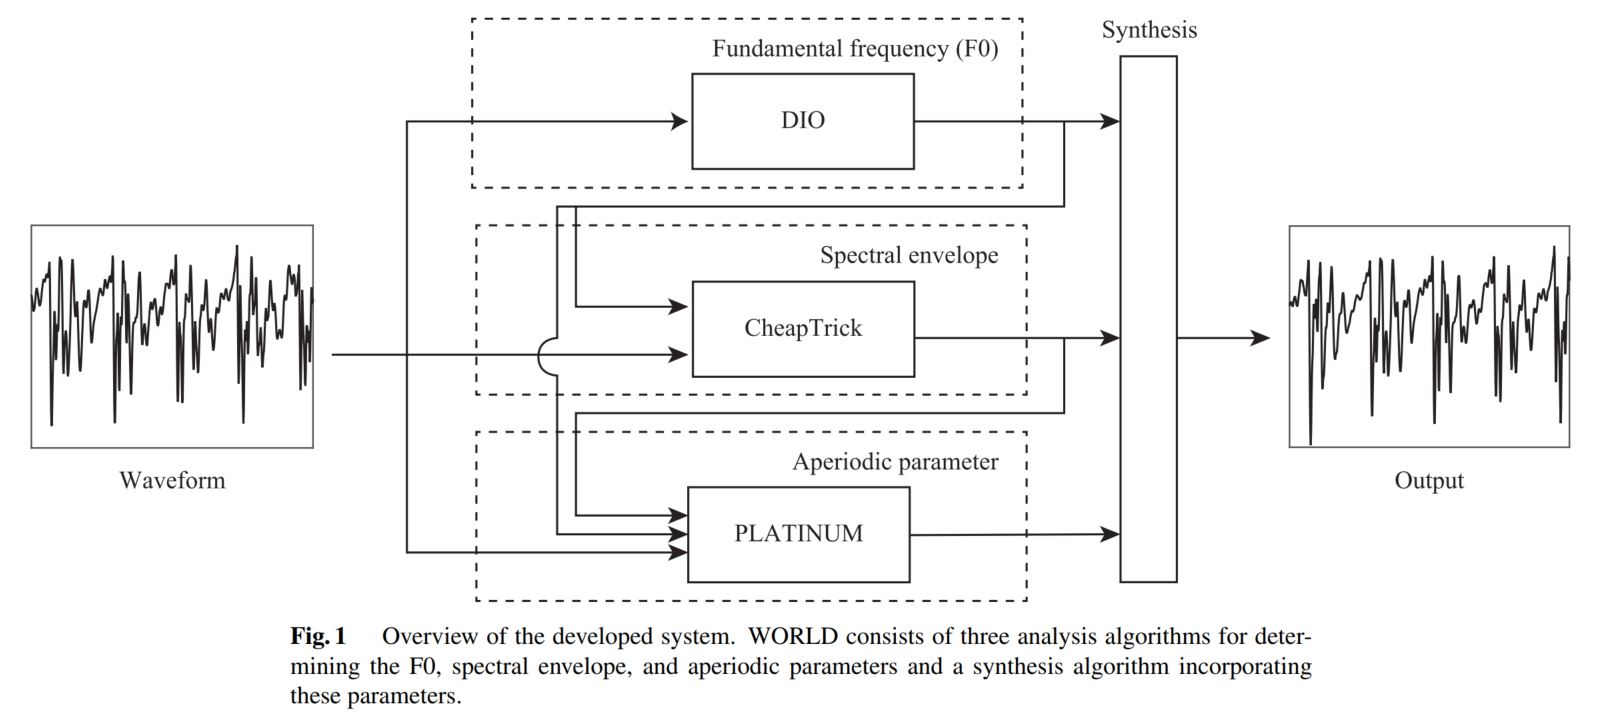
\includegraphics[width=0.6\textwidth]{vocoder_world_arch.png}
  \caption{WORLD声码器整体结构 \label{fig:vocoder_world_arch}}
\end{figure}

WORLD可以提取原始波形中的基频F0,基频包络SP和非周期信号AP,这三种声学特征对应三种提取算法:DIO输入波形提取基频,CheapTrick输入基频、波形提取频谱包络,D4C输入基频、频谱包络和波形提取非周期信号。最终,通过这三种声学特征通过最小相位谱与激励信号卷积后,输出恢复的原始波形。

\subsection{DIO算法提取基频F0}

F0是周期信号最长持续时间的倒数,反过来,周期是基频的整数分之一。基频会产生二次谐波、三次谐波等,最长的周期理论上对应着频率最低的部分,也就是在语谱图上对应最下面的亮线,能量最高的部分。

\begin{figure}[htbp]
  \centering
  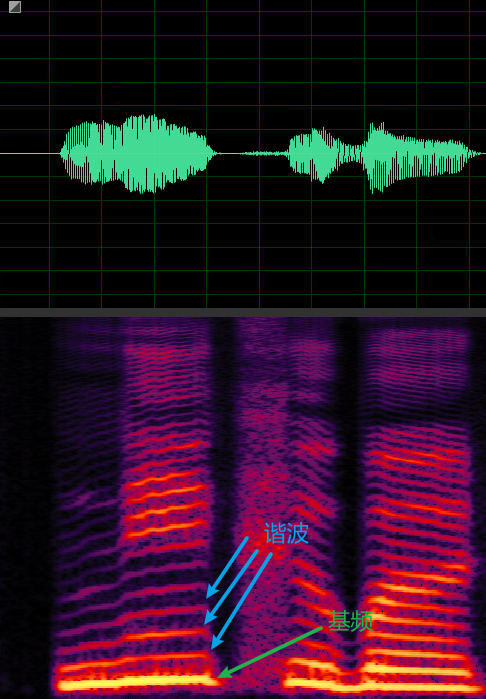
\includegraphics[width=0.6\textwidth]{vocoder_pitch_harmonic.png}
  \caption{基频和谐波 \label{fig:vocoder_pitch_harmonic}}
\end{figure}

有很多的算法估计基频F0,可以分为两类:一个是利用时域特征,比如自相关;一个利用频谱特征,比如倒谱cepstrum。WORLD使用DIO估计基频F0,比YIN、SWIPE要快,性能依然较好,DIO分为以下三步。

\begin{enumerate}
  \item 低通滤波器对原始信号进行滤波。使用不同频带的低通滤波器:因为不知道基频的位置,因此这一步包含不同周期的sin低通滤波器。
  
  \item 取4个周期计算置信度。计算获得的各个可能基频F0的置信度,因为由基频分量组成的sin信号包含4个间隔(2个顶点、2个过零点)。如果滤波器得到的间隔长度一致,则说明是一个基波,如图\ref{fig:vocoder_world_dio1}。
  
  \begin{figure}[htbp]
    \centering
    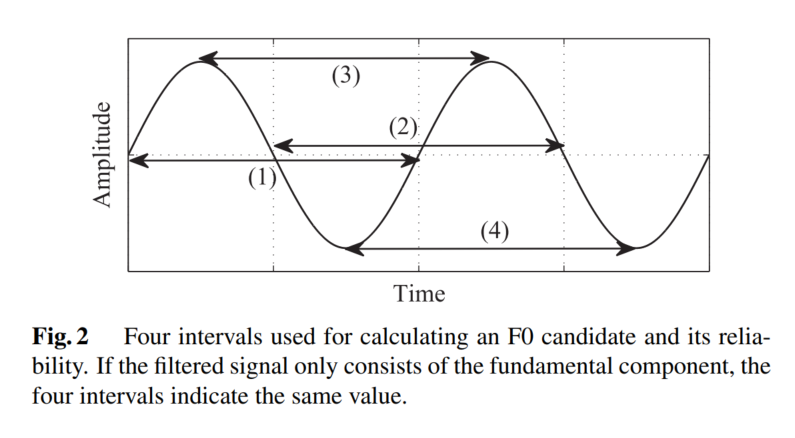
\includegraphics[width=0.6\textwidth]{vocoder_world_dio1.png}
    \caption{取四个间隔计算候选F0及其置信度 \label{fig:vocoder_world_dio1}}
  \end{figure}

  \item 从某个时间点的正弦波中提取出四个周期信号,并计算置信度,也就是标准差。然后选择标准差最低,也就是置信度最高的基波。
\end{enumerate}

\subsection{CheapTrick算法提取频谱包络SP}

声音包含不同频率的信号,覆盖0到18000Hz,每个频率都有其振幅,定义每种频率中波的振幅最高点连线形成的图形为\lstinline{包络}。频谱包络是个重要的参数,在频率-振幅图中,用平滑的曲线将所有共振峰连接起来,这个平滑的曲线就是频谱包络。

\begin{figure}[htbp]
  \centering
  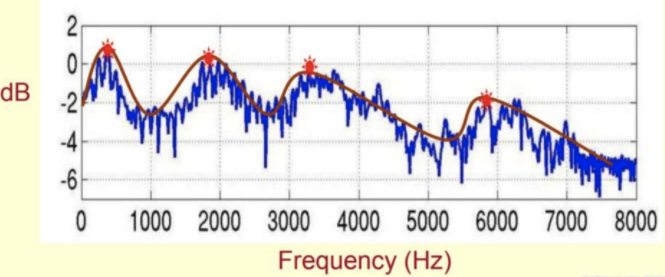
\includegraphics[width=0.6\textwidth]{vocoder_world_sp.png}
  \caption{取四个间隔计算候选F0及其置信度 \label{fig:vocoder_world_sp}}
\end{figure}

提取频谱包络SP的典型算法有线性预测编码(Linear Predictive Coding,LPC)和Cepstrum。线性预测编码LPC的原理是用若干个历史语音采样点的加权线性求和去不断逼近当前的语音采样点;Cepstrum则是基于复数倒谱拥有频谱幅度与相位信息的原理,通过对一个信号进行快速傅里叶变换FFT->取绝对值->取对数->相位展开->逆快速傅里叶变换IFFT的变换处理,从而得到对应的倒谱图。

WORLD采用CheapTrick做谱分析,思想来自于音高同步分析(pitch synchronous analysis),其过程是:先将不同基频进行自适应加窗操作,以及功率谱平滑操作,随后将信号在频域上进行同态滤波。

\subsection{PLANTINUM提取非周期信号}

混合激励和非周期信号参数AP经常应用到合成中,在Legacy-STRAIGHT和TANDEM-STRAIGHT算法中,aperiodicity被用于合成周期和非周期的信号。WORLD直接通过PLANTINUM从波形、F0和谱包络中得到混合激励的非周期信号。

\subsection{WORLD的合成算法}

TANDEM-STRAIGHT直接使用周期响应计算声带的振动,而Legacy-STRAIGHT则操纵组延迟(group delay)以避免嗡嗡声。在WORLD中,利用最小相位响应和激励信号的卷积来计算声带的振动,从下图\ref{fig:vocoder_world_synthesis},可以看到,WORLD的卷积比STAIGHT要少,因此计算量更少。

\begin{figure}[htbp]
  \centering
  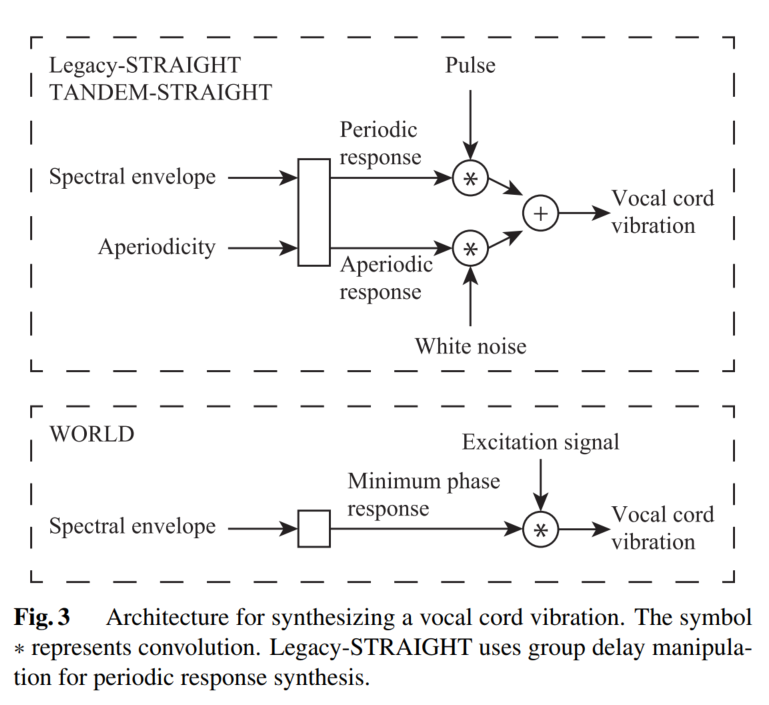
\includegraphics[width=0.6\textwidth]{vocoder_world_synthesis.png}
  \caption{WORLD合成算法 \label{fig:vocoder_world_synthesis}}
\end{figure}

\subsection{使用示例}

WORLD声码器有较为成熟的\href{https://github.com/mmorise/World}{开源实现},并且有对应的Python封装:\href{https://github.com/JeremyCCHsu/Python-Wrapper-for-World-Vocoder}{PyWORLD: A Python wrapper of WORLD Vocoder},另有\href{http://ml.cs.yamanashi.ac.jp/world/english}{官方实现}。以下示例包括了通过\lstinline{PyWorld}提取声学参数,合成原始音频,修改部分声学参数,编辑原始音频。

\begin{lstlisting}
import pyworld as pw
from scipy.io import wavfile
import matplotlib.pyplot as plt
import numpy as np
import os
import soundfile as sf

# 提取语音特征
x, fs = sf.read(WAV_FILE_PATH)

# f0 : ndarray
#     F0 contour. 基频等高线
# sp : ndarray
#     Spectral envelope. 频谱包络
# ap : ndarray
#     Aperiodicity. 非周期性
f0, sp, ap = pw.wav2world(x, fs)    # use default options

# 分别提取声学参数
# 使用DIO算法计算音频的基频F0
_f0, t = pw.dio(x, fs, f0_floor= 50.0, f0_ceil= 600.0, channels_in_octave= 2, frame_period=pw.default_frame_period)

# 使用CheapTrick算法计算音频的频谱包络
_sp = pw.cheaptrick(x, _f0, t, fs)

# 计算aperiodic参数
_ap = pw.d4c(x, _f0, t, fs)

# 基于以上参数合成原始音频
_y = pw.synthesize(_f0, _sp, _ap, fs, pw.default_frame_period)

# 1.变高频-更类似女性
high_freq = pw.synthesize(f0*2.0, sp, ap, fs)

# 2.直接修改基频,变为机器人发声
robot_like_f0 = np.ones_like(f0)*100
robot_like = pw.synthesize(robot_like_f0, sp, ap, fs)

# 3.提高基频,同时频谱包络后移 -> 更温柔的女性?
female_like_sp = np.zeros_like(sp)
for f in range(female_like_sp.shape[1]):
    female_like_sp[:, f] = sp[:, int(f/1.2)]
female_like = pw.synthesize(f0*2, female_like_sp, ap, fs)

# 4.转换基频(不能直接转换)
x2, fs2 = sf.read(WAV_FILE_PATH2)
f02, sp2, ap2 = pw.wav2world(x2, fs2)
f02 = f02[:len(f0)]
print(len(f0),len(f02))
other_like = pw.synthesize(f02, sp, ap, fs)
\end{lstlisting}

\section{Neural Homomorphic Vocoder (NHV)}

\subsection{源滤波器合成原理}

如图\ref{fig:vocoder_nhv_source_filter}所示,基于源-滤波器的参数合成中,合成器的工作流程主要可分为三步。

\begin{enumerate}
  \item 根据待合成音节的声调特性构造相应的声门波激励源。
  \item 再根据协同发音、速度变换(时长参数)等音变信息在原始声道的基础上构造出新的声道参数模型。
  \item 最后将声门波激励源送入新的声道模型中,输出就是结合给定韵律特性的合成语音。
\end{enumerate}

共振峰合成和LPC(线性预测分析)合成是上述源-滤波器结构的参数合成中最常用的两种方法,实现原理类似,只是使用的声道模型不同。同时针对声道模型的特性,在源的选取上也略有区别。

\begin{figure}[htbp]
  \centering
  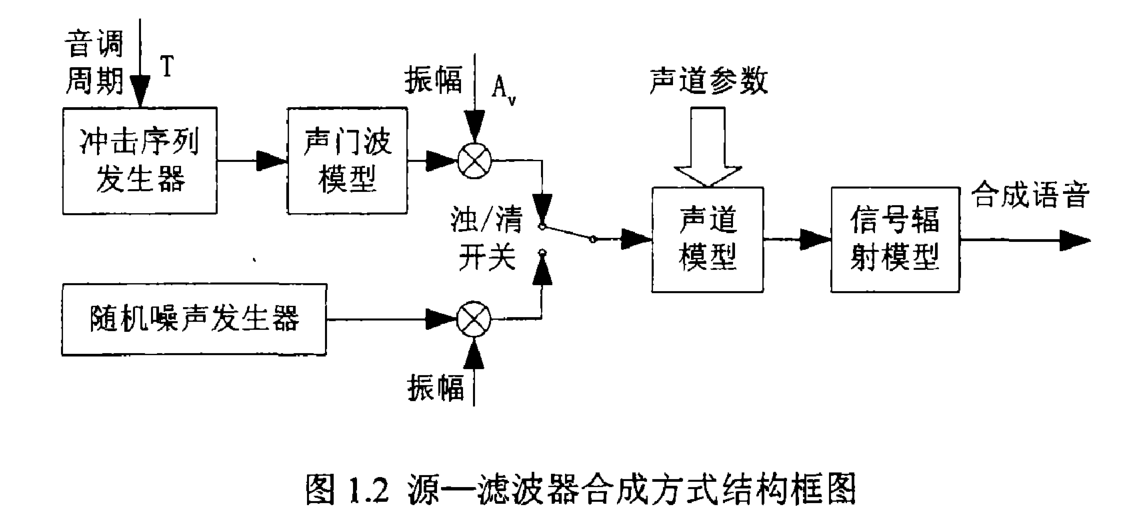
\includegraphics[width=0.6\textwidth]{vocoder_nhv_source_filter.png}
  \caption{源-滤波器合成结构框图 \label{fig:vocoder_nhv_source_filter}}
\end{figure}

\subsection{共振峰合成方法}

与线性预测方法类似,共振峰合成方法也是对声源-声道模型的模拟,但它更侧重于对声道谐振特性的模拟。它把人的声道看作一个谐振腔,腔体的谐振特性决定所发出语音信号的频谱特性,也即共振峰特性。音色各异的语音有不同的共振峰模式,用每个共振峰以及其带宽作为参数可以构成一个共振峰滤波器,将多个共振峰滤波器组合起来模拟声道的传输特性,根据这个特性对声源发生器产生的激励信号进行调制,经过辐射模型后,就可以得到合成语音。

语音学的研究结果表明,决定语音感知的声学特征主要是语音的共振峰,因此如果合成器的结构和参数设置正确,则这种方法能够合成高音质、高可懂度的语音。

\begin{enumerate}
  \item 激励源模型
  
  一般共振峰合成器的激励源有三种类型:合成浊音时用周期激励序列;合成清音时用伪随机噪音;合成浊擦音时用周期激励调制的噪音。发浊音时,声带不断地张开和关闭,产生间隙的脉冲波,开始时声门闭合幅度为零,接着声门逐渐打开,幅度缓慢上升,然后快速下降,当再次降低到零之后,有一个导数不连续点,相当于声门突然关闭。因此浊音时激励函数形式有三角波、多项式波和滤波器激励响应激励函数。

  \item 共振峰声道模型
  
  对于声道模型,声学理论表明,语音信号谱中的谐振特性(对应声道传递函数中的极点)完全由声道的形状决定,与激励源的位置无关。
\end{enumerate}

\subsection{NHV概述}

许多神经声码器旨在提升源-滤波器(source-filter)模型中对源(source)的建模能力,包括LPCNet、GELP和GlotGAN——通过神经网络仅建模源(比如建模线性预测的残差信号),而通过时变滤波器直接生成语音。不同于仅对源进行建模,神经源滤波器(Neural Source-Filter,NSF)框架将经典框架中的线性滤波器替换为卷积神经网络,其中DDSP\footnote{J. Engel, L. H. Hantrakul, C. Gu, and A. Roberts, "DDSP:
Differentiable digital signal processing," in Proc. ICLR, 2020.}通过神经网络控制谐波加性噪声(Harmonic plus Noise)生成音频。

NHV论文地址:\href{Neural Homomorphic Vocoder}{https://speechlab.sjtu.edu.cn/papers/2020/zjl00-liu-is2020.pdf}。神经同态声码器(Neural Homomorphic Vocoder,NHV)通过线性时变滤波器对脉冲串和噪音进行滤波后生成语音。给定声学特征,神经网络通过估计时变脉冲响应的复数谱控制线性时变(Linear Time-Varying,LTV)滤波器,并利用多尺度STFT和对抗损失函数进行训练。

\subsection{整体结构}

\begin{figure}[htbp]
  \centering
  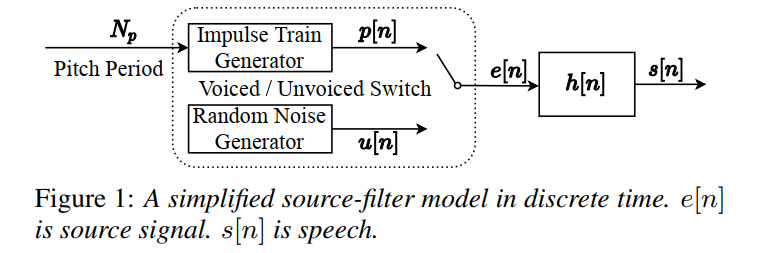
\includegraphics[width=0.6\textwidth]{vocoder_nhv_arch.png}
  \caption{源-滤波器示意图 \label{fig:vocoder_nhv_arch}}
\end{figure}

源-滤波器示意图如图\ref{fig:vocoder_nhv_arch}所示, ${e[n]}$ 表示源(source), $h[n]$ 为滤波器, $s[n]$ 则是重建的样本点。在NHV中,神经网络负责建模源-滤波器模型中的线性时变(Linear Time-Varying,LTV)滤波器。类似于谐波噪音加性模型(Harmonic plus Noise model),NHV分别生成谐波和噪音成分。谐波部分,主要是通过线性时变脉冲串(LTV filtered impulse trains)建模发音部分的周期性振动;噪音部分,包括背景噪音、不发音成分、以及发音部分中的随机成分,通过线性时变滤波噪音建模。将原始的语音信号 $x$ 和重建信号 $s$ 切分为若干个帧长 $L$ 的不重叠帧, $m$ 为帧索引, $n$ 为样本点索引, $c$ 为特征索引,因此总帧数和总样本点数满足:

\begin{equation}
  N=M\times L
\end{equation}

上式中, $N$ 表示样本点总数, $M$ 表示不重叠帧帧数,  $L$ 表示每个帧中的样本点个数。

脉冲响应 $h$ 是因果的,谐波脉冲响应 $h_h$ 和噪音脉冲响应 $h_n$ 无限长, $n\in \mathbb{Z}$ 。

\begin{figure}[htbp]
  \centering
  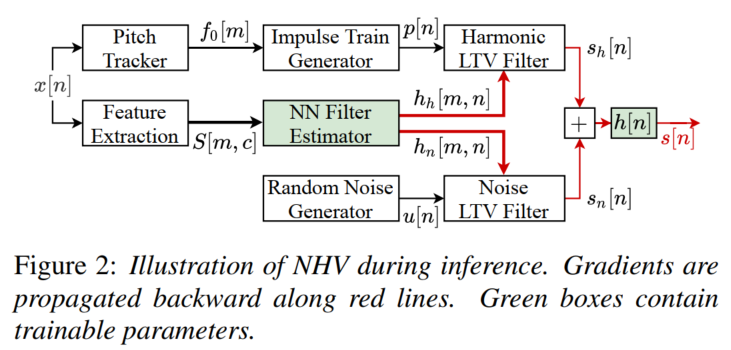
\includegraphics[width=0.6\textwidth]{vocoder_nhv_inference.png}
  \caption{NHV的语音合成过程 \label{fig:vocoder_nhv_inference}}
\end{figure}

NHV的语音生成过程如上图\ref{fig:vocoder_nhv_inference}所示,首先通过帧级别基频 $f_0[m]$ 生成脉冲串 $p[n]$ ,从高斯分布中采样得到噪音信号 $u[n]$ ;接着神经网络利用对数域梅尔谱 $S[m,c]$ 估计出每一帧的谐波脉冲响应 $h_h[m,n]$ 和噪音脉冲响应 $h_n[m,n]$ ;接着脉冲串 $p[n]$ 和噪音信号 $u[n]$ 通过LTV线性时变滤波器获得谐波成分 $s_h[n]$ 和噪音成分 $s_n[n]$ ;最后, $s_h[n]$ 和 $s_n[n]$ 加起来,并通过可训练的因果有限冲激响应滤波器 $h[n]$ 滤波,获得最终的语音样本点 $s[n]$ 。

\subsection{脉冲串生成器}

利用低通正弦波的和生成脉冲串:

\begin{equation}
  p(t)=\left\{\begin{array}{l}
    \sum_{k=1}^{2kf_0(t)<f_s}{\rm cos}(\int_{0}^{t}2\pi k f_0(\tau){\rm d}\tau),\quad if\ f_0(t)>0 \\ 
    0,\quad if\ f_0(t)=0
   \end{array}\right.
\end{equation}


其中,通过zero-order hold或者线性插值从 $f_0[m]$ 中重建 $f_0(t)$ ,且 $p[n]=p(n/f_s)$ , $f_s$ 为采样率。

由于加性生成时,根据采样率和帧移需要加和200个正弦函数,计算量较大,因此可以采用近似算法:将基频周期四舍五入到采样周期的倍数,此时离散脉冲序列是稀疏的,然后可以按顺序生成,一次生成一个音高。

\subsection{神经网络滤波估计器(Neural Network Filter Estimator)}

\begin{figure}[htbp]
  \centering
  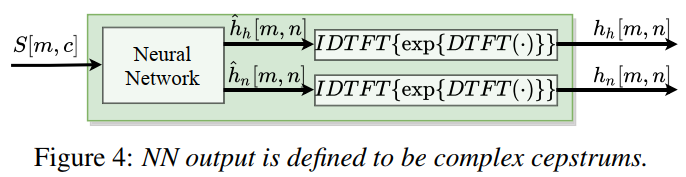
\includegraphics[width=0.6\textwidth]{vocoder_nhv_nn_filter_estimator.png}
  \caption{NHV的语音合成过程 \label{fig:vocoder_nhv_nn_filter_estimator}}
\end{figure}

使用复数谱 $\hat{h}_h$ 和 $\hat{h}_n$ 作为冲激响应 $h_h$ 和 $h_n$ 的中间表示,复数谱同时描述了幅度响应和滤波器的组延迟(group delay),滤波器的组延迟会影响语音的音色。不同于使用线性相位或最小相位滤波器,NHV使用符合相位滤波器,从数据中学习相位特性。限制复倒谱的长度相当于限制幅度和相位响应的分辨率,这提供了控制滤波器复杂性的简单方法——神经网络只预测低频带系数,高频带谱系数设置为零。实验中,每帧预测两个10ms复数谱。实现上,无限冲激响应IIR,比如 $h_h[m,n]$ 和 $h_n[m,n]$ 通过有限冲激响应FIR近似,离散傅里叶变换的窗长必须足够大,以避免混叠现象,实验中窗长设置为 $N=1024$ 。

\subsection{线性时变(LTV)滤波器和可训练的有限冲激响应(FIRs)}

FIR(有限冲激响应)常用于音频信号处理,FIR和IIR(无限冲激响应)最直观的区别就体现在结构形式上,IIR的方程中,当前的输出$y(n)$是由当前输入$x(n)$,过去输入$x(n-1),x(n-2)$和过去输出$y(n-2),y(n-1)$这三类值决定。而在FIR方程中,则没有过去输出这项。IIR的差分方程如下:

\begin{equation}
  y(n)=\sum_{k=1}^N a_ky(n-k)+\sum_{k=0}^M b_kx(n-k)
\end{equation}

而FIR的差分方程为:

\begin{equation}
  y(n)=\sum_{k=0}^M b_k x(n-k)
\end{equation}

由于IIR的当前输出受到以前输出值的影响,因此它是有反馈的,或者说输出值是递归的;而FIR就是无反馈,非递归的。

谐波部分的线性时变滤波器定义如下式所示:

\begin{equation}
  s_h[n]=\sum_{m=0}^{M}(w_L[n-mL]\cdot p[n])*h_h[m,n]
\end{equation}

卷积可以在时域和频域上应用,可训练的FIR滤波器 $h[n]$ 可以应用到语音生成的最后一步,谐波部分的卷积过程如下图所示。

\begin{figure}[htbp]
  \centering
  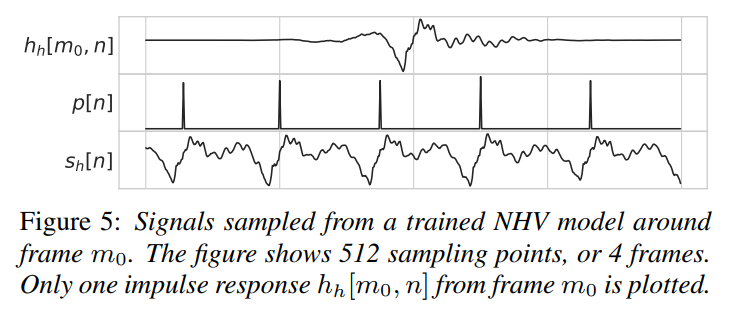
\includegraphics[width=0.6\textwidth]{vocoder_nhv_harmonic_sample.png}
  \caption{谐波部分的卷积过程 \label{fig:vocoder_nhv_harmonic_sample}}
\end{figure}

\subsection{神经网络的训练}

\begin{enumerate}
  \item 多尺度STFT损失
  
  因为要求原始信号 $x$ 和重建信号 $s$ 的声门激励(Glottal Closure Instants,GCIs)完全对齐,因此在重建信号 $x[n]$ 和原始信号 $s[n]$ 之间无法施加点级损失,而多尺度STFT计算损失时允许信号间相位错位。类似于多子带MelGAN\footnote{Yang G, Yang S, Liu K, et al. Multi-band MelGAN: Faster waveform generation for high-quality text-to-speech[C]. 2021 IEEE Spoken Language Technology Workshop (SLT). IEEE, 2021: 492-498.},多尺度STFT损失定义为不同参数下原始和重建幅度谱之间的L1距离之和:

  \begin{equation}
    {\rm L}_R=\frac{1}{C}\sum_{i=0}^{C-1}\frac{1}{K_i}(||X_i-S_i||_1+||{\rm log}X_i-{\rm log}S_i||_1)
  \end{equation}

  上式中, $X_i$ 和 $S_i$ 分别为原始信号 $x$ 和重建信号 $s$ 在参数 $i$ 设置下计算获得的幅度谱,每个幅度谱包括 $K_i$ 个值,共 $C$ 组STFT参数配置,组数越多,重建信号的混叠问题一般越少。

  \item 对抗损失函数
  
  NHV采取合页损失函数形式:

  \begin{equation}
    {\rm L}_D=\mathbb{E}_{x,S}[{\rm max}(0,1-D(x,S))]+\mathbb{E}_{f_0,S}[{\rm max}(0,1+D(G(f_0,S),S))]
  \end{equation}
  \begin{equation}
    {\rm G}=\mathbb{E}_{f_0,S}[-D(G(f_0,S),S)]
  \end{equation}

  上式中, $D(x,S)$ 表示判别器网络, $D$ 输入原始信号 $x$ 或重建信号 $s$ ,以及真实log域梅尔频谱 $S$ , $f_0$ 表示基频,生成器 $G(f_0,S)$ 输出重建信号 $s$ 。
\end{enumerate}

\subsection{小结}

NHV是基于源-滤波器的神经声码器,通过神经网络建模线性时变滤波器(LTV),对脉冲串和噪音进行滤波后生成语音,并结合多尺度STFT和对抗损失进行训练。

\section{HiFiGAN}

\subsection{HiFiGAN概述}

HiFiGAN是近年来在学术界和工业界都较为常用的声码器,能够将声学模型产生的频谱转换为高质量的音频,这种声码器采用生成对抗网络(Generative Adversial Networks,GAN)作为基础生成模型,相比于之前相近的MelGAN,改进点在于:

\begin{enumerate}
  \item 引入了多周期判别器(Multi-Period Discriminator,MPD)。HiFiGAN同时拥有多尺度判别器(Multi-Scale Discriminator,MSD)和多周期判别器,尽可能增强GAN判别器甄别合成或真实音频的能力,从而提升合成音质。
  \item 生成器中提出了多感受野融合模块。WaveNet为了增大感受野,叠加带洞卷积,音质虽然很好,但是也使得模型较大,推理速度较慢。HiFiGAN则提出了一种残差结构,交替使用带洞卷积和普通卷积增大感受野,保证合成音质的同时,提高推理速度。
\end{enumerate}

\subsection{HiFiGAN生成器简介}

HiFiGAN的生成器主要有两块,一个是上采样结构,具体由一维转置卷积组成;二是所谓的多感受野融合(Multi-Receptive Field Fusion,MRF)模块,主要负责对上采样获得的采样点进行优化,具体由残差网络组成。

\subsection{上采样结构}

作为声码器的生成器,不但需要负责将频谱从频域转换到时域,而且要进行上采样(upsampling)。以80维梅尔频谱合成16kHz的语音为例,假设帧移为10ms,则每个帧移内有160个语音样本点,需要通过80个梅尔频谱值获得,因此,需要利用卷积网络不断增加输出“长度”,降低输出“通道数”,直到上采样倍数达到160,通道数降低为1即可。

对于上采样操作,可以使用插值算法进行处理,比如最近邻插值(Nearest neighbor interpolation)、双线性插值(Bi-Linear interpolation)、双立方插值(Bi-Cubic interpolation)等,但是这些插值算法说到底是人工规则,而神经网络可以自动学习合适的变换,\href{https://pytorch.org/docs/master/generated/torch.nn.ConvTranspose1d.html}{转置卷积(ConvTransposed)},也称反卷积Deconvolution、微步卷积Fractionally-strided Convolution,则是合适的上采样结构。一般的卷积中,每次卷积操作都是对输入张量和卷积核的每个元素进行相乘再加和,卷积的输入和输出是\lstinline{多对一}的映射关系,而转置卷积则反过来,是\lstinline{一对多}的映射关系。从计算机的内部实现来看,定义:

\begin{enumerate}
  \item $X$ 为输入张量,大小为 $X_{width}\times X_{height}$ 
  \item $Y$ 为输出张量,大小为 $Y_{width}\times Y_{height}$ 
  \item $C$ 为卷积核,大小为 $C_{width}\times C_{height}$ 
\end{enumerate}

经过普通的卷积运算之后,将大张量 $X$ “下采样”到小张量 $Y$ 。具体来说,首先将输入张量展平为向量,也即是 $[X_{width}\times X_{height},1]$ ,同时也将卷积核展平成向量到输入张量 $X$ 的大小:由于卷积核小于输入张量,在行和列上都用0填充至输入张量大小,然后展平,则卷积核向量大小为 $[1,X_{width}\times X_{height}]$ ;同时按照步长,左侧填充0偏移该卷积核向量,最终,卷积核向量的个数为输出张量元素个数,则构成的卷积核张量大小为 $[Y_{width}\times Y_{height},X_{width}\times X_{height}]$ ,卷积核张量和输入张量矩阵乘,获得输出张量 $[Y_{width}\times Y_{height},1]$ ,重塑大小为 $C_{width},C_{height}$ 。

此时,如果使用卷积核张量的转置 $[X_{width}\times X_{height},Y_{width}\times Y_{height}]$ 矩阵乘展平的 $[Y_{width}\times Y_{height},1]$ ,得到的结果就是 $[X_{width}\times X_{height},1]$ ,和刚刚的输入张量大小相同,这就完成了一次\lstinline{转置卷积}。但实际上,上述操作并非可逆关系,卷积将输入张量“下采样”到输出张量,本质是有损压缩的过程,由于在卷积中使用的\lstinline{卷积核张量}并非可逆矩阵,转置卷积操作之后并不能恢复到原始的数值,仅仅是恢复到原始的形状。这其实也就是线性谱与梅尔频谱关系,加权求和得到梅尔频谱之后就回不来了,顶多求梅尔滤波器组的伪逆,近似恢复到线性谱。

此外,在使用转置卷积时需要注意棋盘效应(Checkboard artifacts)。棋盘效应主要是由于转置卷积的“不均匀重叠”(Uneven overlap)造成的,输出中每个像素接受的信息量与相邻像素不同,在输出上找不到连续且均匀重叠的区域,表现是图像中一些色块的颜色比周围色块要深,像棋盘上的方格,参见\href{https://distill.pub/2016/deconv-checkerboard}{Deconvolution and Checkerboard Artifacts}。避免棋盘效应的方法主要有:kernel\_size的大小尽可能被stride整除,尽可能使用stride=1的转置卷积;堆叠转置卷积减轻重叠;网络末尾使用 $1\times 1$ 的转置卷积等。

通过上述的原理部分,可以看出卷积和转置卷积是对偶运算,输入变输出,输出变输入,卷积的输入输出大小关系为:

\begin{equation}
  L_{out}=\frac{L_{in}+2\times padding-kernel\_size}{stride}+1
\end{equation}

那么转置卷积的输入输出大小则为:

\begin{equation}
  L_{out}=(L_{in}-1)\times stride+kernel\_size-2\times padding
\end{equation}

当然,加入dilation之后,大小计算稍复杂些,参见\href{https://pytorch.org/docs/master/generated/torch.nn.ConvTranspose1d.html}{Pytorch-ConvTranspose1d},\href{https://pytorch.org/docs/master/generated/torch.nn.Conv1d.html}{Pytorch-Conv1d}。

该部分参考文献:

\begin{enumerate}
  \item \href{https://www.zhihu.com/question/48279880/answer/1682194600}{怎样通俗易懂地解释反卷积?}
  \item \href{https://zhuanlan.zhihu.com/p/158933003}{一文搞懂反卷积,转置卷积}
  \item \href{https://distill.pub/2016/deconv-checkerboard}{Deconvolution and Checkerboard Artifacts}
  \item \href{https://www.zhihu.com/question/436832427/answer/1679396968}{如何去除生成图片产生的棋盘伪影?}
  \item \href{https://arxiv.org/abs/1603.07285}{A guide to convolution arithmetic for deep learning}
  \item \href{https://pytorch.org/docs/master/generated/torch.nn.ConvTranspose1d.html}{Pytorch-ConvTranspose1d}
  \item \href{https://pytorch.org/docs/master/generated/torch.nn.Conv1d.html}{Pytorch-Conv1d}
\end{enumerate}
  
转置卷积实现的上采样层定义为:

\begin{lstlisting}
self.ups = nn.ModuleList()
for i, (u, k) in enumerate(zip(h.upsample_rates, h.upsample_kernel_sizes)):
    self.ups.append(weight_norm(ConvTranspose1d(h.upsample_initial_channel//(2**i), 
    h.upsample_initial_channel//(2**(i+1)),kernel_size=k, 
    stride=u, padding=(k-u)//2)))
\end{lstlisting}

对于hop\_size=256来说,h.upsample\_rates和h.upsample\_kernel\_sizes分别为:

\begin{enumerate}
  \item "upsample\_rates": [8,8,2,2],
  \item "upsample\_kernel\_sizes": [16,16,4,4],
\end{enumerate}

根据转置卷积的输入输出大小关系:

\begin{equation}
  L_{out}=(L_{in}-1)\times stride-2\times padding+dilation\times (kernel\_size-1)+output\_padding+1
\end{equation}

用于上采样的转置卷积,通过设置合适的padding,配合卷积核大小(kernel\_size)和步进(stride),就可以实现输出与输入大小呈“步进倍数”的关系,在这里,卷积核(upsample\_kernel\_sizes)设置为步进(upsample\_rates)的2倍。设置参数时,必须保持帧移点数,是各个卷积层步进(或者代码中所谓的上采样率update\_rates)的乘积,在上例中,也就是:

\begin{equation}
  hop\_length=256=8\times 8\times 2\times 2
\end{equation}

\subsection{多感受野融合}

转置卷积的上采样容易导致棋盘效应,因此每次转置卷积上采样之后,都会跟着一个多感受野融合(MRF)的残差网络,以进一步提升样本点的生成质量。多感受野融合模块是一种利用带洞卷积和普通卷积提高生成器感受野的结构,带洞卷积的扩张倍数逐步递增,如dilation=1,3,5,每个带洞卷积之后,跟着卷积核大于1的普通卷积,从而实现带洞卷积和普通卷积的交替使用。带洞卷积和普通卷积的输入输出大小保持不变,在一轮带洞和普通卷积完成之后,原始输入跳连到卷积的结果,从而实现一轮“多感受野融合”。多感受野融合的具体实现上,论文中提出了两种参数量不同的残差网络。一种是参数量较多,多组带洞卷积(dilation=1,3,5)和普通卷积交替使用,HiFiGAN v1 (config\_v1.json)和HiFiGAN v2 (config\_v2.json)均使用该种多感受野融合(MRF)模块。:

\begin{lstlisting}
class ResBlock1(torch.nn.Module):
    def __init__(self, h, channels, kernel_size=3, dilation=(1, 3, 5)):
        super(ResBlock1, self).__init__()
        self.h = h
        self.convs1 = nn.ModuleList([
            weight_norm(Conv1d(channels, channels, kernel_size, 1, 
              dilation=dilation[0],padding=get_padding(kernel_size, dilation[0]))),
            weight_norm(Conv1d(channels, channels, kernel_size, 1, 
              dilation=dilation[1], padding=get_padding(kernel_size, dilation[1]))),
            weight_norm(Conv1d(channels, channels, kernel_size, 1, 
              dilation=dilation[2], padding=get_padding(kernel_size, dilation[2]))),
        ])
        self.convs1.apply(init_weights)

        self.convs2 = nn.ModuleList([
            weight_norm(Conv1d(channels, channels, kernel_size, 1, dilation=1,
                                padding=get_padding(kernel_size, 1))),
            weight_norm(Conv1d(channels, channels, kernel_size, 1, dilation=1,
                                padding=get_padding(kernel_size, 1))),
            weight_norm(Conv1d(channels, channels, kernel_size, 1, dilation=1,
                                padding=get_padding(kernel_size, 1)))
        ])
        self.convs2.apply(init_weights)

    def forward(self, x):
        for c1, c2 in zip(self.convs1, self.convs2):
            xt = F.leaky_relu(x, LRELU_SLOPE)
            xt = c1(xt)
            xt = F.leaky_relu(xt, LRELU_SLOPE)
            xt = c2(xt)
            x = xt + x
        return x

    def remove_weight_norm(self):
        for l in self.convs1:
            remove_weight_norm(l)
        for l in self.convs2:
            remove_weight_norm(l)
\end{lstlisting}

另外一种MRF大大减少了参数量,仅由两层带洞卷积(dilation=1,3)组成,但依然保持了跳跃连接的结构:

\begin{lstlisting}
class ResBlock2(torch.nn.Module):
    def __init__(self, h, channels, kernel_size=3, dilation=(1, 3)):
        super(ResBlock2, self).__init__()
        self.h = h
        self.convs = nn.ModuleList([
            weight_norm(Conv1d(channels, channels, kernel_size, 1, 
              dilation=dilation[0], padding=get_padding(kernel_size, dilation[0]))),
            weight_norm(Conv1d(channels, channels, kernel_size, 1, 
              dilation=dilation[1], padding=get_padding(kernel_size, dilation[1]))),
        ])
        self.convs.apply(init_weights)

    def forward(self, x):
        for c in self.convs:
            xt = F.leaky_relu(x, LRELU_SLOPE)
            xt = c(xt)
            x = xt + x
        return x

    def remove_weight_norm(self):
        for l in self.convs:
            remove_weight_norm(l)
\end{lstlisting}

注意到两种MRF都使用了weight\_norm对神经网络的权重进行规范化,相比于batch\_norm,weight\_norm不依赖mini-batch的数据,对噪音数据更为鲁棒;并且,可以应用于RNN等时序网络上;此外,weight\_norm直接对神经网络的权重值进行规范化,前向和后向计算时,带来的额外计算和存储开销都较小。weight\_norm本质是利用方向 $v$ 和幅度张量 $g$ 替代权重张量 $w$ :

\begin{equation}
  w=g\frac{v}{||v||}
\end{equation}

方向张量 $v$ 和 $w$ 大小相同,幅度张量 $g$ 比 $w$ 少一维,使得 $w$ 能够比较容易地整体缩放。不直接优化 $w$ ,而是训练 $v$ 和 $g$ 。

同时注意到,在推理时需要remove\_weight\_norm,这是因为训练时需要计算权重矩阵的方向和幅度张量,而在推理时,参数已经优化完成,要恢复回去,所以在推理时就直接移除weight\_norm机制。

每个卷积核的0填充个数都调用了get\_padding函数,利用填充保证输入输出的长宽大小一致,该填充大小的计算方法:

\begin{equation}
  padding=(kernel\_size-1)*padding//2
\end{equation}

\subsection{HiFiGAN判别器简介}

HiFiGAN的判别器有两个,分别是多尺度和多周期判别器,从两个不同角度分别鉴定语音。多尺度判别器源自MelGAN声码器的做法,不断平均池化语音序列,逐次将语音序列的长度减半,然后在语音的不同尺度上施加若干层卷积,最后展平,作为多尺度判别器的输出。多周期判别器则是以不同的序列长度将一维的音频序列折叠为二维平面,在二维平面上施加二维卷积。

\subsection{多尺度判别器}

多尺度判别器的核心是多次平均池化,缩短序列长度,每次序列长度池化至原来的一半,然后进行卷积。具体来说,多尺度判别器首先对原样本点进行一次“原尺寸判别”,其中“原尺寸判别”模块中一维卷积的参数规范化方法为谱归一化(spectral\_norm);接着对样本点序列进行平均池化,依次将序列长度减半,然后对“下采样”的样本点序列进行判别,该模块中一维卷积的参数规范化方法为权重归一化(weight\_norm)。在每一个特定尺度的子判别器中,首先进行若干层分组卷积,并对卷积的参数进行规范化;接着利用leaky\_relu进行激活;在经过多个卷积层之后,最后利用输出通道为1的卷积层进行后处理,展平后作为输出。

\begin{lstlisting}
class MultiScaleDiscriminator(torch.nn.Module):
    def __init__(self):
        super(MultiScaleDiscriminator, self).__init__()
        self.discriminators = nn.ModuleList([
            DiscriminatorS(use_spectral_norm=True),
            DiscriminatorS(),
            DiscriminatorS(),
        ])
        self.meanpools = nn.ModuleList([
            AvgPool1d(4, 2, padding=2),
            AvgPool1d(4, 2, padding=2)
        ])

    def forward(self, y, y_hat):
        y_d_rs = []
        y_d_gs = []
        fmap_rs = []
        fmap_gs = []
        for i, d in enumerate(self.discriminators):
            if i != 0:
                y = self.meanpools[i-1](y)
                y_hat = self.meanpools[i-1](y_hat)
            y_d_r, fmap_r = d(y)
            y_d_g, fmap_g = d(y_hat)
            y_d_rs.append(y_d_r)
            fmap_rs.append(fmap_r)
            y_d_gs.append(y_d_g)
            fmap_gs.append(fmap_g)

        return y_d_rs, y_d_gs, fmap_rs, fmap_gs
\end{lstlisting}

上述代码中y\_d\_rs和y\_d\_gs分别是真实和生成样本的多尺度判别器展平后的整体输出,fmap\_rs和y\_d\_gs分别是真实和生成样本经过每一层卷积的特征图(feature map)。子判别器DiscriminatorS由若干层卷积组成,最后一层输出通道为1,之后对输出进行展平。注意到,与MelGAN不同,多尺度判别器的第一个子判别器DiscriminatorS使用谱归一化spectral\_norm,之后两个子判别器则是正常使用权重归一化weight\_norm规整可训练参数。谱归一化实际是在每次更新完可训练参数 $W$ 之后,都除以 $W$ 的奇异值,以保证整个网络满足利普希茨连续性,使得GAN的训练更稳定。参见\href{https://kaizhao.net/posts/spectral-norm}{GAN 的谱归一化(Spectral Norm)和矩阵的奇异值分解(Singular Value Decompostion)}。DiscriminatorS的具体实现如下:

\begin{lstlisting}
class DiscriminatorS(torch.nn.Module):
    def __init__(self, use_spectral_norm=False):
        super(DiscriminatorS, self).__init__()
        norm_f = weight_norm if use_spectral_norm == False else spectral_norm
        self.convs = nn.ModuleList([
            norm_f(Conv1d(1, 128, 15, 1, padding=7)),
            norm_f(Conv1d(128, 128, 41, 2, groups=4, padding=20)),
            norm_f(Conv1d(128, 256, 41, 2, groups=16, padding=20)),
            norm_f(Conv1d(256, 512, 41, 4, groups=16, padding=20)),
            norm_f(Conv1d(512, 1024, 41, 4, groups=16, padding=20)),
            norm_f(Conv1d(1024, 1024, 41, 1, groups=16, padding=20)),
            norm_f(Conv1d(1024, 1024, 5, 1, padding=2)),
        ])
        self.conv_post = norm_f(Conv1d(1024, 1, 3, 1, padding=1))

    def forward(self, x):
        fmap = []
        for l in self.convs:
            x = l(x)
            x = F.leaky_relu(x, LRELU_SLOPE)
            fmap.append(x)
        x = self.conv_post(x)
        fmap.append(x)
        x = torch.flatten(x, 1, -1)

        return x, fmap
\end{lstlisting}

x是子判别器展平后的整体输出,大小为[B,l];fmap是经过卷积后的特征图(feature map),类型为list,元素个数为卷积层数,上述代码中有8个卷积层,则fmap元素个数为8,每个元素均是大小为[B,C,l']的张量。

\subsection{多周期判别器}

多周期判别器的重点是将一维样本点序列以一定周期折叠为二维平面,例如一维样本点序列[1,2,3,4,5,6],如果以3为周期,折叠成二维平面则是[[1,2,3],[4,5,6]],然后对这个二维平面施加二维卷积。具体来说,每个特定周期的子判别器首先进行填充,保证样本点数是周期的整倍数,以方便“折叠”为二维平面;接下来进入多个卷积层,输出通道数分别为[32,128,512,1024],卷积之后利用leaky\_relu激活,卷积层参数规范化方法均为权重归一化(weight\_norm);然后经过多个卷积层之后,利用一个输入通道数为1024,输出通道为1的卷积层进行后处理;最后展平,作为多周期判别器的最终输出。多周期判别器包含多个周期不同的子判别器,在论文代码中周期数分别设置为[2,3,5,7,11]。

\begin{lstlisting}
class MultiPeriodDiscriminator(torch.nn.Module):
    def __init__(self):
        super(MultiPeriodDiscriminator, self).__init__()
        self.discriminators = nn.ModuleList([
            DiscriminatorP(2),
            DiscriminatorP(3),
            DiscriminatorP(5),
            DiscriminatorP(7),
            DiscriminatorP(11),
        ])

    def forward(self, y, y_hat):
        y_d_rs = []
        y_d_gs = []
        fmap_rs = []
        fmap_gs = []
        for i, d in enumerate(self.discriminators):
            y_d_r, fmap_r = d(y)
            y_d_g, fmap_g = d(y_hat)
            y_d_rs.append(y_d_r)
            fmap_rs.append(fmap_r)
            y_d_gs.append(y_d_g)
            fmap_gs.append(fmap_g)

        return y_d_rs, y_d_gs, fmap_rs, fmap_gs
\end{lstlisting}

上述代码中y\_d\_rs和y\_d\_gs分别是真实和生成样本的多周期判别器输出,fmap\_rs和fmap\_gs分别是真实和生成样本经过每一层卷积后输出的特征图(feature map)。子判别器DiscriminatorP由若干层二维卷积组成:

\begin{lstlisting}
class DiscriminatorP(torch.nn.Module):
    def __init__(self, period, kernel_size=5, stride=3, use_spectral_norm=False):
        super(DiscriminatorP, self).__init__()
        self.period = period
        norm_f = weight_norm if use_spectral_norm == False else spectral_norm
        self.convs = nn.ModuleList([
            norm_f(Conv2d(1, 32, (kernel_size, 1), (stride, 1), padding=(get_padding(5, 1), 0))),
            norm_f(Conv2d(32, 128, (kernel_size, 1), (stride, 1), padding=(get_padding(5, 1), 0))),
            norm_f(Conv2d(128, 512, (kernel_size, 1), (stride, 1), padding=(get_padding(5, 1), 0))),
            norm_f(Conv2d(512, 1024, (kernel_size, 1), (stride, 1), padding=(get_padding(5, 1), 0))),
            norm_f(Conv2d(1024, 1024, (kernel_size, 1), 1, padding=(2, 0))),
        ])
        self.conv_post = norm_f(Conv2d(1024, 1, (3, 1), 1, padding=(1, 0)))

    def forward(self, x):
        fmap = []

        # 1d to 2d
        b, c, t = x.shape
        if t % self.period != 0: # pad first
            n_pad = self.period - (t % self.period)
            x = F.pad(x, (0, n_pad), "reflect")
            t = t + n_pad
        x = x.view(b, c, t // self.period, self.period)

        for l in self.convs:
            x = l(x)
            x = F.leaky_relu(x, LRELU_SLOPE)
            fmap.append(x)
        x = self.conv_post(x)
        fmap.append(x)
        x = torch.flatten(x, 1, -1)

        return x, fmap
\end{lstlisting}

x是子判别器展平后的整体输出,大小为[B,l];fmap是经过每一层卷积后的特征图(feature map),类型为list,元素个数为卷积层数,上述代码中有6个卷积层,则fmap元素个数为6,每个元素是大小为[B,C,l',period]的张量。

\subsection{损失函数简介}

HiFiGAN的损失函数主要包括三块,一个是GAN原始的生成对抗损失(GAN Loss);第二是梅尔频谱损失(Mel-Spectrogram Loss),将生成音频转换回梅尔频谱之后,计算真实和生成音频对应梅尔频谱之间的L1距离;第三是特征匹配损失(Feature Match Loss),主要是对比真实和合成音频在中间卷积层上的差异。

\subsection{生成对抗损失}

HiFiGAN仍然是一个生成对抗网络,判别器计算输入是真实样本的概率,生成器生成以假乱真的样本,最终达到生成器合成接近真实的样本,以致于判别器无法区分真实和生成样本。HiFiGAN使用\href{https://zhuanlan.zhihu.com/p/25768099}{最小二乘GAN(LS-GAN)},将原始GAN中的二元交叉熵替换为最小二乘损失函数。判别器的生成对抗损失定义为:

\begin{equation}
  {\rm L}_{Adv}(D;G)=\mathbb{E}_{(x,s)}[(D(x)-1)^2+(D(G(s)))^2]
\end{equation}

对应的代码实现:

\begin{lstlisting}
def discriminator_loss(disc_real_outputs, disc_generated_outputs):
    loss = 0
    r_losses = []
    g_losses = []
    for dr, dg in zip(disc_real_outputs, disc_generated_outputs):
        r_loss = torch.mean((dr-1)**2)
        g_loss = torch.mean(dg**2)
        loss += (r_loss + g_loss)
        r_losses.append(r_loss.item())
        g_losses.append(g_loss.item())

    return loss, r_losses, g_losses
\end{lstlisting}

生成器的生成对抗损失定义为:

\begin{equation}
  
\end{equation}


















\section{ElegantBook 更新说明}

此次为 4.x 第一个版本,在 3.x 基础上,主要更新了定理以及参考文献的支持方式,具体内容有:

\begin{enumerate}
  \item \textbf{重要改动}:由原先的 \hologo{BibTeX} 改为 biblatex 编译方式(后端为 \lstinline{biber}),请注意两者之间的差异;
  \item \textbf{重要改进}:修改对于定理写法兼容方式,提高数学公式代码的兼容性;
  \item 页面设置改动,默认页面更宽;方便书写和阅读;
  \item 支持目录文字以及页码跳转;
  \item 不再维护 \hologo{pdfLaTeX} 中文支持方式,请务必使用 \hologo{XeLaTeX} 编译中文文稿。
  \item 增加多语言选项,法语 \lstinline{lang=fr}、德语 \lstinline{lang=de}、荷兰语 \lstinline{lang=nl}、匈牙利语 \lstinline{lang=hu}、西班牙语 \lstinline{lang=es}、蒙古语 \lstinline{lang=mn} 等。
\end{enumerate}

\begin{note}
如果你使用旧版本切换到新版本时,遇到问题时,请核对文档中是否有 \lstinline{pageanchor} 字样。如果有,请删除文档中的 \lstinline|\hypersetup{pageanchor=true}|,并且在 \lstinline{\maketitle} 和 \lstinline{\tableofcontents} 之间添加 \lstinline{\frontmatter}。2.x 版本的用户请仔细查看\href{https://github.com/ElegantLaTeX/ElegantBook/wiki/convert}{跨版本转换}。
\end{note}

\section{模板安装与更新}

你可以通过免安装的方式使用本模板,包括在线使用和本地(文件夹内)使用两种方式,也可以通过 \TeX{} 发行版安装使用。

\subsection{在线使用模板}

我们把三套模板全部上传到 \href{https://www.overleaf.com/}{Overleaf} 上了,网络便利的用户可以直接通过 Overleaf 在线使用我们的模板。使用 Overleaf 的好处是无需安装 \TeX{} Live 2020,可以随时随地访问自己的文件。查找模板,请在 Overleaf 模板库里面搜索 \lstinline{elegantlatex} 即可,你也可以直接访问\href{https://www.overleaf.com/latex/templates?addsearch=elegantlatex}{搜索结果}。选择适当的模板之后,将其 \lstinline{Open as Template},即可把模板存到自己账户下,然后可以自由编辑以及与别人一起协作。更多关于 Overleaf 的介绍和使用,请参考 Overleaf 的\href{https://www.overleaf.com/learn}{官方文档}。

\begin{remark}
Overleaf 上,中文需要使用 \hologo{XeLaTeX} 进行编译,英文建议使用 \hologo{pdfLaTeX} 编译。
\end{remark}

\subsection{本地免安装使用}

\textbf{免安装}使用方法如下,从 GitHub 或者 CTAN 下载最新版,严格意义上只需要类文件 \lstinline{elegantbook.cls}。然后将模板文件放在你的工作目录下即可使用。这样使用的好处是,无需安装,简便;缺点是,当模板更新之后,你需要手动替换 \lstinline{cls} 文件。

\subsection{发行版安装使用}

本模板测试环境为 Win10 和 TeX Live 2021,如果你刚安装 \TeX{} Live 2021 用户,安装后建议升级全部宏包,升级方法:使用 cmd 运行 \lstinline{tlmgr update --all},如果 tlmgr 需要更新,请使用 cmd 运行 \lstinline{tlmgr update --self},如果更新过程中出现了中断,请改用 \lstinline{tlmgr update --self --all --reinstall-forcibly-removed} 更新。

\subsection{更新问题}

如果使用 \lstinline{tlshell} 无法更新模板,请使用命令行全部更新全部宏包或者使用免安装的方法使用本模板。

通过命令行(管理员权限)输入下面的命令对 tlmgr 自身和全部宏包进行更新。

\begin{lstlisting}
  tlmgr update --self 
  tlmgr update --all
\end{lstlisting}

更多的内容请参考 \href{https://tex.stackexchange.com/questions/55437/how-do-i-update-my-tex-distribution}{How do I update my \TeX{} distribution?}

\subsection{其他发行版本}

由于宏包版本问题,本模板不支持 C\TeX{} 套装,请务必安装 TeX Live。更多关于 \TeX{} Live 的安装使用以及 C\TeX{} 与 \TeX{} Live 的兼容、系统路径问题,请参考官方文档以及啸行的\href{https://github.com/OsbertWang/install_latex/releases}{一份简短的安装 \LaTeX{} 的介绍}。


\section{关于提交}

出于某些因素的考虑,Elegant\LaTeX{} 项目自 2019 年 5 月 20 日开始,\textbf{不再接受任何非作者预约性质的提交}(pull request)!如果你想改进模板,你可以给我们提交 issues,或者可以在遵循协议(LPPL-1.3c)的情况下,克隆到自己仓库下进行修改。


\chapter{ElegantBook 设置说明}

本模板基于基础的 book 文类,所以 book 的选项对于本模板也是有效的(纸张无效,因为模板有设备选项)。默认编码为 UTF-8,推荐使用 \TeX{} Live 编译。本文编写环境为 Win10 (64bit) + \TeX{} Live 2021,英文支持 \hologo{pdfLaTeX},中文仅支持 \hologo{XeLaTeX} 编译。

\section{语言模式}
本模板内含两套基础语言环境 \lstinline{lang=cn}、\lstinline{lang=en}。改变语言环境会改变图表标题的引导词(图,表),文章结构词(比如目录,参考文献等),以及定理环境中的引导词(比如定理,引理等)。不同语言模式的启用如下:
\begin{lstlisting}
\documentclass[cn]{elegantbook} 
\documentclass[lang=cn]{elegantbook}
\end{lstlisting}

除模板自带的两套语言设定之外,由网友提供的其他语言环境设置如下:
\begin{itemize}
  \item 由 \href{https://github.com/VincentMVV}{VincentMVV} 提供的意大利语翻译 \lstinline{lang=it},相关讨论见 \href{https://github.com/ElegantLaTeX/ElegantBook/issues/85}{Italian translation};
  \item 由 \href{https://github.com/abfek66}{abfek66} 提供的法语翻译 \lstinline{lang=fr},相关讨论见 \href{https://github.com/ElegantLaTeX/ElegantBook/issues/85}{Italian translation};
  % \item 由 \href{https://github.com/stultus}{stultus} 提供的马拉雅拉姆语翻译 \lstinline{lang=},相关讨论见 \href{https://github.com/ElegantLaTeX/ElegantBook/issues/90}{Malayalam translation};
  \item 由 \href{https://github.com/inktvis75}{inktvis75} 提供的荷兰语翻译 \lstinline{lang=nl},相关讨论见 \href{https://github.com/ElegantLaTeX/ElegantBook/issues/108}{Dutch Translation};
  \item 由 \href{https://github.com/palkotamas}{palkotamas} 提供的匈牙利语翻译 \lstinline{lang=hu},相关讨论见 \href{https://github.com/ElegantLaTeX/ElegantBook/issues/111}{Hungarian translation};
  \item 由 Lisa 提供的德语翻译 \lstinline{lang=de},相关讨论见 \href{https://github.com/ElegantLaTeX/ElegantBook/issues/113}{Deutsch translation};
  \item 由 Gustavo A. Corradi 提供的西班牙语的翻译 \lstinline{lang=es},相关讨论见 \href{https://github.com/ElegantLaTeX/ElegantBook/issues/133}{Spanish translation};
  \item 由 \href{https://github.com/Altantsooj}{Altantsooj} 提供的蒙古语的翻译 \lstinline{lang=mn},相关讨论见 \href{https://github.com/ElegantLaTeX/ElegantBook/issues/137}{Mongolian translation}。
\end{itemize}



\begin{remark}
以上各个语言的设定均为网友设定,我们未对上述翻译进行过校对,如果有问题,请在对应的 issue 下评论。并且,只有中文环境(\lstinline{lang=cn})才可以输入中文。
\end{remark}

\section{设备选项}
最早我们在 ElegantNote 模板中加入了设备选项(\lstinline{device}),后来,我们觉得这个设备选项的设置可以应用到 ElegantBook 中\footnote{不过因为 ElegantBook 模板封面图片的存在,在修改页面设计时,需要对图片进行裁剪。},而且 Book 一般内容比较多,如果在 iPad 上看无需切边,放大,那用户的阅读体验将会得到巨大提升。你可以使用下面的选项将版面设置为 iPad 设备模式\footnote{默认为 normal 模式,也即 A4 纸张大小。}
\begin{lstlisting}
\documentclass[pad]{elegantbook} %or
\documentclass[device=pad]{elegantbook}
\end{lstlisting}

\section{颜色主题}

本模板内置 5 组颜色主题,分别为 \textcolor{structure1}{\lstinline{green}}\footnote{为原先默认主题。}、\textcolor{structure2}{\lstinline{cyan}}、\textcolor{structure3}{\lstinline{blue}}(默认)、\textcolor{structure4}{\lstinline{gray}}、\textcolor{structure5}{\lstinline{black}}。另外还有一个自定义的选项  \lstinline{nocolor}。调用颜色主题 \lstinline{green} 的方法为 
\begin{lstlisting}
\documentclass[green]{elegantbook} %or
\documentclass[color=green]{elegantbook}
\end{lstlisting}

\begin{table}[htbp]
  \caption{ElegantBook 模板中的颜色主题\label{tab:color thm}}
  \centering
  \begin{tabular}{ccccccc}
  \toprule
    & \textcolor{structure1}{green} 
    & \textcolor{structure2}{cyan} 
    & \textcolor{structure3}{blue}
    & \textcolor{structure4}{gray} 
    & \textcolor{structure5}{black} 
    & 主要使用的环境\\
  \midrule
    structure & \ccr{structure1}
    & \ccr{structure2}
    & \ccr{structure3} 
    & \ccr{structure4} 
    & \ccr{structure5} 
    & chapter \ section \ subsection \\
    main      & \ccr{main1}
    & \ccr{main2}
    & \ccr{main3}
    & \ccr{main4}
    & \ccr{main5}
    & definition \ exercise \ problem \\
    second    & \ccr{second1}
    & \ccr{second2}
    & \ccr{second3}
    & \ccr{second4}
    & \ccr{second5}
    & theorem \ lemma \ corollary\\
    third     & \ccr{third1}
    & \ccr{third2}
    & \ccr{third3}
    & \ccr{third4}
    & \ccr{third5}
    & proposition\\
  \bottomrule
  \end{tabular}
\end{table}

如果需要自定义颜色的话请选择 \lstinline{nocolor} 选项或者使用 \lstinline{color=none},然后在导言区定义 structurecolor、main、second、third 颜色,具体方法如下:
\begin{lstlisting}[tabsize=4]]
\definecolor{structurecolor}{RGB}{0,0,0}
\definecolor{main}{RGB}{70,70,70}    
\definecolor{second}{RGB}{115,45,2}    
\definecolor{third}{RGB}{0,80,80}
\end{lstlisting}

\section{封面}

\subsection{封面个性化}

从 3.10 版本开始,封面更加弹性化,用户可以自行选择输出的内容,包括 \lstinline{\title} 在内的所有封面元素都可为空。目前封面的元素有

\begin{table}[htbp]
  \centering
  \caption{封面元素信息}
  \begin{tabular}{p{0.07\textwidth}p{0.15\textwidth}|p{0.07\textwidth}p{0.15\textwidth}|p{0.07\textwidth}p{0.15\textwidth}}
    \toprule
    信息 & 命令 & 信息 & 命令 & 信息 & 命令 \\
    \midrule
    标题 & \lstinline|\title| & 副标题 & \lstinline|\subtitle| & 作者 & \lstinline|\author| \\
    机构 & \lstinline|\institute| & 日期 &  \lstinline|\date| & 版本 & \lstinline|\version| \\
    箴言 & \lstinline|\extrainfo| & 封面图 & \lstinline|\cover| & 徽标 & \lstinline|\logo| \\
    \bottomrule
  \end{tabular}
\end{table}

另外,额外增加一个 \lstinline{\bioinfo} 命令,有两个选项,分别是信息标题以及信息内容。比如需要显示{\kaishu User Name:111520},则可以使用 
\begin{lstlisting}
\bioinfo{User Name}{115520}
\end{lstlisting}

封面中间位置的色块的颜色可以使用下面命令进行修改:
\begin{lstlisting}
  \definecolor{customcolor}{RGB}{32,178,170}
  \colorlet{coverlinecolor}{customcolor}
\end{lstlisting}

\subsection{封面图}

本模板使用的封面图片来源于 \href{https://pixabay.com/en/tea-time-poetry-coffee-reading-3240766/}{pixabay.com}\footnote{感谢 China\TeX{} 提供免费图源网站,另外还推荐 \href{https://www.pexels.com/}{pexels.com}。},图片完全免费,可用于任何场景。封面图片的尺寸为 $1280 \times 1024$, 更换图片的时候请\textbf{严格}按照封面图片尺寸进行裁剪。推荐一个免费的在线图片裁剪网站 \href{https://www.fotor.com/cn}{fotor.com}。用户 QQ 群内有一些合适尺寸的封面,欢迎取用。

\subsection{徽标}

本文用到的 Logo 比例为 1:1,也即正方形图片,在更换图片的时候请选择合适的图片进行替换。

\subsection{自定义封面}

另外,如果使用自定义的封面,比如 Adobe illustrator 或者其他软件制作的 A4 PDF 文档,请把 \lstinline{\maketitle} 注释掉,然后借助 \lstinline{pdfpages} 宏包将自制封面插入即可。如果使用 \lstinline{titlepage} 环境,也是类似。如果需要 2.x 版本的封面,请参考 \href{https://github.com/EthanDeng/etitlepage}{etitlepage}。

\section{章标标题}

本模板内置 2 套\textit{章标题显示风格},包含 \lstinline{hang}(默认)与 \lstinline{display} 两种风格,区别在于章标题单行显示(\lstinline{hang})与双行显示(\lstinline{display}),本说明使用了 \lstinline{hang}。调用方式为
\begin{lstlisting}
\documentclass[hang]{elegantbook} %or
\documentclass[titlestyle=hang]{elegantbook}
\end{lstlisting}

在章标题内,章节编号默认是以数字显示,也即{\kaishu 第 1 章},{\kaishu 第 2 章}等等,如果想要把数字改为中文,可以使用
\begin{lstlisting}
\documentclass[chinese]{elegantbook} %or
\documentclass[scheme=chinese]{elegantbook}
\end{lstlisting}

\section{数学环境简介}

在我们这个模板中,我们定义了两种不同的定理模式 \lstinline{mode},包括简单模式(\lstinline{simple})和炫彩模式(\lstinline{fancy}),默认为 \lstinline{fancy} 模式,不同模式的选择为
\begin{lstlisting}
\documentclass[simple]{elegantbook} %or
\documentclass[mode=simple]{elegantbook}
\end{lstlisting}

本模板定义了四大类环境

\begin{itemize}
  \item \textit{定理类环境},包含标题和内容两部分,全部定理类环境的编号均以章节编号。根据格式的不同分为 3 种
    \begin{itemize}
      \item \textcolor{main}{\textbf{definition}} 环境,颜色为 \textcolor{main}{main};
      \item \textcolor{second}{\textbf{theorem、lemma、corollary}} 环境,颜色为 \textcolor{second} {second};
      \item \textcolor{third}{\textbf{proposition}} 环境,颜色为 \textcolor{third}{third}。
    \end{itemize}
  \item \textit{示例类环境},有 \textbf{example、problem、exercise} 环境(对应于例、例题、练习),自动编号,编号以章节为单位,其中 \textbf{exercise} 有提示符。
  \item \textit{提示类环境},有 \textbf{note} 环境,特点是:无编号,有引导符。
  \item \textit{结论类环境},有 \textbf{conclusion、assumption、property、remark、solution} 环境\footnote{本模板还添加了一个 result 选项,用于隐藏 \lstinline{solution} 和 \lstinline{proof} 环境,默认为显示(\lstinline{result=answer}),隐藏使用 \lstinline{result=noanswer}。},三者均以粗体的引导词为开头,和普通段落格式一致。
\end{itemize}

\subsection{定理类环境的使用}

由于本模板使用了 \lstinline{tcolorbox} 宏包来定制定理类环境,所以和普通的定理环境的使用有些许区别,定理的使用方法如下:
\begin{lstlisting}
\begin{theorem}{theorem name}{label}
  The content of theorem.
\end{theorem}
\end{lstlisting}

第一个必选项 \lstinline{theorem name} 是定理的名字,第二个必选项 \lstinline{label} 是交叉引用时所用到的标签,交叉引用的方法为 \verb|\ref{thm:label}|。请注意,交叉引用时必须加上前缀 \lstinline{thm:}。

在用户多次反馈下,4.x 之后,引入了原生定理的支持方式,也就是使用可选项方式:

\begin{lstlisting}
\begin{theorem}[theorem name] \label{thm:theorem-label}
  The content of theorem.
\end{theorem}
% or 
\begin{theorem} \label{thm:theorem-withou-name}
  The content of theorem without name.
\end{theorem}
\end{lstlisting}

其他相同用法的定理类环境有:

\begin{table}[htbp]
   \centering
   \caption{定理类环境}
     \begin{tabular}{llll}
     \toprule
     环境名 & 标签名 & 前缀 & 交叉引用 \\
     \midrule
     definition & label & def   & \lstinline|\ref{def:label}| \\
     theorem & label & thm   & \lstinline|\ref{thm:label}| \\
     lemma & label & lem   & \lstinline|\ref{lem:label}| \\
     corollary & label & cor   & \lstinline|\ref{cor:label}| \\
     proposition & label & pro   & \lstinline|\ref{pro:label}| \\
     \bottomrule
     \end{tabular}%
   \label{tab:theorem-class}%
 \end{table}%
 
% \subsection{算法环境}

 
% \begin{algorithm}\label{alg:test}
%   \Input{A bitmap $I$ of size $w \times l$}
%   \Output{A partition of the bitmap}
%   \BlankLine
%   \emph{special treatment of the first line}\;
%   \For{$i \leftarrow 2$ \KwTo $l$}{
%     \emph{special treatment of the first element of line $i$}\;
%     \For{$j \leftarrow 2$ \KwTo $w$}{\label{forins}
%       $\Left \leftarrow \FindCompress{$I[i,j-1]$}$\;
%       $\Up \leftarrow \FindCompress{$I[i-1,]$}$\;
%       $\This \leftarrow \FindCompress{$I[i,j]$}$\;
%       \If(\tcp*[h]{O(\Left,\This)==1}){\Left compatible with \This}{\label{lt}
%         \lIf{$\Left < \This$}{$\Union{\Left,\This}$}
%         \lElse{$\Union{\This,\Left}$}
%       }
%       \If(\tcp*[f]{O(\Up,\This)==1}){\Up compatible with \This}{\label{ut}
%         \lIf{$\Up < \This$}{$\Union{\Up,\This}$}
%         \tcp{\This is put under \Up to keep tree as flat as possible}\label{cmt}
%         \lElse{$\Union{\This,\Up}$}\tcp*[r]{\This{} linked to \Up}\label{lelse}
%       }
%     }
%     \lForEach{element $e$ of the line $i$}{\FindCompress{p}}
%   }
%   \caption{disjoint decomposition}\label{algo_disjdecomp}
% \end{algorithm}

\subsection{其他环境的使用}

其他三种环境没有选项,可以直接使用,比如 \lstinline{example} 环境的使用方法与效果:
\begin{lstlisting}
\begin{example}
   This is the content of example environment.
\end{example}
\end{lstlisting}

这几个都是同一类环境,区别在于

\begin{itemize}
  \item 示例环境(example)、练习(exercise)与例题(problem)章节自动编号;
  \item 注意(note),练习(exercise)环境有提醒引导符;
  \item 结论(conclusion)等环境都是普通段落环境,引导词加粗。
\end{itemize}

\section{列表环境}
本模板借助于 \lstinline{tikz} 定制了 \lstinline{itemize} 和 \lstinline{enumerate} 环境,其中 \lstinline{itemize} 环境修改了 3 层嵌套,而 \lstinline{enumerate} 环境修改了 4 层嵌套(仅改变颜色)。示例如下\\[2ex]
\begin{minipage}[b]{0.49\textwidth}
  \begin{itemize}
    \item first item of nesti;
    \item second item of nesti;
      \begin{itemize}
        \item first item of nestii;
        \item second item of nestii;
        \begin{itemize}
          \item first item of nestiii;
          \item second item of nestiii.
        \end{itemize}   
      \end{itemize}
  \end{itemize}
\end{minipage}
\begin{minipage}[b]{0.49\textwidth}
  \begin{enumerate}
    \item first item of nesti;
    \item second item of nesti;
      \begin{enumerate}
        \item first item of nestii;
        \item second item of nestii;
        \begin{enumerate}
          \item first item of nestiii;
          \item second item of nestiii.
        \end{enumerate}   
      \end{enumerate}
  \end{enumerate}
\end{minipage}

\section{参考文献}

此模板使用了 \hologo{biber} 来生成参考文献,也即使用 \lstinline{biblatex} 宏包,在中文示例中,使用了 \lstinline{gbt7714} 宏包。参考文献示例:\cite{cn1,en2,en3} 使用了中国一个大型的 P2P 平台(人人贷)的数据来检验男性投资者和女性投资者在投资表现上是否有显著差异。

你可以在谷歌学术,Mendeley,Endnote 中获得文献条目(bib item),然后把它们添加到 \lstinline{reference.bib} 中。在文中引用的时候,引用它们的键值(bib key)即可。注意需要在编译的过程中添加 \hologo{biber} 编译。

为了方便文献样式修改,模板引入了 \lstinline{bibstyle} 和 \lstinline{citestyle} 选项,默认均为数字格式(numeric),如果需要设置为国标 GB7714-2015,需要使用:
\begin{lstlisting}
  \documentclass[citestyle=gb7714-2015, bibstyle=gb7714-2015]{elegantbook} 
\end{lstlisting}

如果需要添加排序方式,可以在导言区加入
\begin{lstlisting}
  \ExecuteBibliographyOptions{sorting=ynt}
\end{lstlisting}

启用国标之后,可以加入 \lstinline{sorting=gb7714-2015}。

\section{添加序章}

如果你想在第一章前面添序章,不改变原本章节序号,可以在第一章内容前面使用 
\begin{lstlisting}
\chapter*{Introduction}
\markboth{Introduction}{Introduction}
The content of introduction.
\end{lstlisting}

\section{目录选项与深度}
本模板添加了一个目录选项 \lstinline{toc},可以设置目录为单栏(\lstinline{onecol})和双栏(\lstinline{twocol})显示,比如双栏显示可以使用
\begin{lstlisting}
\documentclass[twocol]{elegantbook}
\documentclass[toc=twocol]{elegantbook}
\end{lstlisting}

默认本模板目录深度为 1,你可以在导言区使用
\begin{lstlisting}
\setcounter{tocdepth}{2}
\end{lstlisting}
将其修改为 2 级目录(章与节)显示。


\section{章节摘要}
模板新增了一个章节摘要环境(introduction),使用示例
\begin{lstlisting}
\begin{introduction}
  \item Definition of Theorem
  \item Ask for help
  \item Optimization Problem
  \item Property of Cauchy Series
  \item Angle of Corner
\end{introduction}
\end{lstlisting}
效果如下:
\begin{introduction}
  \item Definition of Theorem
  \item Ask for help
  \item Optimization Problem
  \item Property of Cauchy Series
  \item Angle of Corner
\end{introduction}

环境的标题文字可以通过这个环境的可选参数进行修改,修改方法为:
\begin{lstlisting}
\begin{introduction}[Brief Introduction]
...
\end{introduction}
\end{lstlisting}

\section{章后习题}
前面我们介绍了例题和练习两个环境,这里我们再加一个,章后习题(\lstinline{problemset})环境,用于在每一章结尾,显示本章的练习。使用方法如下

\begin{lstlisting}
\begin{problemset}
  \item exercise 1
  \item exercise 2
  \item exercise 3
\end{problemset}
\end{lstlisting}


效果如下:
\begin{problemset}
  \item exercise 1
  \item exercise 2
  \item exercise 3
  \item 测试数学公式
  \begin{equation}
    a^2+b^2=c_{2_{i}} (1,2) [1,23]
  \end{equation}
\end{problemset}

\begin{remark}
如果你想把 \lstinline{problemset} 环境的标题改为其他文字,你可以类似于 introduction 环境修改 problemset 的可选参数。另外,目前这个环境会自动出现在目录中,但是不会出现在页眉页脚信息中(待解决)。
\end{remark}

\begin{solution}
如果你想把 \lstinline{problemset} 环境的标题改为其他文字,你可以类似于 introduction 环境修改 problemset 的可选参数。另外,目前这个环境会自动出现在目录中,但是不会出现在页眉页脚信息中(待解决)。
\end{solution}

\section{旁注}

在 3.08 版本中,我们引入了 旁注设置选项 \lstinline{marginpar=margintrue} 以及测试命令 \lstinline{\elegantpar} ,但是由此带来一堆问题。我们决定在 3.09 版本中将其删除,并且,在旁注命令得到大幅度优化之前,不会将此命令再次引入书籍模板中。对此造成各位用户的不方便,非常抱歉!不过我们保留了 \lstinline{marginpar} 这个选项,你可以使用 \lstinline{marginpar=margintrue} 获得保留右侧旁注的版面设计。然后使用系统自带的 \lstinline{\marginpar} 或者 \lstinline{marginnote} 宏包的 \lstinline{\marginnote} 命令。

\begin{remark}
在使用旁注的时候,需要注意的是,文本和公式可以直接在旁注中使用。

\begin{lstlisting}
% text
\marginpar{margin paragraph text}

% equation
\marginpar{
  \begin{equation}
    a^2 + b^2 = c^2
  \end{equation}
}
\end{lstlisting}

但是浮动体(表格、图片)需要注意,不能用浮动体环境,需要使用直接插图命令或者表格命令环境。然后使用 \lstinline{\captionof} 为其设置标题。为了得到居中的图表,可以使用 \lstinline{\centerline} 命令或者 \lstinline{center} 环境。更多详情请参考:\href{https://tex.stackexchange.com/questions/5583/caption-of-figure-in-marginpar-and-caption-of-wrapfigure-in-margin}{Caption of Figure in Marginpar}。

\begin{lstlisting}
% graph with centerline command
\marginpar{
  \centerline{
    
\includegraphics[width=0.2\textwidth]{logo.png}
  }
  \captionof{figure}{your figure caption}
}

% graph with center environment
\marginpar{
  \begin{center}
    
\includegraphics[width=0.2\textwidth]{logo.png}
    \captionof{figure}{your figure caption}
  \end{center}
}
\end{lstlisting}

\end{remark}

\chapter{字体选项}
字体选项独立成章的原因是,我们希望本模板的用户关心模板使用的字体,知晓自己使用的字体以及遇到字体相关的问题能更加便捷地找到答案。

\textcolor{red}{\bfseries 重要提示}:从 3.10 版本更新之后,沿用至今的 newtx 系列字体被重新更改为 cm 字体。并且新增中文字体(\lstinline{chinesefont})选项。

\section{数学字体选项}

本模板定义了一个数学字体选项(\lstinline{math}),可选项有三个:
\begin{enumerate}
  \item \lstinline{math=cm}(默认),使用 \LaTeX{} 默认数学字体(推荐,无需声明);
  \item \lstinline{math=newtx},使用 \lstinline{newtxmath} 设置数学字体(潜在问题比较多)。
  \item \lstinline{math=mtpro2},使用 \lstinline{mtpro2} 宏包设置数学字体,要求用户已经成功安装此宏包。
\end{enumerate}

\section{使用 newtx 系列字体}

如果需要使用原先版本的 \lstinline{newtx} 系列字体,可以通过显示声明数学字体:

\begin{lstlisting}
\documentclass[math=newtx]{elegantbook}
\end{lstlisting}

\subsection{连字符}

如果使用 \lstinline{newtx} 系列字体宏包,需要注意下连字符的问题。
\begin{equation}
  \int_{R^q} f(x,y) dy.\emph{of\kern0pt f}
\end{equation}
的代码为
\begin{lstlisting}
\begin{equation}
  \int_{R^q} f(x,y) dy.\emph{of \kern0pt f}
\end{equation}
\end{lstlisting}

\subsection{宏包冲突}

另外在 3.08 版本中,有用户反馈模板在和 \lstinline{yhmath} 以及 \lstinline{esvect} 等宏包搭配使用的时候会出现报错:
\begin{lstlisting}
LaTeX Error:
   Too many symbol fonts declared.
\end{lstlisting}

原因是在使用 \lstinline{newtxmath} 宏包时,重新定义了数学字体用于大型操作符,达到了 {\heiti 最多 16 个数学字体} 的上限,在调用其他宏包的时候,无法新增数学字体。为了减少调用非常用宏包,在此给出如何调用 \lstinline{yhmath} 以及 \lstinline{esvect} 宏包的方法。

请在 \lstinline{elegantbook.cls} 内搜索 \lstinline{yhmath} 或者 \lstinline{esvect},将你所需要的宏包加载语句\textit{取消注释}即可。
\begin{lstlisting}
%%% use yhmath pkg, uncomment following code
% \let\oldwidering\widering
% \let\widering\undefined
% \RequirePackage{yhmath}
% \let\widering\oldwidering

%%% use esvect pkg, uncomment following code
% \RequirePackage{esvect}
\end{lstlisting}

\section{中文字体选项}
模板从 3.10 版本提供中文字体选项 \lstinline{chinesefont},可选项有
\begin{enumerate}
\item \lstinline{ctexfont}:默认选项,使用 \lstinline{ctex} 宏包根据系统自行选择字体,可能存在字体缺失的问题,更多内容参考 \lstinline{ctex} 宏包\href{https://ctan.org/pkg/ctex}{官方文档}\footnote{可以使用命令提示符,输入 \lstinline{texdoc ctex} 调出本地 \lstinline{ctex} 宏包文档}。
\item \lstinline{founder}:方正字体选项,调用 \lstinline{ctex} 宏包并且使用 \lstinline{fontset=none} 选项,然后设置字体为方正四款免费字体,方正字体下载注意事项见后文。
\item \lstinline{nofont}:调用 \lstinline{ctex} 宏包并且使用 \lstinline{fontset=none} 选项,不设定中文字体,用户可以自行设置中文字体,具体见后文。
\end{enumerate}

\begin{remark}
  使用 \lstinline{founder} 选项或者 \lstinline{nofont} 时,必须使用 \hologo{XeLaTeX} 进行编译。
\end{remark}

\subsection{方正字体选项}
由于使用 \lstinline{ctex} 宏包默认调用系统已有的字体,部分系统字体缺失严重,因此,用户希望能够使用其它字体,我们推荐使用方正字体。方正的{\songti 方正书宋}、{\heiti 方正黑体}、{\kaishu 方正楷体}、{\fangsong 方正仿宋}四款字体均可免费试用,且可用于商业用途。用户可以自行从\href{http://www.foundertype.com/}{方正字体官网}下载此四款字体,在下载的时候请\textbf{务必}注意选择 GBK 字符集,也可以使用 \href{https://www.latexstudio.net/}{\LaTeX{} 工作室}提供的\href{https://pan.baidu.com/s/1BgbQM7LoinY7m8yeP25Y7Q}{方正字体,提取码为:njy9} 进行安装。安装时,{\kaishu Win 10 用户请右键选择为全部用户安装,否则会找不到字体。}

\begin{figure}[!htb]
\centering
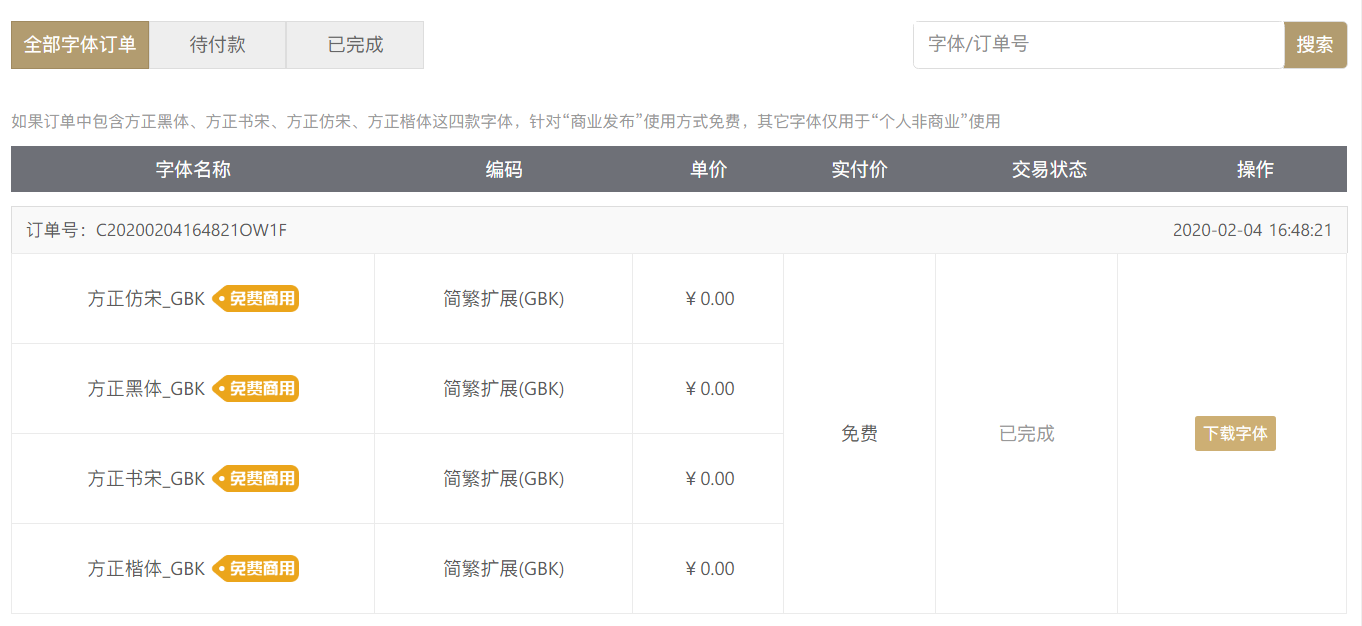
\includegraphics[width=0.9\textwidth]{founder.png}
\end{figure}

\subsection{其他中文字体}
如果你想完全自定义字体\footnote{这里仍然以方正字体为例。},你可以选择 \lstinline{chinesefont=nofont},然后在导言区设置
\begin{lstlisting}
\setCJKmainfont[BoldFont={FZHei-B01},ItalicFont={FZKai-Z03}]{FZShuSong-Z01}
\setCJKsansfont[BoldFont={FZHei-B01},ItalicFont={FZHei-B01}]{FZHei-B01}
\setCJKmonofont[BoldFont={FZHei-B01},ItalicFont={FZHei-B01}]{FZFangSong-Z02}
\setCJKfamilyfont{zhsong}{FZShuSong-Z01}
\setCJKfamilyfont{zhhei}{FZHei-B01}
\setCJKfamilyfont{zhkai}{FZKai-Z03}
\setCJKfamilyfont{zhfs}{FZFangSong-Z02}
\newcommand*{\songti}{\CJKfamily{zhsong}}
\newcommand*{\heiti}{\CJKfamily{zhhei}}
\newcommand*{\kaishu}{\CJKfamily{zhkai}}
\newcommand*{\fangsong}{\CJKfamily{zhfs}}
\end{lstlisting}

\chapter{ElegantBook 写作示例}

\begin{introduction}
  \item 积分定义~\ref{def:int}
  \item Fubini 定理~\ref{thm:fubi}
  \item 最优性原理~\ref{pro:max}
  \item 柯西列性质~\ref{property:cauchy}
  \item 韦达定理
\end{introduction}

\section{Lebesgue 积分}
在前面各章做了必要的准备后,本章开始介绍新的积分。在 Lebesgue 测度理论的基础上建立了 Lebesgue 积分,其被积函数和积分域更一般,可以对有界函数和无界函数统一处理。正是由于 Lebesgue 积分的这些特点,使得 Lebesgue 积分比 Riemann 积分具有在更一般条件下的极限定理和累次积分交换积分顺序的定理,这使得 Lebesgue 积分不仅在理论上更完善,而且在计算上更灵活有效。

Lebesgue 积分有几种不同的定义方式。我们将采用逐步定义非负简单函数,非负可测函数和一般可测函数积分的方式。

由于现代数学的许多分支如概率论、泛函分析、调和分析等常常用到一般空间上的测度与积分理论,在本章最后一节将介绍一般的测度空间上的积分。

\subsection{积分的定义}

我们将通过三个步骤定义可测函数的积分。首先定义非负简单函数的积分。以下设 $E$ 是 $\mathcal{R}^n$ 中的可测集。

\begin{definition}[可积性] \label{def:int} 
设 $ f(x)=\sum\limits_{i=1}^{k} a_i \chi_{A_i}(x)$ 是 $E$ 上的非负简单函数,其中 $\{A_1,A_2,\ldots,A_k\}$ 是 $E$ 上的一个可测分割,$a_1,a_2,\ldots,a_k$ 是非负实数。定义 $f$ 在 $E$ 上的积分为 $\int_{a}^b f(x)$
\begin{equation}
   \label{inter}
   \int_{E} f dx = \sum_{i=1}^k a_i m(A_i) \pi \alpha\beta\sigma\gamma\nu\xi\epsilon\varepsilon. \oint_{a}^b\ointop_{a}^b\prod_{i=1}^n
\end{equation}
一般情况下 $0 \leq \int_{E} f dx \leq \infty$。若 $\int_{E} f dx < \infty$,则称 $f$ 在 $E$ 上可积。
\end{definition}

一个自然的问题是,Lebesgue 积分与我们所熟悉的 Riemann 积分有什么联系和区别?在 4.4 在我们将详细讨论 Riemann 积分与 Lebesgue 积分的关系。这里只看一个简单的例子。设 $D(x)$ 是区间 $[0,1]$ 上的 Dirichlet 函数。即 $D(x)=\chi_{Q_0}(x)$,其中 $Q_0$ 表示 $[0,1]$ 中的有理数的全体。根据非负简单函数积分的定义,$D(x)$ 在 $[0,1]$ 上的 Lebesgue 积分为
\begin{equation}
   \label{inter2}
   \int_0^1 D(x)dx = \int_0^1 \chi_{Q_0} (x) dx = m(Q_0) = 0
\end{equation}
即 $D(x)$ 在 $[0,1]$ 上是 Lebesgue 可积的并且积分值为零。但 $D(x)$ 在 $[0,1]$ 上不是 Riemann 可积的。


有界变差函数是与单调函数有密切联系的一类函数。有界变差函数可以表示为两个单调递增函数之差。与单调函数一样,有界变差函数几乎处处可导。与单调函数不同,有界变差函数类对线性运算是封闭的,它们构成一线空间。练习题 \ref{exer:43} 是一个性质的证明。

\begin{exercise}\label{exer:43}
设 $f \notin\in L(\mathcal{R}^1)$,$g$ 是 $\mathcal{R}^1$ 上的有界可测函数。证明函数
\begin{equation}
   \label{ex:1}
   I(t) = \int_{\mathcal{R}^1} f(x+t)g(x)dx \quad t \in \mathcal{R}^1
\end{equation}
是 $\mathcal{R}^1$ 上的连续函数。 
\end{exercise}

\begin{solution}
即 $D(x)$ 在 $[0,1]$ 上是 Lebesgue 可积的并且积分值为零。但 $D(x)$ 在 $[0,1]$ 上不是 Riemann 可积的。
\end{solution}

\begin{proof}
即 $D(x)$ 在 $[0,1]$ 上是 Lebesgue 可积的并且积分值为零。但 $D(x)$ 在 $[0,1]$ 上不是 Riemann 可积的。
\end{proof}

\begin{theorem}[Fubini 定理] \label{thm:fubi} 
(1)若 $f(x,y)$ 是 $\mathcal{R}^p\times\mathcal{R}^q$ 上的非负可测函数,则对几乎处处的 $x\in \mathcal{R}^p$,$f(x,y)$ 作为 $y$ 的函数是 $\mathcal{R}^q$ 上的非负可测函数,$g(x)=\int_{\mathcal{R}^q}f(x,y) dy$ 是 $\mathcal{R}^p$ 上的非负可测函数。并且
\begin{equation}
   \label{eq:461}
   \int_{\mathcal{R}^p\times\mathcal{R}^q} f(x,y) dxdy=\int_{\mathcal{R}^p}\left(\int_{\mathcal{R}^q}f(x,y)dy\right)dx.
\end{equation}

(2)若 $f(x,y)$ 是 $\mathcal{R}^p\times\mathcal{R}^q$ 上的可积函数,则对几乎处处的 $x\in\mathcal{R}^p$,$f(x,y)$ 作为 $y$ 的函数是 $\mathcal{R}^q$ 上的可积函数,并且 $g(x)=\int_{\mathcal{R}^q}f(x,y) dy$ 是 $\mathcal{R}^p$ 上的可积函数。而且~\ref{eq:461} 成立。
\end{theorem}

\ref{thm:fubi}

\begin{note}
在本模板中,引理(lemma),推论(corollary)的样式和定理~\ref{thm:fubi} 的样式一致,包括颜色,仅仅只有计数器的设置不一样。
\end{note}

我们说一个实变或者复变量的实值或者复值函数是在区间上平方可积的,如果其绝对值的平方在该区间上的积分是有限的。所有在勒贝格积分意义下平方可积的可测函数构成一个希尔伯特空间,也就是所谓的 $L^2$ 空间,几乎处处相等的函数归为同一等价类。形式上,$L^2$ 是平方可积函数的空间和几乎处处为 0 的函数空间的商空间。

\begin{proposition}[最优性原理] \label{pro:max}
如果 $u^*$ 在 $[s,T]$ 上为最优解,则 $u^*$ 在 $[s, T]$ 任意子区间都是最优解,假设区间为 $[t_0, t_1]$ 的最优解为 $u^*$ ,则 $u(t_0)=u^{*}(t_0)$,即初始条件必须还是在 $u^*$ 上。
\end{proposition}

我们知道最小二乘法可以用来处理一组数据,可以从一组测定的数据中寻求变量之间的依赖关系,这种函数关系称为经验公式。本课题将介绍最小二乘法的精确定义及如何寻求点与点之间近似成线性关系时的经验公式。假定实验测得变量之间的 $n$ 个数据,则在平面上,可以得到 $n$ 个点,这种图形称为 “散点图”,从图中可以粗略看出这些点大致散落在某直线近旁, 我们认为其近似为一线性函数,下面介绍求解步骤。

\begin{figure}[htbp]
  \centering
  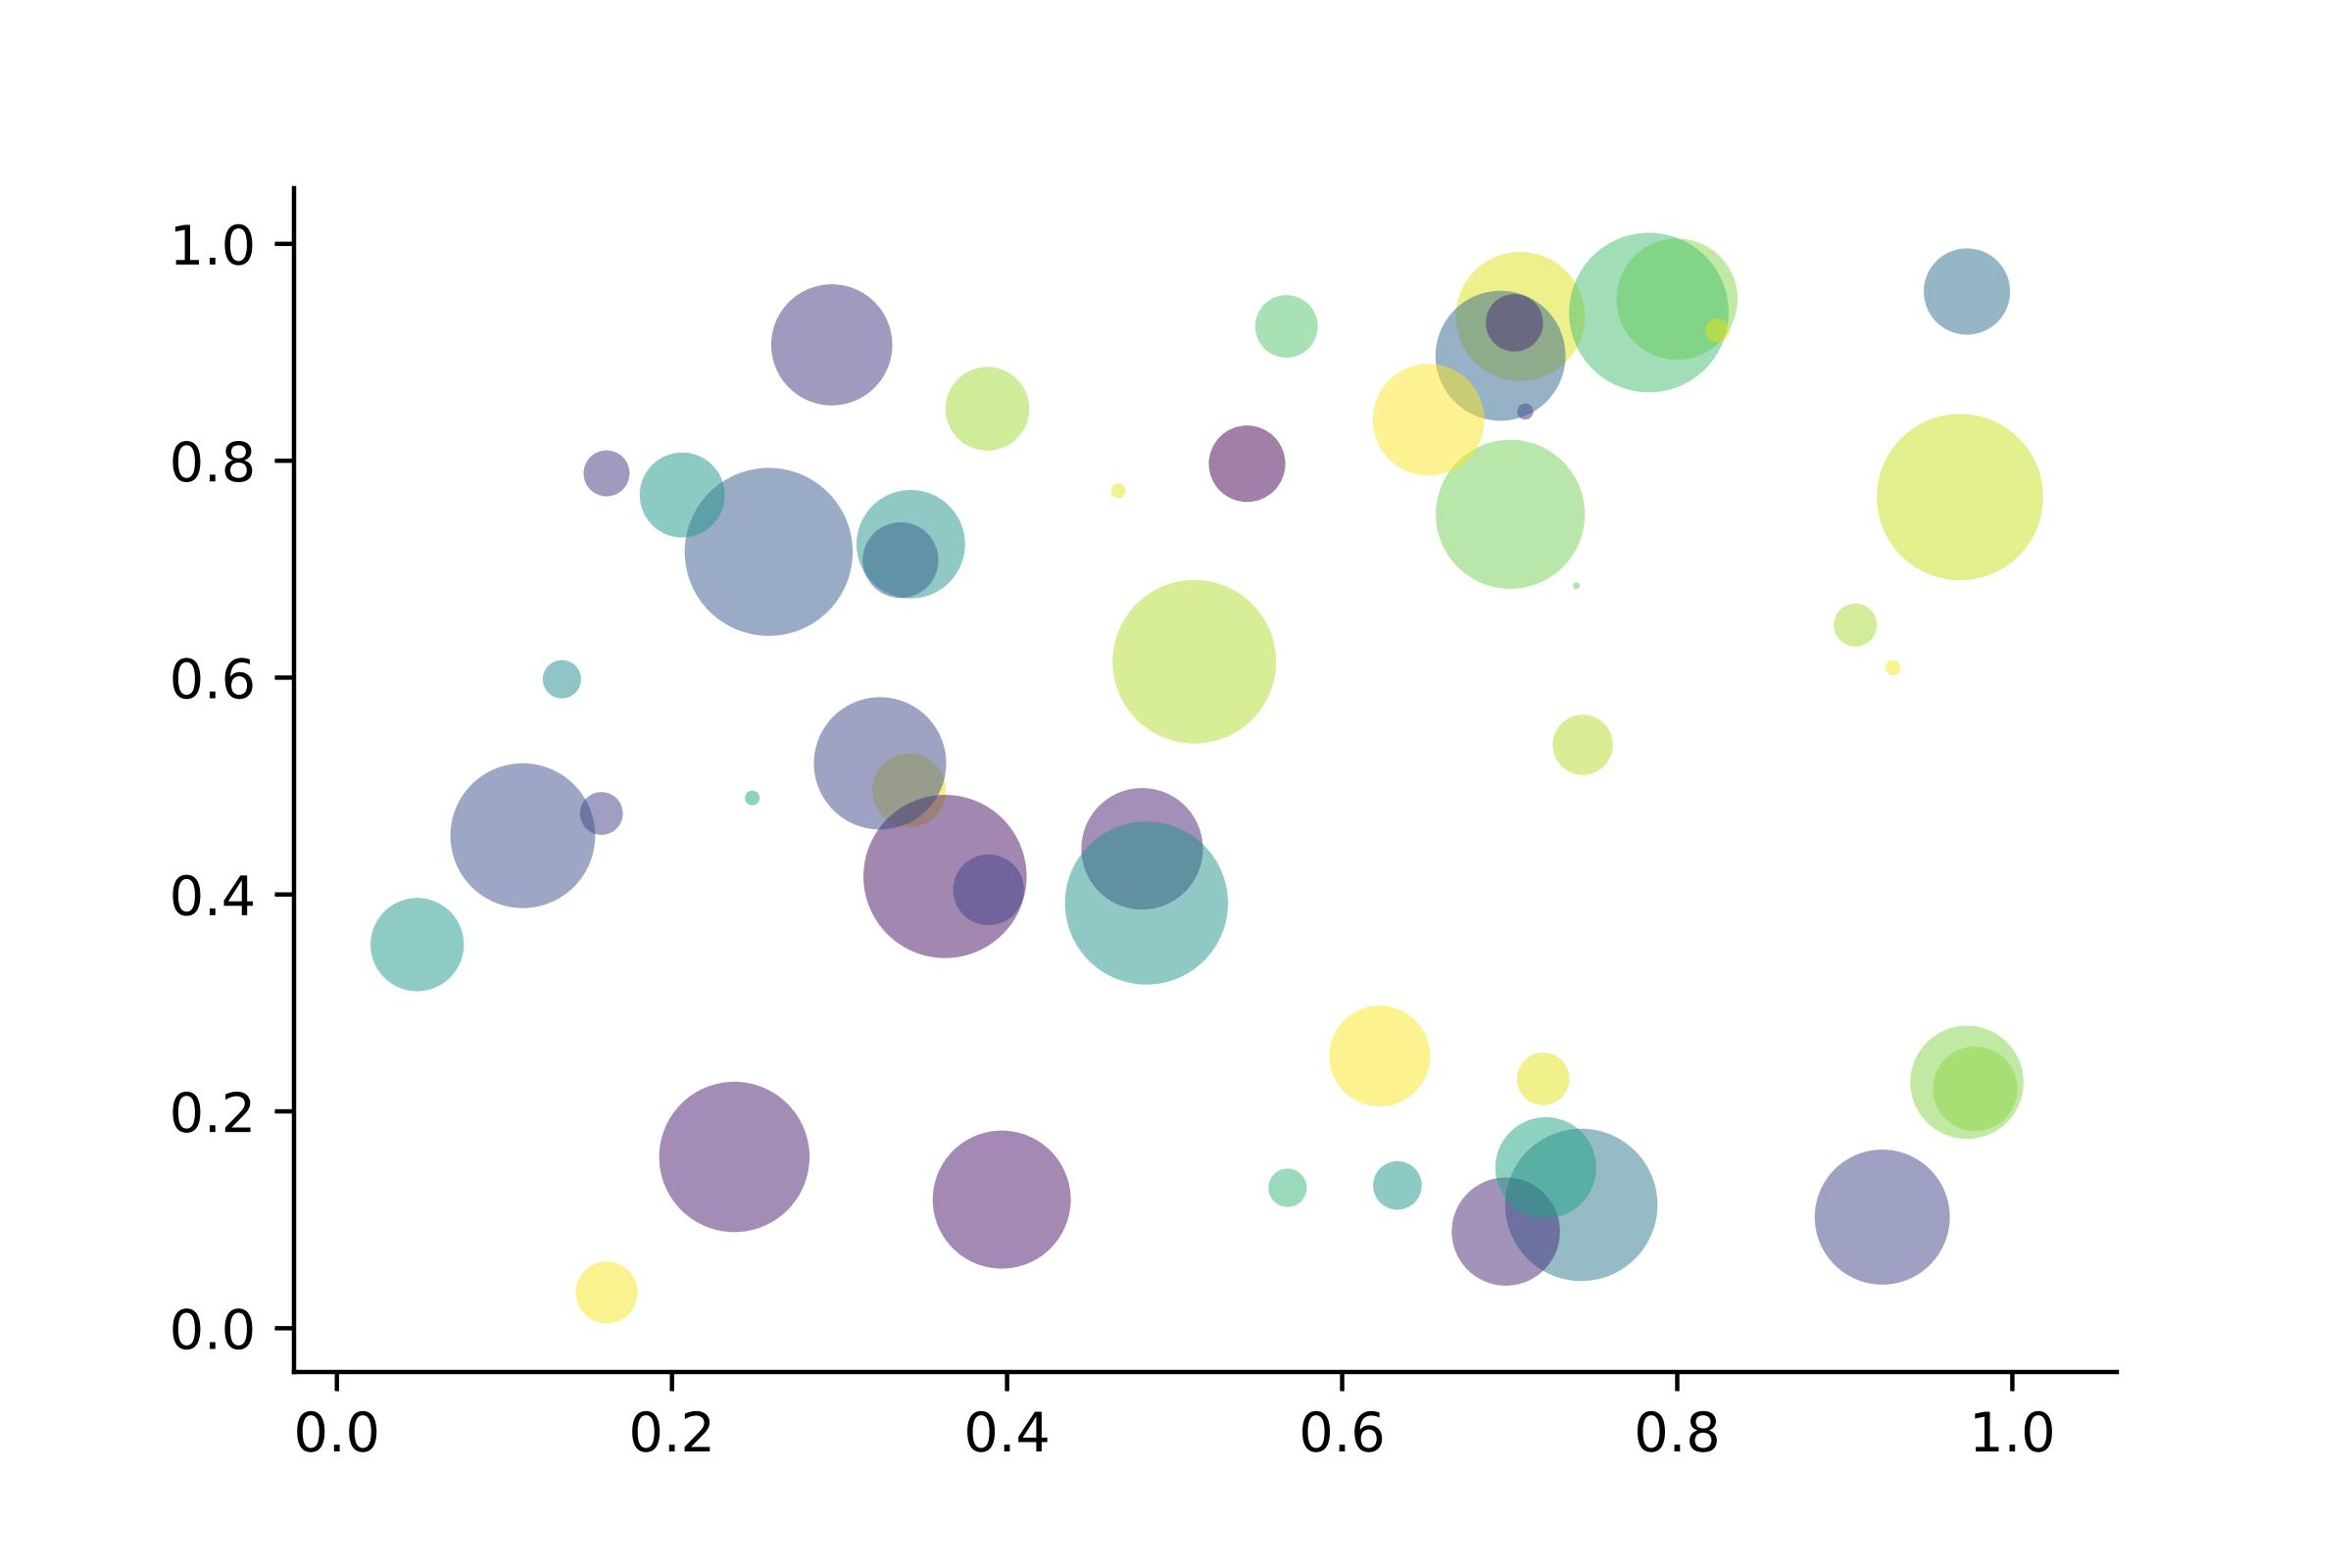
\includegraphics[width=0.6\textwidth]{scatter.jpg}
  \caption{散点图示例 $\hat{y}=a+bx$ \label{fig:scatter}}
\end{figure}

以最简单的一元线性模型来解释最小二乘法。什么是一元线性模型呢?监督学习中,如果预测的变量是离散的,我们称其为分类(如决策树,支持向量机等),如果预测的变量是连续的,我们称其为回归。回归分析中,如果只包括一个自变量和一个因变量,且二者的关系可用一条直线近似表示,这种回归分析称为一元线性回归分析。如果回归分析中包括两个或两个以上的自变量,且因变量和自变量之间是线性关系,则称为多元线性回归分析。对于二维空间线性是一条直线;对于三维空间线性是一个平面,对于多维空间线性是一个超平面。

\begin{property}\label{property:cauchy}
柯西列的性质
\begin{enumerate}
\item $\{x_k\}$ 是柯西列,则其子列 $\{x_k^i\}$ 也是柯西列。
\item $x_k\in \mathcal{R}^n$,$\rho(x,y)$ 是欧几里得空间,则柯西列收敛,$(\mathcal{R}^n,\rho)$ 空间是完备的。
\end{enumerate}
\end{property}

\begin{conclusion}
回归分析(regression analysis) 是确定两种或两种以上变量间相互依赖的定量关系的一种统计分析方法。运用十分广泛,回归分析按照涉及的变量的多少,分为一元回归和多元回归分析;按照因变量的多少,可分为简单回归分析和多重回归分析;按照自变量和因变量之间的关系类型,可分为线性回归分析和非线性回归分析。
\end{conclusion}

\begin{problemset}
\item 设 $A$ 为数域 $K$ 上的 $n$ 级矩阵。证明:如果 $K^n$ 中任意非零列向量都是 $A$ 的特征向量,则 $A$ 一定是数量矩阵。
\item 证明:不为零矩阵的幂零矩阵不能对角化。
\item 设 $A = (a_{ij})$ 是数域 $K$ 上的一个 $n$ 级上三角矩阵,证明:如果 $a_{11} = a_{22} = \cdots = a_{nn}$,并且至少有一个 $a_{kl} \not = 0 (k < l)$,则 $A$ 一定不能对角化。
\end{problemset}

\chapter{常见问题集}

我们根据用户社区反馈整理了下面一些常见的问题,用户在遇到问题时,应当首先查阅本手册和本部分的常见的问题。

\begin{enumerate}[itemsep=1.5ex]
  \item \question{有没有办法章节用“第一章,第一节,(一)”这种?}
    见前文介绍,可以使用 \lstinline{scheme=chinese} 设置。
  \item \question{大佬,我想把正文字体改为亮色,背景色改为黑灰色。}
    页面颜色可以使用 \lstinline{\pagecolor} 命令设置,文本命令可以参考\href{https://tex.stackexchange.com/questions/278544/xcolor-what-is-the-equivalent-of-default-text-color}{这里}进行设置。
  \item \question{\lstinline[breaklines]{Package ctex Error: CTeX fontset `Mac' is unavailable.}}
    在 Mac 系统下,中文编译请使用 \hologo{XeLaTeX}。
  \item \question{\lstinline{! LaTeX Error: Unknown option `scheme=plain' for package `ctex'.}}
    你用的 C\TeX{} 套装吧?这个里面的 \lstinline{ctex} 宏包已经是已经是 10 年前的了,与本模板使用的 \lstinline{ctex} 宏集有很大区别。不建议 C\TeX{} 套装了,请卸载并安装 \TeX{} Live 2021。
  \item \question{我该使用什么版本?}
    请务必使用\href{https://github.com/ElegantLaTeX/ElegantBook/releases}{最新正式发行版},发行版间不定期可能会有更新(修复 bug 或者改进之类),如果你在使用过程中没有遇到问题,不需要每次更新\href{https://github.com/ElegantLaTeX/ElegantBook/archive/master.zip}{最新版},但是在发行版更新之后,请尽可能使用最新版(发行版)!最新发行版可以在 GitHub 或者 \TeX{} Live 2021 内获取。
  \item \question{我该使用什么编辑器?}
    你可以使用 \TeX{} Live 2021 自带的编辑器 \TeX{}works 或者使用 \TeX{}studio,\TeX works 的自动补全,你可以参考我们的总结 \href{https://github.com/EthanDeng/texworks-autocomplete}{\TeX works 自动补全}。推荐使用 \TeX{} Live 2021 + \TeX{}studio。我自己用 VS Code 和 Sublime Text,相关的配置说明,请参考 \href{https://github.com/EthanDeng/vscode-latex}{\LaTeX{} 编译环境配置:Visual Studio Code 配置简介} 和 \href{https://github.com/EthanDeng/sublime-text-latex}{Sublime Text 搭建 \LaTeX{} 编写环境}。
  \item \question{您好,我们想用您的 ElegantBook 模板写一本书。关于机器学习的教材,希望获得您的授权,谢谢您的宝贵时间。}
    模板的使用修改都是自由的,你们声明模板来源以及模板地址(GitHub 地址)即可,其他未尽事宜按照开源协议 LPPL-1.3c。做好之后,如果方便的话,可以给我们一个链接,我把你们的教材放在 Elegant\LaTeX{} 用户作品集里。
  \item \question{请问交叉引用是什么?}
    本群和本模板适合有一定 \LaTeX{} 基础的用户使用,新手请先学习 \LaTeX{} 的基础,理解各种概念,否则你将寸步难行。
  \item \question{定义等环境中无法使用加粗命令么?}
    是这样的,默认中文并没加粗命令,如果你想在定义等环境中使用加粗命令,请使用 \lstinline{\heiti} 等字体命令,而不要使用 \lstinline{\textbf}。或者,你可以将 \lstinline|\textbf| 重新定义为 \lstinline|\heiti|。英文模式不存在这个问题。
  \item \question{代码高亮环境能用其他语言吗?}
    可以的,ElegantBook 模板用的是 \lstinline{listings} 宏包,你可以在环境(\lstinline{lstlisting})之后加上语言(比如 Python 使用 \lstinline{language=Python} 选项),全局语言修改请使用 \lstinline{lsset} 命令,更多信息请参考宏包文档。
  \item \question{群主,什么时候出 Beamer 的模板(主题),ElegantSlide 或者 ElegantBeamer?}
    由于 Beamer 中有一个很优秀的主题 \href{https://github.com/matze/mtheme}{Metropolis}。后续确定不会再出任何主题/模板,请大家根据需要修改已有主题。
\end{enumerate}

\chapter{版本更新历史}

根据用户的反馈,我们不断修正和完善模板。截止到此次更新,ElegantBook 模板在 GitHub 上有将近 100 次提交,正式发行版本(release)有 17 次。由于 3.00 之前版本与现在版本差异非常大,在此不列出 3.00 之前的更新内容。


\datechange{2021/05/02}{版本 4.1 正式发布。}

\begin{change}
  \item \textbf{重要改动}:由原先的 \hologo{BibTeX} 改为 biblatex 编译方式(后端为 \lstinline{biber}),请注意两者之间的差异;
  \item \textbf{重要改进}:修改对于定理写法兼容方式,提高数学公式代码的兼容性;
  \item 页面设置改动,默认页面更宽;方便书写和阅读;
  \item 支持目录文字以及页码跳转;
  \item 不再维护 \hologo{pdfLaTeX} 中文支持方式,请务必使用 \hologo{XeLaTeX} 编译中文文稿。
  \item 增加多个语言选项,法语 \lstinline{lang=fr}、荷兰语 \lstinline{lang=nl}、匈牙利语 \lstinline{lang=hu}、西班牙语 \lstinline{lang=es}、蒙古语 \lstinline{lang=mn} 等。
\end{change}


\datechange{2020/04/12}{版本 3.11 正式发布,\textcolor{red}{此版本为 3.x 最后版本。}}

\begin{change}
  \item \textbf{重要修正}:修复因为 \lstinline{gbt7714} 宏包更新导致的 \lstinline{natbib option clash} 错误;
  \item 由于 \lstinline{pgfornament} 宏包未被 \TeX{} Live 2020 收录,因此删除 base 相关的内容;
  \item 修复部分环境的空格问题;
  \item 增加了意大利语言选项 \lstinline{lang=it}。
\end{change}


\datechange{2020/02/10}{版本 3.10 正式发布}

\begin{change}
  \item 增加数学字体选项 \lstinline{math},可选项为 \lstinline{newtx} 和 \lstinline{cm}。\\
  \textbf{重要提示}:原先通过 \lstinline{newtxmath} 宏包设置的数学字体改为 \LaTeX{} 默认数学字体,如果需要保持原来的字体,需要显式声明数学字体(\lstinline{math=newtx});
  \item 新增中文字体选项 \lstinline{chinesefont},可选项为 \lstinline{ctexfont}、\lstinline{founder} 和 \lstinline{nofont}。
  \item 将封面作者信息设置为可选,并且增加自定义信息命令 \lstinline{\bioinfo};
  \item 在说明文档中增加版本历史,新增 \lstinline{\datechange} 命令和 \lstinline{change} 环境;
  \item 增加汉化章节选项 \lstinline{scheme},可选项为汉化 \lstinline{chinese};
  \item 由于 \lstinline{\lvert} 问题已经修复,重新调整 \lstinline{ctex} 宏包和 \lstinline{amsmath} 宏包位置。
  \item 修改页眉设置,去除了 \lstinline{\lastpage} 以避免 page anchor 问题,加入 \lstinline{\frontmatter}。
  \item 修改参考文献选项 \lstinline{cite},可选项为数字 \lstinline{numbers}、 作者-年份 \lstinline{authoryear} 以及上标 \lstinline{super}。
  \item 新增参考文献样式选项 \lstinline{bibstyle},并将英文模式下参考文献样式 \lstinline{apalike} 设置为默认值,中文仍然使用 \lstinline{gbt7714} 宏包设置。
\end{change}

\datechange{2019/08/18}{版本 3.09 正式发布}

\begin{change}
  \item \lstinline{\elegantpar} 存在 bug,删除 \lstinline{\elegantpar} 命令,建议用户改用 \lstinline{\marginnote} 和 \lstinline{\marginpar} 旁注命令。
  \item 积分操作符统一更改为 \lstinline{esint} 宏包设置;
  \item 新增目录选项 \lstinline{toc},可选项为单栏 \lstinline{onecol} 和双栏 \lstinline{twocol};
  \item 手动增加参考文献选项 \lstinline{cite},可选项为上标形式 \lstinline{super};
  \item 修正章节习题(\lstinline{problemset})环境。
\end{change}

\datechange{2019/05/28}{版本 3.08 正式发布}

\begin{change}
  \item 修复 \lstinline{\part} 命令。
  \item 引入 Note 模板中的 \lstinline{pad} 选项 \lstinline{device=pad}。
  \item 数学字体加入 \lstinline{mtpro2} 可选项 \lstinline{math=mtpro2},使用免费的 \lstinline{lite} 子集。
  \item 将参考文献默认显示方式 \lstinline{authoyear} 改为 \lstinline{numbers}。
  \item 引入旁注命令 \lstinline{\marginpar}(测试)。
  \item 新增章节摘要环境 \lstinline{introduction}。
  \item 新增章节习题环境 \lstinline{problemset}。
  \item 将 \lstinline{\equote} 重命名为 \lstinline{\extrainfo}。
  \item 完善说明文档,增加致谢部分。
\end{change}

\datechange{2019/04/15}{版本 3.07 正式发布}

\begin{change}
  \item 删除中英文自定义字体总设置。
  \item 新增颜色主题,并将原绿色默认主题设置为蓝色 \lstinline{color=blue}。
  \item 引入隐藏装饰图案选项 \lstinline{base},可选项有显示 \lstinline{show} 和隐藏 \lstinline{hide}。
  \item 新增定理模式 \lstinline{mode},可选项有简单模式 \lstinline{simple} 和炫彩模式 \lstinline{fancy}。
  \item 新增隐藏证明、答案等环境的选项 \lstinline{result=noanswer}。
\end{change}

\datechange{2019/02/25}{版本 3.06 正式发布}

\begin{change}
  \item 删除水印。
  \item 新封面,新装饰图案。
  \item 添加引言使用说明。
  \item 修复双面 \lstinline{twoside}。
  \item 美化列表环境。
  \item 增加 \lstinline{\subsubsection} 的设置。
  \item 将模板拆分成中英文语言模式。
  \item 使用 \lstinline{lstlisting} 添加代码高亮。
  \item 增加定理类环境使用说明。
\end{change}

\datechange{2019/01/22}{版本 3.05 正式发布}

\begin{change}
  \item 添加 \lstinline{xeCJK} 宏包中文支持方案。
  \item 修复模板之前对 Ti\textit{k}Z 单位的改动。
  \item 更新 logo 图。
\end{change}

\datechange{2019/01/15}{版本 3.04 正式发布}

\begin{change}
  \item 格式化模板代码。
  \item 增加 \lstinline{\equote} 命令。
  \item 修改 \lstinline{\date}。
\end{change}

\datechange{2019/01/08}{版本 3.03 正式发布}

\begin{change}
  \item 修复附录章节显示问题。
  \item 小幅优化封面代码。
\end{change}

\datechange{2018/12/31}{版本 3.02 正式发布}

\begin{change}
  \item 修复名字系列命令自定义格式时出现的空格问题,比如 \lstinline{\listfigurename}。
  \item 英文定理类名字改为中文名。
  \item 英文结构名改为中文。
\end{change}

\datechange{2018/12/16}{版本 3.01 正式发布}

\begin{change}
  \item 调整 \lstinline{ctex} 宏包。
  \item 说明文档增加更新内容。
\end{change}

\datechange{2018/12/06}{版本 3.00 正式发布}

\begin{change}
  \item 删除 \lstinline{mathpazo} 数学字体选项。
  \item 添加邮箱命令 \lstinline{\mailto}。
  \item 修改英文字体为 \lstinline{newtx} 系列,另外大型操作符号维持 cm 字体。
  \item 中文字体改用 \lstinline{ctex} 宏包自动设置。
  \item 删除 \lstinline{xeCJK} 字体设置,原因是不同系统字体不方便统一。
  \item 定理换用 \lstinline{tcolobox} 宏包定义,并基本维持原有的定理样式,优化显示效果,支持跨页;定理类名字重命名,如 etheorem 改为 theorem 等等。
  \item 删去自定义的缩进命令 \lstinline{\Eindent}。
  \item 添加参考文献宏包 \lstinline{natbib}。
  \item 颜色名字重命名。
\end{change}

\nocite{*} 
\printbibliography
\appendix

\chapter{基本数学工具}


本附录包括了计量经济学中用到的一些基本数学,我们扼要论述了求和算子的各种性质,研究了线性和某些非线性方程的性质,并复习了比例和百分数。我们还介绍了一些在应用计量经济学中常见的特殊函数,包括二次函数和自然对数,前 4 节只要求基本的代数技巧,第 5 节则对微分学进行了简要回顾;虽然要理解本书的大部分内容,微积分并非必需,但在一些章末附录和第 3 篇某些高深专题中,我们还是用到了微积分。

\section{求和算子与描述统计量}

\textbf{求和算子} 是用以表达多个数求和运算的一个缩略符号,它在统计学和计量经济学分析中扮演着重要作用。如果 $\{x_i: i=1, 2, \ldots, n\}$ 表示 $n$ 个数的一个序列,那么我们就把这 $n$ 个数的和写为:

\begin{equation}
\sum_{i=1}^n x_i \equiv x_1 + x_2 +\cdots + x_n
\end{equation}



\end{document}
